\documentclass[twoside]{book}

% Packages required by doxygen
\usepackage{fixltx2e}
\usepackage{calc}
\usepackage{doxygen}
\usepackage[export]{adjustbox} % also loads graphicx
\usepackage{graphicx}
\usepackage[utf8]{inputenc}
\usepackage{makeidx}
\usepackage{multicol}
\usepackage{multirow}
\PassOptionsToPackage{warn}{textcomp}
\usepackage{textcomp}
\usepackage[nointegrals]{wasysym}
\usepackage[table]{xcolor}

% Font selection
\usepackage[T1]{fontenc}
\usepackage[scaled=.90]{helvet}
\usepackage{courier}
\usepackage{amssymb}
\usepackage{sectsty}
\renewcommand{\familydefault}{\sfdefault}
\allsectionsfont{%
  \fontseries{bc}\selectfont%
  \color{darkgray}%
}
\renewcommand{\DoxyLabelFont}{%
  \fontseries{bc}\selectfont%
  \color{darkgray}%
}
\newcommand{\+}{\discretionary{\mbox{\scriptsize$\hookleftarrow$}}{}{}}

% Page & text layout
\usepackage{geometry}
\geometry{%
  a4paper,%
  top=2.5cm,%
  bottom=2.5cm,%
  left=2.5cm,%
  right=2.5cm%
}
\tolerance=750
\hfuzz=15pt
\hbadness=750
\setlength{\emergencystretch}{15pt}
\setlength{\parindent}{0cm}
\setlength{\parskip}{3ex plus 2ex minus 2ex}
\makeatletter
\renewcommand{\paragraph}{%
  \@startsection{paragraph}{4}{0ex}{-1.0ex}{1.0ex}{%
    \normalfont\normalsize\bfseries\SS@parafont%
  }%
}
\renewcommand{\subparagraph}{%
  \@startsection{subparagraph}{5}{0ex}{-1.0ex}{1.0ex}{%
    \normalfont\normalsize\bfseries\SS@subparafont%
  }%
}
\makeatother

% Headers & footers
\usepackage{fancyhdr}
\pagestyle{fancyplain}
\fancyhead[LE]{\fancyplain{}{\bfseries\thepage}}
\fancyhead[CE]{\fancyplain{}{}}
\fancyhead[RE]{\fancyplain{}{\bfseries\leftmark}}
\fancyhead[LO]{\fancyplain{}{\bfseries\rightmark}}
\fancyhead[CO]{\fancyplain{}{}}
\fancyhead[RO]{\fancyplain{}{\bfseries\thepage}}
\fancyfoot[LE]{\fancyplain{}{}}
\fancyfoot[CE]{\fancyplain{}{}}
\fancyfoot[RE]{\fancyplain{}{\bfseries\scriptsize Generated by Doxygen }}
\fancyfoot[LO]{\fancyplain{}{\bfseries\scriptsize Generated by Doxygen }}
\fancyfoot[CO]{\fancyplain{}{}}
\fancyfoot[RO]{\fancyplain{}{}}
\renewcommand{\footrulewidth}{0.4pt}
\renewcommand{\chaptermark}[1]{%
  \markboth{#1}{}%
}
\renewcommand{\sectionmark}[1]{%
  \markright{\thesection\ #1}%
}

% Indices & bibliography
\usepackage{natbib}
\usepackage[titles]{tocloft}
\setcounter{tocdepth}{3}
\setcounter{secnumdepth}{5}
\makeindex

% Hyperlinks (required, but should be loaded last)
\usepackage{ifpdf}
\ifpdf
  \usepackage[pdftex,pagebackref=true]{hyperref}
\else
  \usepackage[ps2pdf,pagebackref=true]{hyperref}
\fi
\hypersetup{%
  colorlinks=true,%
  linkcolor=blue,%
  citecolor=blue,%
  unicode%
}

% Custom commands
\newcommand{\clearemptydoublepage}{%
  \newpage{\pagestyle{empty}\cleardoublepage}%
}

\usepackage{caption}
\captionsetup{labelsep=space,justification=centering,font={bf},singlelinecheck=off,skip=4pt,position=top}

%===== C O N T E N T S =====

\begin{document}

% Titlepage & ToC
\hypersetup{pageanchor=false,
             bookmarksnumbered=true,
             pdfencoding=unicode
            }
\pagenumbering{alph}
\begin{titlepage}
\vspace*{7cm}
\begin{center}%
{\Large Space Invaders \\[1ex]\large 1.\+0.\+0 }\\
\vspace*{1cm}
{\large Generated by Doxygen 1.8.14}\\
\end{center}
\end{titlepage}
\clearemptydoublepage
\pagenumbering{roman}
\tableofcontents
\clearemptydoublepage
\pagenumbering{arabic}
\hypersetup{pageanchor=true}

%--- Begin generated contents ---
\chapter{Hierarchical Index}
\section{Class Hierarchy}
This inheritance list is sorted roughly, but not completely, alphabetically\+:\begin{DoxyCompactList}
\item \contentsline{section}{Barricade}{\pageref{class_barricade}}{}
\item \contentsline{section}{Collision\+Manager}{\pageref{class_collision_manager}}{}
\item \contentsline{section}{Game\+Handler}{\pageref{class_game_handler}}{}
\item \contentsline{section}{Game\+Object}{\pageref{class_game_object}}{}
\begin{DoxyCompactList}
\item \contentsline{section}{Barricade\+Block}{\pageref{class_barricade_block}}{}
\item \contentsline{section}{Enemy}{\pageref{class_enemy}}{}
\item \contentsline{section}{Mystery\+Ship}{\pageref{class_mystery_ship}}{}
\item \contentsline{section}{Player}{\pageref{class_player}}{}
\item \contentsline{section}{Projectile}{\pageref{class_projectile}}{}
\begin{DoxyCompactList}
\item \contentsline{section}{Enemy\+Attack}{\pageref{class_enemy_attack}}{}
\item \contentsline{section}{Laser}{\pageref{class_laser}}{}
\item \contentsline{section}{Snake}{\pageref{class_snake}}{}
\end{DoxyCompactList}
\end{DoxyCompactList}
\item \contentsline{section}{Game\+Objects\+Manager}{\pageref{class_game_objects_manager}}{}
\item \contentsline{section}{Input\+Manager}{\pageref{class_input_manager}}{}
\item \contentsline{section}{Objects\+Pool}{\pageref{class_objects_pool}}{}
\item \contentsline{section}{Sound\+Manager}{\pageref{class_sound_manager}}{}
\item \contentsline{section}{Text}{\pageref{class_text}}{}
\item \contentsline{section}{Text\+Renderer}{\pageref{class_text_renderer}}{}
\item \contentsline{section}{Texture\+Manager}{\pageref{class_texture_manager}}{}
\item \contentsline{section}{Game\+Object\+:\+:Vector2D}{\pageref{struct_game_object_1_1_vector2_d}}{}
\end{DoxyCompactList}

\chapter{Class Index}
\section{Class List}
Here are the classes, structs, unions and interfaces with brief descriptions\+:\begin{DoxyCompactList}
\item\contentsline{section}{\mbox{\hyperlink{class_barricade}{Barricade}} }{\pageref{class_barricade}}{}
\item\contentsline{section}{\mbox{\hyperlink{class_barricade_block}{Barricade\+Block}} }{\pageref{class_barricade_block}}{}
\item\contentsline{section}{\mbox{\hyperlink{class_collision_manager}{Collision\+Manager}} }{\pageref{class_collision_manager}}{}
\item\contentsline{section}{\mbox{\hyperlink{class_enemy}{Enemy}} }{\pageref{class_enemy}}{}
\item\contentsline{section}{\mbox{\hyperlink{class_enemy_attack}{Enemy\+Attack}} }{\pageref{class_enemy_attack}}{}
\item\contentsline{section}{\mbox{\hyperlink{class_game_handler}{Game\+Handler}} }{\pageref{class_game_handler}}{}
\item\contentsline{section}{\mbox{\hyperlink{class_game_object}{Game\+Object}} }{\pageref{class_game_object}}{}
\item\contentsline{section}{\mbox{\hyperlink{class_game_objects_manager}{Game\+Objects\+Manager}} }{\pageref{class_game_objects_manager}}{}
\item\contentsline{section}{\mbox{\hyperlink{class_input_manager}{Input\+Manager}} }{\pageref{class_input_manager}}{}
\item\contentsline{section}{\mbox{\hyperlink{class_laser}{Laser}} }{\pageref{class_laser}}{}
\item\contentsline{section}{\mbox{\hyperlink{class_mystery_ship}{Mystery\+Ship}} }{\pageref{class_mystery_ship}}{}
\item\contentsline{section}{\mbox{\hyperlink{class_objects_pool}{Objects\+Pool}} }{\pageref{class_objects_pool}}{}
\item\contentsline{section}{\mbox{\hyperlink{class_player}{Player}} }{\pageref{class_player}}{}
\item\contentsline{section}{\mbox{\hyperlink{class_projectile}{Projectile}} }{\pageref{class_projectile}}{}
\item\contentsline{section}{\mbox{\hyperlink{class_snake}{Snake}} }{\pageref{class_snake}}{}
\item\contentsline{section}{\mbox{\hyperlink{class_sound_manager}{Sound\+Manager}} }{\pageref{class_sound_manager}}{}
\item\contentsline{section}{\mbox{\hyperlink{class_text}{Text}} }{\pageref{class_text}}{}
\item\contentsline{section}{\mbox{\hyperlink{class_text_renderer}{Text\+Renderer}} }{\pageref{class_text_renderer}}{}
\item\contentsline{section}{\mbox{\hyperlink{class_texture_manager}{Texture\+Manager}} }{\pageref{class_texture_manager}}{}
\item\contentsline{section}{\mbox{\hyperlink{struct_game_object_1_1_vector2_d}{Game\+Object\+::\+Vector2D}} }{\pageref{struct_game_object_1_1_vector2_d}}{}
\end{DoxyCompactList}

\chapter{File Index}
\section{File List}
Here is a list of all files with brief descriptions\+:\begin{DoxyCompactList}
\item\contentsline{section}{Eksamen\+Base/\mbox{\hyperlink{_eksamen_base_8cpp}{Eksamen\+Base.\+cpp}} }{\pageref{_eksamen_base_8cpp}}{}
\item\contentsline{section}{Eksamen\+Base/\+Game\+Objects/\mbox{\hyperlink{_enemy_8cpp}{Enemy.\+cpp}} }{\pageref{_enemy_8cpp}}{}
\item\contentsline{section}{Eksamen\+Base/\+Game\+Objects/\mbox{\hyperlink{_enemy_8h}{Enemy.\+h}} }{\pageref{_enemy_8h}}{}
\item\contentsline{section}{Eksamen\+Base/\+Game\+Objects/\mbox{\hyperlink{_enemy_attack_8cpp}{Enemy\+Attack.\+cpp}} }{\pageref{_enemy_attack_8cpp}}{}
\item\contentsline{section}{Eksamen\+Base/\+Game\+Objects/\mbox{\hyperlink{_enemy_attack_8h}{Enemy\+Attack.\+h}} }{\pageref{_enemy_attack_8h}}{}
\item\contentsline{section}{Eksamen\+Base/\+Game\+Objects/\mbox{\hyperlink{_game_object_8cpp}{Game\+Object.\+cpp}} }{\pageref{_game_object_8cpp}}{}
\item\contentsline{section}{Eksamen\+Base/\+Game\+Objects/\mbox{\hyperlink{_game_object_8h}{Game\+Object.\+h}} }{\pageref{_game_object_8h}}{}
\item\contentsline{section}{Eksamen\+Base/\+Game\+Objects/\mbox{\hyperlink{_laser_8cpp}{Laser.\+cpp}} }{\pageref{_laser_8cpp}}{}
\item\contentsline{section}{Eksamen\+Base/\+Game\+Objects/\mbox{\hyperlink{_laser_8h}{Laser.\+h}} }{\pageref{_laser_8h}}{}
\item\contentsline{section}{Eksamen\+Base/\+Game\+Objects/\mbox{\hyperlink{_player_8cpp}{Player.\+cpp}} }{\pageref{_player_8cpp}}{}
\item\contentsline{section}{Eksamen\+Base/\+Game\+Objects/\mbox{\hyperlink{_player_8h}{Player.\+h}} }{\pageref{_player_8h}}{}
\item\contentsline{section}{Eksamen\+Base/\+Game\+Objects/\mbox{\hyperlink{_projectile_8cpp}{Projectile.\+cpp}} }{\pageref{_projectile_8cpp}}{}
\item\contentsline{section}{Eksamen\+Base/\+Game\+Objects/\mbox{\hyperlink{_projectile_8h}{Projectile.\+h}} }{\pageref{_projectile_8h}}{}
\item\contentsline{section}{Eksamen\+Base/\+Game\+Objects/\mbox{\hyperlink{_snake_8cpp}{Snake.\+cpp}} }{\pageref{_snake_8cpp}}{}
\item\contentsline{section}{Eksamen\+Base/\+Game\+Objects/\mbox{\hyperlink{_snake_8h}{Snake.\+h}} }{\pageref{_snake_8h}}{}
\item\contentsline{section}{Eksamen\+Base/\+Handlers/\mbox{\hyperlink{_collision_manager_8cpp}{Collision\+Manager.\+cpp}} }{\pageref{_collision_manager_8cpp}}{}
\item\contentsline{section}{Eksamen\+Base/\+Handlers/\mbox{\hyperlink{_collision_manager_8h}{Collision\+Manager.\+h}} }{\pageref{_collision_manager_8h}}{}
\item\contentsline{section}{Eksamen\+Base/\+Handlers/\mbox{\hyperlink{_game_handler_8cpp}{Game\+Handler.\+cpp}} }{\pageref{_game_handler_8cpp}}{}
\item\contentsline{section}{Eksamen\+Base/\+Handlers/\mbox{\hyperlink{_game_handler_8h}{Game\+Handler.\+h}} }{\pageref{_game_handler_8h}}{}
\item\contentsline{section}{Eksamen\+Base/\+Handlers/\mbox{\hyperlink{_game_objects_manager_8cpp}{Game\+Objects\+Manager.\+cpp}} }{\pageref{_game_objects_manager_8cpp}}{}
\item\contentsline{section}{Eksamen\+Base/\+Handlers/\mbox{\hyperlink{_game_objects_manager_8h}{Game\+Objects\+Manager.\+h}} }{\pageref{_game_objects_manager_8h}}{}
\item\contentsline{section}{Eksamen\+Base/\+Handlers/\mbox{\hyperlink{_input_manager_8cpp}{Input\+Manager.\+cpp}} }{\pageref{_input_manager_8cpp}}{}
\item\contentsline{section}{Eksamen\+Base/\+Handlers/\mbox{\hyperlink{_input_manager_8h}{Input\+Manager.\+h}} }{\pageref{_input_manager_8h}}{}
\item\contentsline{section}{Eksamen\+Base/\+Handlers/\mbox{\hyperlink{_sound_manager_8cpp}{Sound\+Manager.\+cpp}} }{\pageref{_sound_manager_8cpp}}{}
\item\contentsline{section}{Eksamen\+Base/\+Handlers/\mbox{\hyperlink{_sound_manager_8h}{Sound\+Manager.\+h}} }{\pageref{_sound_manager_8h}}{}
\item\contentsline{section}{Eksamen\+Base/\+Handlers/\mbox{\hyperlink{_text_8cpp}{Text.\+cpp}} }{\pageref{_text_8cpp}}{}
\item\contentsline{section}{Eksamen\+Base/\+Handlers/\mbox{\hyperlink{_text_8h}{Text.\+h}} }{\pageref{_text_8h}}{}
\item\contentsline{section}{Eksamen\+Base/\+Handlers/\mbox{\hyperlink{_text_renderer_8cpp}{Text\+Renderer.\+cpp}} }{\pageref{_text_renderer_8cpp}}{}
\item\contentsline{section}{Eksamen\+Base/\+Handlers/\mbox{\hyperlink{_text_renderer_8h}{Text\+Renderer.\+h}} }{\pageref{_text_renderer_8h}}{}
\item\contentsline{section}{Eksamen\+Base/\+Handlers/\mbox{\hyperlink{_texture_manager_8cpp}{Texture\+Manager.\+cpp}} }{\pageref{_texture_manager_8cpp}}{}
\item\contentsline{section}{Eksamen\+Base/\+Handlers/\mbox{\hyperlink{_texture_manager_8h}{Texture\+Manager.\+h}} }{\pageref{_texture_manager_8h}}{}
\end{DoxyCompactList}

\chapter{Class Documentation}
\hypertarget{class_barricade}{}\section{Barricade Class Reference}
\label{class_barricade}\index{Barricade@{Barricade}}


{\ttfamily \#include $<$Barricade.\+h$>$}

\subsection*{Public Member Functions}
\begin{DoxyCompactItemize}
\item 
\mbox{\hyperlink{class_barricade_a2dfad888aded7d69ae2649e545103110}{Barricade}} (S\+D\+L\+\_\+\+Renderer $\ast$renderer, int x, int y)
\item 
\mbox{\hyperlink{class_barricade_ac74ebf54383e25f526e721964d6e4863}{$\sim$\+Barricade}} ()
\item 
void \mbox{\hyperlink{class_barricade_afae6747d40e49e937efaa1dd063a4461}{Reset\+Barricade\+Blocks}} ()
\begin{DoxyCompactList}\small\item\em Resets the barricadeblocks \end{DoxyCompactList}\end{DoxyCompactItemize}


\subsection{Constructor \& Destructor Documentation}
\mbox{\Hypertarget{class_barricade_a2dfad888aded7d69ae2649e545103110}\label{class_barricade_a2dfad888aded7d69ae2649e545103110}} 
\index{Barricade@{Barricade}!Barricade@{Barricade}}
\index{Barricade@{Barricade}!Barricade@{Barricade}}
\subsubsection{\texorpdfstring{Barricade()}{Barricade()}}
{\footnotesize\ttfamily Barricade\+::\+Barricade (\begin{DoxyParamCaption}\item[{S\+D\+L\+\_\+\+Renderer $\ast$}]{renderer,  }\item[{int}]{x,  }\item[{int}]{y }\end{DoxyParamCaption})}

\mbox{\Hypertarget{class_barricade_ac74ebf54383e25f526e721964d6e4863}\label{class_barricade_ac74ebf54383e25f526e721964d6e4863}} 
\index{Barricade@{Barricade}!````~Barricade@{$\sim$\+Barricade}}
\index{````~Barricade@{$\sim$\+Barricade}!Barricade@{Barricade}}
\subsubsection{\texorpdfstring{$\sim$\+Barricade()}{~Barricade()}}
{\footnotesize\ttfamily Barricade\+::$\sim$\+Barricade (\begin{DoxyParamCaption}{ }\end{DoxyParamCaption})}



\subsection{Member Function Documentation}
\mbox{\Hypertarget{class_barricade_afae6747d40e49e937efaa1dd063a4461}\label{class_barricade_afae6747d40e49e937efaa1dd063a4461}} 
\index{Barricade@{Barricade}!Reset\+Barricade\+Blocks@{Reset\+Barricade\+Blocks}}
\index{Reset\+Barricade\+Blocks@{Reset\+Barricade\+Blocks}!Barricade@{Barricade}}
\subsubsection{\texorpdfstring{Reset\+Barricade\+Blocks()}{ResetBarricadeBlocks()}}
{\footnotesize\ttfamily void Barricade\+::\+Reset\+Barricade\+Blocks (\begin{DoxyParamCaption}{ }\end{DoxyParamCaption})}



Resets the barricadeblocks 



The documentation for this class was generated from the following files\+:\begin{DoxyCompactItemize}
\item 
Eksamen\+Base/\+Game\+Objects/\mbox{\hyperlink{_barricade_8h}{Barricade.\+h}}\item 
Eksamen\+Base/\+Game\+Objects/\mbox{\hyperlink{_barricade_8cpp}{Barricade.\+cpp}}\end{DoxyCompactItemize}

\hypertarget{class_barricade_block}{}\section{Barricade\+Block Class Reference}
\label{class_barricade_block}\index{Barricade\+Block@{Barricade\+Block}}


{\ttfamily \#include $<$Barricade\+Block.\+h$>$}

Inheritance diagram for Barricade\+Block\+:\begin{figure}[H]
\begin{center}
\leavevmode
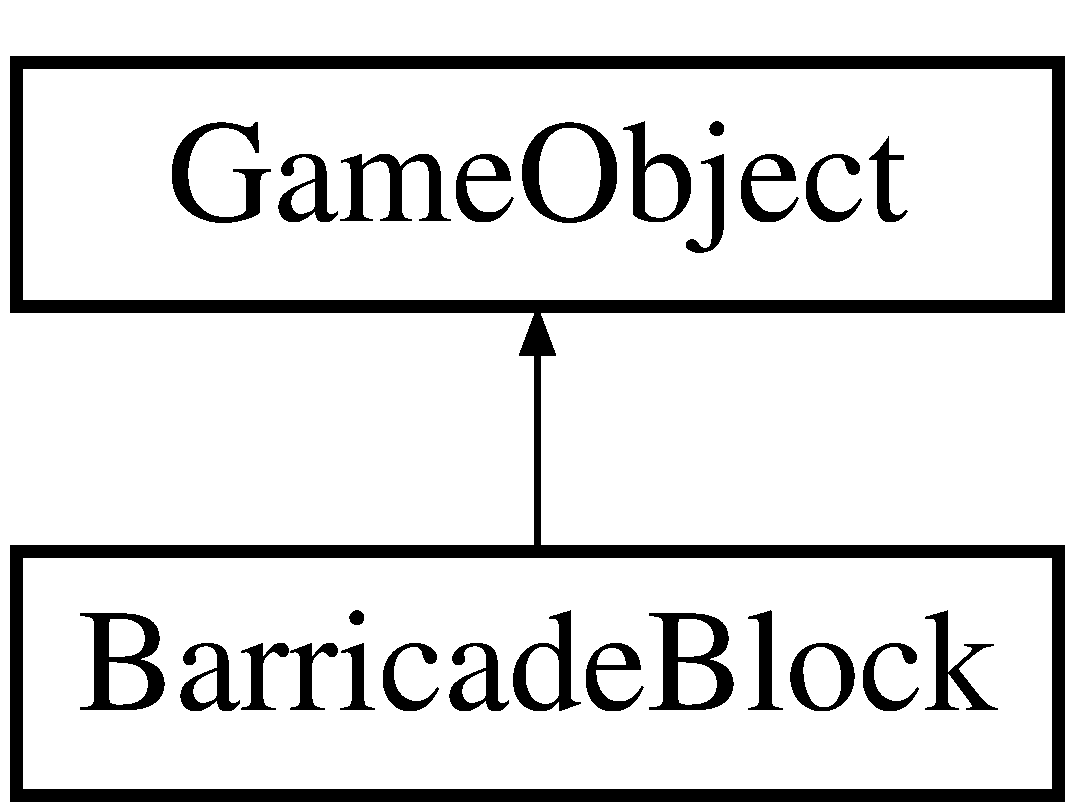
\includegraphics[height=2.000000cm]{class_barricade_block}
\end{center}
\end{figure}
\subsection*{Public Member Functions}
\begin{DoxyCompactItemize}
\item 
\mbox{\hyperlink{class_barricade_block_a497dcd5806e7a26f3c4d5e55e5a9be61}{Barricade\+Block}} (S\+D\+L\+\_\+\+Renderer $\ast$renderer, int x, int y)
\item 
\mbox{\hyperlink{class_barricade_block_ae4a2910fc259d532cb07179b8da76c4e}{$\sim$\+Barricade\+Block}} ()
\item 
void \mbox{\hyperlink{class_barricade_block_ac01d18a8afea6f0b15c7ec7b0167c7f1}{Logic}} ()
\item 
void \mbox{\hyperlink{class_barricade_block_adc4d1d90b1d7ad2a6b043aef0a9886d2}{Input}} ()
\end{DoxyCompactItemize}
\subsection*{Additional Inherited Members}


\subsection{Constructor \& Destructor Documentation}
\mbox{\Hypertarget{class_barricade_block_a497dcd5806e7a26f3c4d5e55e5a9be61}\label{class_barricade_block_a497dcd5806e7a26f3c4d5e55e5a9be61}} 
\index{Barricade\+Block@{Barricade\+Block}!Barricade\+Block@{Barricade\+Block}}
\index{Barricade\+Block@{Barricade\+Block}!Barricade\+Block@{Barricade\+Block}}
\subsubsection{\texorpdfstring{Barricade\+Block()}{BarricadeBlock()}}
{\footnotesize\ttfamily Barricade\+Block\+::\+Barricade\+Block (\begin{DoxyParamCaption}\item[{S\+D\+L\+\_\+\+Renderer $\ast$}]{renderer,  }\item[{int}]{x,  }\item[{int}]{y }\end{DoxyParamCaption})}

\mbox{\Hypertarget{class_barricade_block_ae4a2910fc259d532cb07179b8da76c4e}\label{class_barricade_block_ae4a2910fc259d532cb07179b8da76c4e}} 
\index{Barricade\+Block@{Barricade\+Block}!````~Barricade\+Block@{$\sim$\+Barricade\+Block}}
\index{````~Barricade\+Block@{$\sim$\+Barricade\+Block}!Barricade\+Block@{Barricade\+Block}}
\subsubsection{\texorpdfstring{$\sim$\+Barricade\+Block()}{~BarricadeBlock()}}
{\footnotesize\ttfamily Barricade\+Block\+::$\sim$\+Barricade\+Block (\begin{DoxyParamCaption}{ }\end{DoxyParamCaption})}



\subsection{Member Function Documentation}
\mbox{\Hypertarget{class_barricade_block_adc4d1d90b1d7ad2a6b043aef0a9886d2}\label{class_barricade_block_adc4d1d90b1d7ad2a6b043aef0a9886d2}} 
\index{Barricade\+Block@{Barricade\+Block}!Input@{Input}}
\index{Input@{Input}!Barricade\+Block@{Barricade\+Block}}
\subsubsection{\texorpdfstring{Input()}{Input()}}
{\footnotesize\ttfamily void Barricade\+Block\+::\+Input (\begin{DoxyParamCaption}{ }\end{DoxyParamCaption})\hspace{0.3cm}{\ttfamily [virtual]}}



Reimplemented from \mbox{\hyperlink{class_game_object_a430742cf91abb99337c556c88bef880a}{Game\+Object}}.

\mbox{\Hypertarget{class_barricade_block_ac01d18a8afea6f0b15c7ec7b0167c7f1}\label{class_barricade_block_ac01d18a8afea6f0b15c7ec7b0167c7f1}} 
\index{Barricade\+Block@{Barricade\+Block}!Logic@{Logic}}
\index{Logic@{Logic}!Barricade\+Block@{Barricade\+Block}}
\subsubsection{\texorpdfstring{Logic()}{Logic()}}
{\footnotesize\ttfamily void Barricade\+Block\+::\+Logic (\begin{DoxyParamCaption}{ }\end{DoxyParamCaption})\hspace{0.3cm}{\ttfamily [virtual]}}



Reimplemented from \mbox{\hyperlink{class_game_object_a79510ffc77339fe850491dce9f580fa9}{Game\+Object}}.



The documentation for this class was generated from the following files\+:\begin{DoxyCompactItemize}
\item 
Eksamen\+Base/\+Game\+Objects/\mbox{\hyperlink{_barricade_block_8h}{Barricade\+Block.\+h}}\item 
Eksamen\+Base/\+Game\+Objects/\mbox{\hyperlink{_barricade_block_8cpp}{Barricade\+Block.\+cpp}}\end{DoxyCompactItemize}

\hypertarget{class_collision_manager}{}\section{Collision\+Manager Class Reference}
\label{class_collision_manager}\index{Collision\+Manager@{Collision\+Manager}}


{\ttfamily \#include $<$Collision\+Manager.\+h$>$}

\subsection*{Public Member Functions}
\begin{DoxyCompactItemize}
\item 
\mbox{\hyperlink{class_collision_manager_acdbb3c842f0ef1c7a028d3f080855766}{$\sim$\+Collision\+Manager}} ()
\item 
std\+::vector$<$ \mbox{\hyperlink{class_game_object}{Game\+Object}} $\ast$ $>$ $\ast$ \mbox{\hyperlink{class_collision_manager_aa36e8b56d10fc36677a8a9bb76891c58}{On\+Collision}} (\mbox{\hyperlink{class_game_object}{Game\+Object}} $\ast$game\+Object)
\begin{DoxyCompactList}\small\item\em When there happens a collision with given object This method will return a vector with the objects being collided with. \end{DoxyCompactList}\end{DoxyCompactItemize}
\subsection*{Static Public Member Functions}
\begin{DoxyCompactItemize}
\item 
static \mbox{\hyperlink{class_collision_manager}{Collision\+Manager}} \& \mbox{\hyperlink{class_collision_manager_af7ae5c9cd14ffea044059e17225d3d1c}{get\+Instance}} ()
\end{DoxyCompactItemize}


\subsection{Constructor \& Destructor Documentation}
\mbox{\Hypertarget{class_collision_manager_acdbb3c842f0ef1c7a028d3f080855766}\label{class_collision_manager_acdbb3c842f0ef1c7a028d3f080855766}} 
\index{Collision\+Manager@{Collision\+Manager}!````~Collision\+Manager@{$\sim$\+Collision\+Manager}}
\index{````~Collision\+Manager@{$\sim$\+Collision\+Manager}!Collision\+Manager@{Collision\+Manager}}
\subsubsection{\texorpdfstring{$\sim$\+Collision\+Manager()}{~CollisionManager()}}
{\footnotesize\ttfamily Collision\+Manager\+::$\sim$\+Collision\+Manager (\begin{DoxyParamCaption}{ }\end{DoxyParamCaption})}



\subsection{Member Function Documentation}
\mbox{\Hypertarget{class_collision_manager_af7ae5c9cd14ffea044059e17225d3d1c}\label{class_collision_manager_af7ae5c9cd14ffea044059e17225d3d1c}} 
\index{Collision\+Manager@{Collision\+Manager}!get\+Instance@{get\+Instance}}
\index{get\+Instance@{get\+Instance}!Collision\+Manager@{Collision\+Manager}}
\subsubsection{\texorpdfstring{get\+Instance()}{getInstance()}}
{\footnotesize\ttfamily static \mbox{\hyperlink{class_collision_manager}{Collision\+Manager}}\& Collision\+Manager\+::get\+Instance (\begin{DoxyParamCaption}{ }\end{DoxyParamCaption})\hspace{0.3cm}{\ttfamily [inline]}, {\ttfamily [static]}}

\mbox{\Hypertarget{class_collision_manager_aa36e8b56d10fc36677a8a9bb76891c58}\label{class_collision_manager_aa36e8b56d10fc36677a8a9bb76891c58}} 
\index{Collision\+Manager@{Collision\+Manager}!On\+Collision@{On\+Collision}}
\index{On\+Collision@{On\+Collision}!Collision\+Manager@{Collision\+Manager}}
\subsubsection{\texorpdfstring{On\+Collision()}{OnCollision()}}
{\footnotesize\ttfamily std\+::vector$<$ \mbox{\hyperlink{class_game_object}{Game\+Object}} $\ast$ $>$ $\ast$ Collision\+Manager\+::\+On\+Collision (\begin{DoxyParamCaption}\item[{\mbox{\hyperlink{class_game_object}{Game\+Object}} $\ast$}]{game\+Object }\end{DoxyParamCaption})}



When there happens a collision with given object This method will return a vector with the objects being collided with. 


\begin{DoxyParams}{Parameters}
{\em game\+Object} & \\
\hline
\end{DoxyParams}
\begin{DoxyReturn}{Returns}

\end{DoxyReturn}


The documentation for this class was generated from the following files\+:\begin{DoxyCompactItemize}
\item 
Eksamen\+Base/\+Handlers/\mbox{\hyperlink{_collision_manager_8h}{Collision\+Manager.\+h}}\item 
Eksamen\+Base/\+Handlers/\mbox{\hyperlink{_collision_manager_8cpp}{Collision\+Manager.\+cpp}}\end{DoxyCompactItemize}

\hypertarget{class_enemy}{}\section{Enemy Class Reference}
\label{class_enemy}\index{Enemy@{Enemy}}


{\ttfamily \#include $<$Enemy.\+h$>$}

Inheritance diagram for Enemy\+:\begin{figure}[H]
\begin{center}
\leavevmode
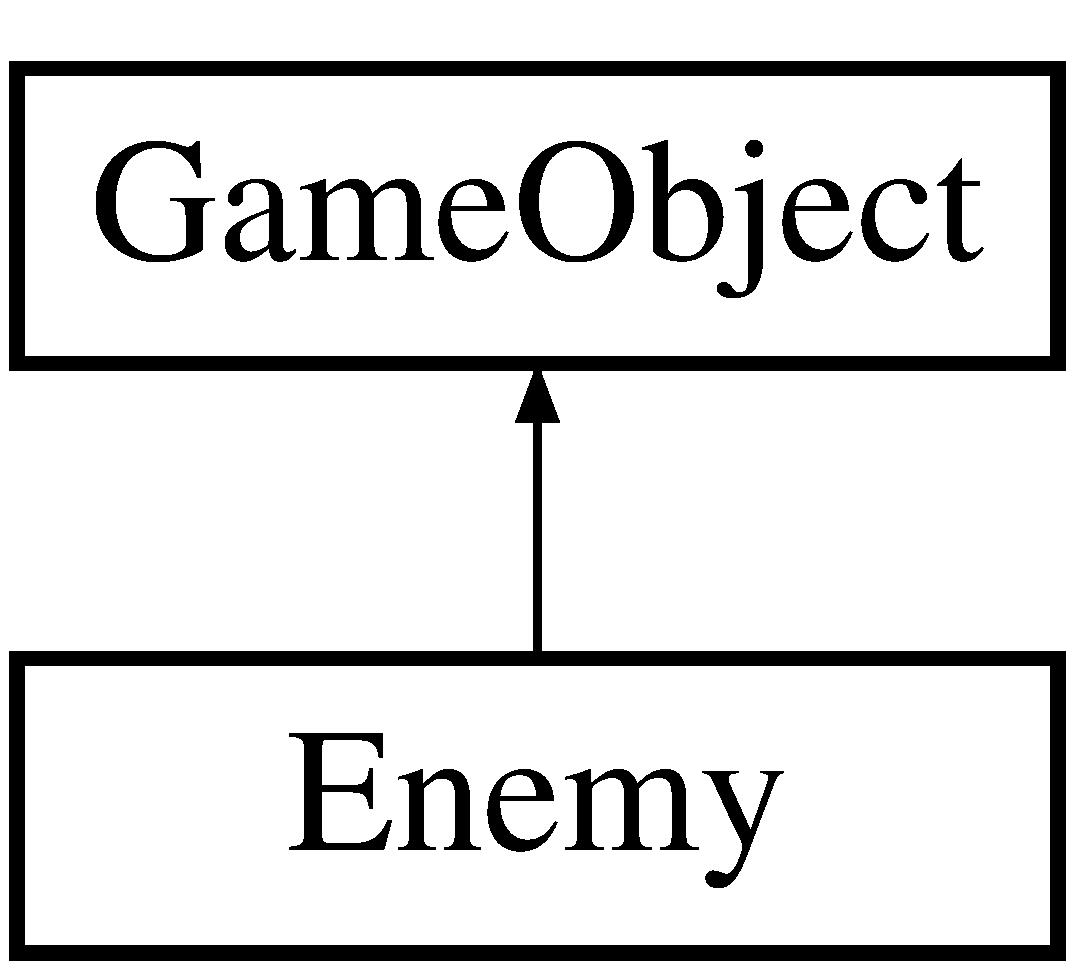
\includegraphics[height=2.000000cm]{class_enemy}
\end{center}
\end{figure}
\subsection*{Public Types}
\begin{DoxyCompactItemize}
\item 
enum \mbox{\hyperlink{class_enemy_ae6c971b1c4da1335dfd6542dea6efecb}{E\+N\+E\+M\+Y\+\_\+\+T\+Y\+PE}} \{ \mbox{\hyperlink{class_enemy_ae6c971b1c4da1335dfd6542dea6efecbaa842e3e91308061ef257ce005b8426be}{S\+Q\+U\+ID}}, 
\mbox{\hyperlink{class_enemy_ae6c971b1c4da1335dfd6542dea6efecba57bf1820642551b8e2e260613b8dce50}{G\+H\+O\+ST}}, 
\mbox{\hyperlink{class_enemy_ae6c971b1c4da1335dfd6542dea6efecbaaf4e9f1052313811c191ab9db18005e9}{A\+L\+I\+EN}}
 \}
\end{DoxyCompactItemize}
\subsection*{Public Member Functions}
\begin{DoxyCompactItemize}
\item 
\mbox{\hyperlink{class_enemy_ac14d80ce4f82c579e5fe1406e5bb25fa}{Enemy}} (S\+D\+L\+\_\+\+Renderer $\ast$renderer, int x, int y, \mbox{\hyperlink{class_enemy_ae6c971b1c4da1335dfd6542dea6efecb}{E\+N\+E\+M\+Y\+\_\+\+T\+Y\+PE}} type)
\item 
\mbox{\hyperlink{class_enemy_ac0eec4755e28c02688065f9657150ac3}{$\sim$\+Enemy}} ()
\item 
void \mbox{\hyperlink{class_enemy_adcde768475970dae1e4c3e76fb59bc46}{Logic}} ()
\end{DoxyCompactItemize}
\subsection*{Additional Inherited Members}


\subsection{Member Enumeration Documentation}
\mbox{\Hypertarget{class_enemy_ae6c971b1c4da1335dfd6542dea6efecb}\label{class_enemy_ae6c971b1c4da1335dfd6542dea6efecb}} 
\index{Enemy@{Enemy}!E\+N\+E\+M\+Y\+\_\+\+T\+Y\+PE@{E\+N\+E\+M\+Y\+\_\+\+T\+Y\+PE}}
\index{E\+N\+E\+M\+Y\+\_\+\+T\+Y\+PE@{E\+N\+E\+M\+Y\+\_\+\+T\+Y\+PE}!Enemy@{Enemy}}
\subsubsection{\texorpdfstring{E\+N\+E\+M\+Y\+\_\+\+T\+Y\+PE}{ENEMY\_TYPE}}
{\footnotesize\ttfamily enum \mbox{\hyperlink{class_enemy_ae6c971b1c4da1335dfd6542dea6efecb}{Enemy\+::\+E\+N\+E\+M\+Y\+\_\+\+T\+Y\+PE}}}

\begin{DoxyEnumFields}{Enumerator}
\raisebox{\heightof{T}}[0pt][0pt]{\index{S\+Q\+U\+ID@{S\+Q\+U\+ID}!Enemy@{Enemy}}\index{Enemy@{Enemy}!S\+Q\+U\+ID@{S\+Q\+U\+ID}}}\mbox{\Hypertarget{class_enemy_ae6c971b1c4da1335dfd6542dea6efecbaa842e3e91308061ef257ce005b8426be}\label{class_enemy_ae6c971b1c4da1335dfd6542dea6efecbaa842e3e91308061ef257ce005b8426be}} 
S\+Q\+U\+ID&\\
\hline

\raisebox{\heightof{T}}[0pt][0pt]{\index{G\+H\+O\+ST@{G\+H\+O\+ST}!Enemy@{Enemy}}\index{Enemy@{Enemy}!G\+H\+O\+ST@{G\+H\+O\+ST}}}\mbox{\Hypertarget{class_enemy_ae6c971b1c4da1335dfd6542dea6efecba57bf1820642551b8e2e260613b8dce50}\label{class_enemy_ae6c971b1c4da1335dfd6542dea6efecba57bf1820642551b8e2e260613b8dce50}} 
G\+H\+O\+ST&\\
\hline

\raisebox{\heightof{T}}[0pt][0pt]{\index{A\+L\+I\+EN@{A\+L\+I\+EN}!Enemy@{Enemy}}\index{Enemy@{Enemy}!A\+L\+I\+EN@{A\+L\+I\+EN}}}\mbox{\Hypertarget{class_enemy_ae6c971b1c4da1335dfd6542dea6efecbaaf4e9f1052313811c191ab9db18005e9}\label{class_enemy_ae6c971b1c4da1335dfd6542dea6efecbaaf4e9f1052313811c191ab9db18005e9}} 
A\+L\+I\+EN&\\
\hline

\end{DoxyEnumFields}


\subsection{Constructor \& Destructor Documentation}
\mbox{\Hypertarget{class_enemy_ac14d80ce4f82c579e5fe1406e5bb25fa}\label{class_enemy_ac14d80ce4f82c579e5fe1406e5bb25fa}} 
\index{Enemy@{Enemy}!Enemy@{Enemy}}
\index{Enemy@{Enemy}!Enemy@{Enemy}}
\subsubsection{\texorpdfstring{Enemy()}{Enemy()}}
{\footnotesize\ttfamily Enemy\+::\+Enemy (\begin{DoxyParamCaption}\item[{S\+D\+L\+\_\+\+Renderer $\ast$}]{renderer,  }\item[{int}]{x,  }\item[{int}]{y,  }\item[{\mbox{\hyperlink{class_enemy_ae6c971b1c4da1335dfd6542dea6efecb}{E\+N\+E\+M\+Y\+\_\+\+T\+Y\+PE}}}]{type }\end{DoxyParamCaption})}

\mbox{\Hypertarget{class_enemy_ac0eec4755e28c02688065f9657150ac3}\label{class_enemy_ac0eec4755e28c02688065f9657150ac3}} 
\index{Enemy@{Enemy}!````~Enemy@{$\sim$\+Enemy}}
\index{````~Enemy@{$\sim$\+Enemy}!Enemy@{Enemy}}
\subsubsection{\texorpdfstring{$\sim$\+Enemy()}{~Enemy()}}
{\footnotesize\ttfamily Enemy\+::$\sim$\+Enemy (\begin{DoxyParamCaption}{ }\end{DoxyParamCaption})}



\subsection{Member Function Documentation}
\mbox{\Hypertarget{class_enemy_adcde768475970dae1e4c3e76fb59bc46}\label{class_enemy_adcde768475970dae1e4c3e76fb59bc46}} 
\index{Enemy@{Enemy}!Logic@{Logic}}
\index{Logic@{Logic}!Enemy@{Enemy}}
\subsubsection{\texorpdfstring{Logic()}{Logic()}}
{\footnotesize\ttfamily void Enemy\+::\+Logic (\begin{DoxyParamCaption}{ }\end{DoxyParamCaption})\hspace{0.3cm}{\ttfamily [virtual]}}



Reimplemented from \mbox{\hyperlink{class_game_object_a79510ffc77339fe850491dce9f580fa9}{Game\+Object}}.



The documentation for this class was generated from the following files\+:\begin{DoxyCompactItemize}
\item 
Eksamen\+Base/\+Game\+Objects/\mbox{\hyperlink{_enemy_8h}{Enemy.\+h}}\item 
Eksamen\+Base/\+Game\+Objects/\mbox{\hyperlink{_enemy_8cpp}{Enemy.\+cpp}}\end{DoxyCompactItemize}

\hypertarget{class_enemy_attack}{}\section{Enemy\+Attack Class Reference}
\label{class_enemy_attack}\index{Enemy\+Attack@{Enemy\+Attack}}


{\ttfamily \#include $<$Enemy\+Attack.\+h$>$}

Inheritance diagram for Enemy\+Attack\+:\begin{figure}[H]
\begin{center}
\leavevmode
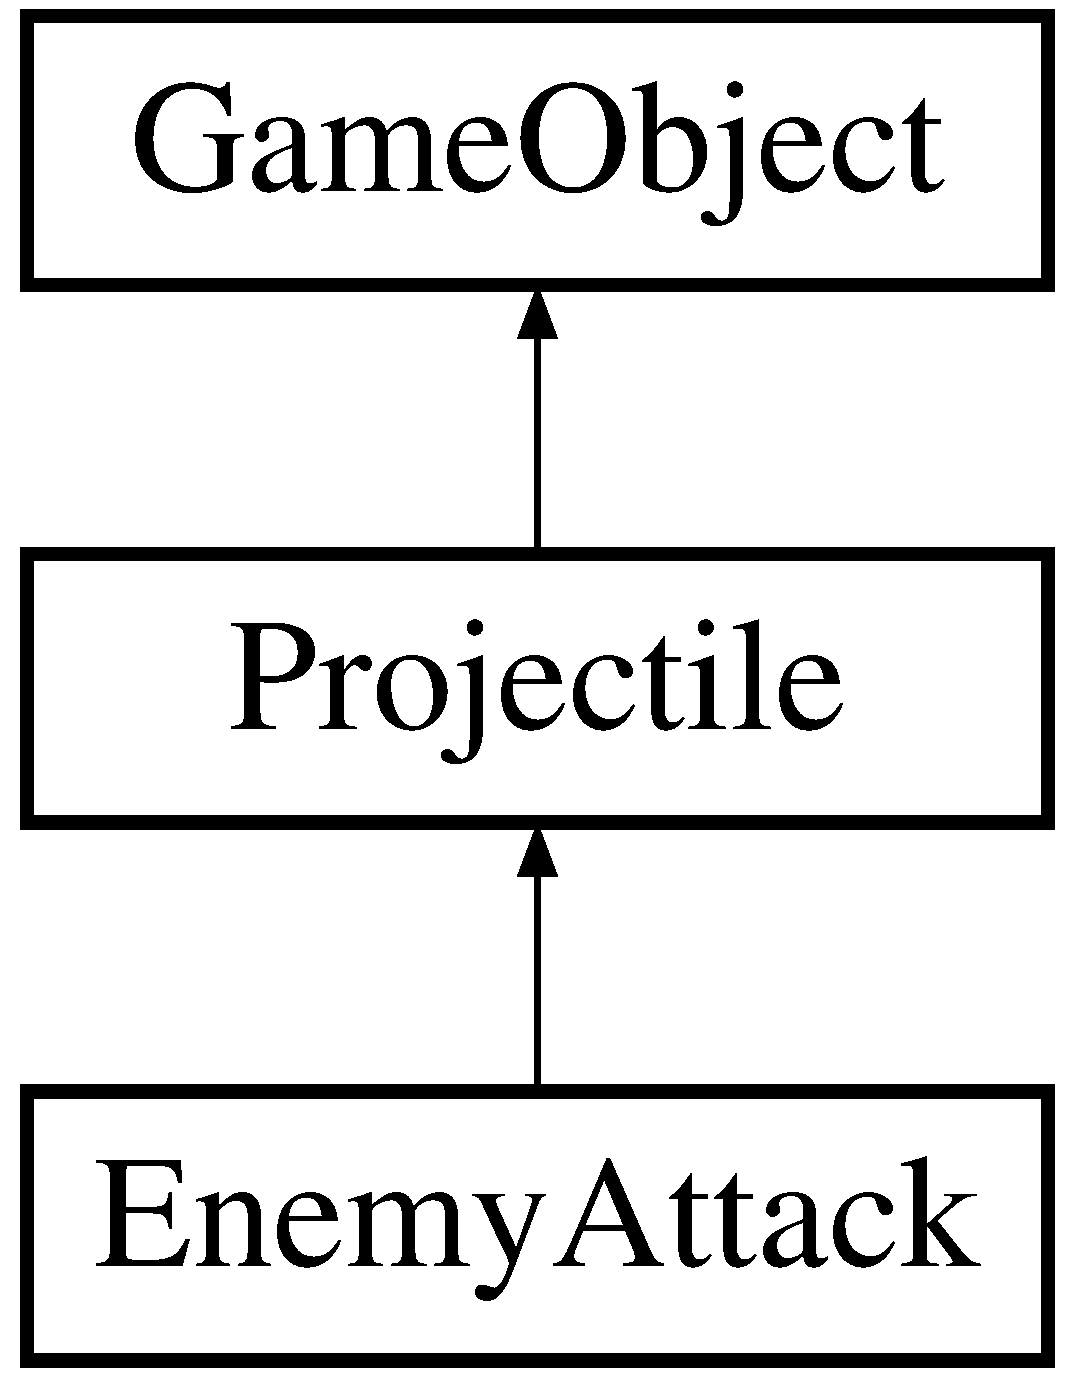
\includegraphics[height=3.000000cm]{class_enemy_attack}
\end{center}
\end{figure}
\subsection*{Public Member Functions}
\begin{DoxyCompactItemize}
\item 
\mbox{\hyperlink{class_enemy_attack_a169f1749ce1126148be5ec7d94554e45}{Enemy\+Attack}} (S\+D\+L\+\_\+\+Renderer $\ast$renderer, int x, int y)
\item 
\mbox{\hyperlink{class_enemy_attack_abc5fbac33c1c8d61ab70e4a480980c77}{$\sim$\+Enemy\+Attack}} ()
\item 
void \mbox{\hyperlink{class_enemy_attack_a2f735b2cbf13787217a5daed7ff8f7a4}{Logic}} ()
\end{DoxyCompactItemize}
\subsection*{Additional Inherited Members}


\subsection{Constructor \& Destructor Documentation}
\mbox{\Hypertarget{class_enemy_attack_a169f1749ce1126148be5ec7d94554e45}\label{class_enemy_attack_a169f1749ce1126148be5ec7d94554e45}} 
\index{Enemy\+Attack@{Enemy\+Attack}!Enemy\+Attack@{Enemy\+Attack}}
\index{Enemy\+Attack@{Enemy\+Attack}!Enemy\+Attack@{Enemy\+Attack}}
\subsubsection{\texorpdfstring{Enemy\+Attack()}{EnemyAttack()}}
{\footnotesize\ttfamily Enemy\+Attack\+::\+Enemy\+Attack (\begin{DoxyParamCaption}\item[{S\+D\+L\+\_\+\+Renderer $\ast$}]{renderer,  }\item[{int}]{x,  }\item[{int}]{y }\end{DoxyParamCaption})}

\mbox{\Hypertarget{class_enemy_attack_abc5fbac33c1c8d61ab70e4a480980c77}\label{class_enemy_attack_abc5fbac33c1c8d61ab70e4a480980c77}} 
\index{Enemy\+Attack@{Enemy\+Attack}!````~Enemy\+Attack@{$\sim$\+Enemy\+Attack}}
\index{````~Enemy\+Attack@{$\sim$\+Enemy\+Attack}!Enemy\+Attack@{Enemy\+Attack}}
\subsubsection{\texorpdfstring{$\sim$\+Enemy\+Attack()}{~EnemyAttack()}}
{\footnotesize\ttfamily Enemy\+Attack\+::$\sim$\+Enemy\+Attack (\begin{DoxyParamCaption}{ }\end{DoxyParamCaption})}



\subsection{Member Function Documentation}
\mbox{\Hypertarget{class_enemy_attack_a2f735b2cbf13787217a5daed7ff8f7a4}\label{class_enemy_attack_a2f735b2cbf13787217a5daed7ff8f7a4}} 
\index{Enemy\+Attack@{Enemy\+Attack}!Logic@{Logic}}
\index{Logic@{Logic}!Enemy\+Attack@{Enemy\+Attack}}
\subsubsection{\texorpdfstring{Logic()}{Logic()}}
{\footnotesize\ttfamily void Enemy\+Attack\+::\+Logic (\begin{DoxyParamCaption}{ }\end{DoxyParamCaption})\hspace{0.3cm}{\ttfamily [virtual]}}



Reimplemented from \mbox{\hyperlink{class_game_object_a79510ffc77339fe850491dce9f580fa9}{Game\+Object}}.



The documentation for this class was generated from the following files\+:\begin{DoxyCompactItemize}
\item 
Eksamen\+Base/\+Game\+Objects/\mbox{\hyperlink{_enemy_attack_8h}{Enemy\+Attack.\+h}}\item 
Eksamen\+Base/\+Game\+Objects/\mbox{\hyperlink{_enemy_attack_8cpp}{Enemy\+Attack.\+cpp}}\end{DoxyCompactItemize}

\hypertarget{class_game_handler}{}\section{Game\+Handler Class Reference}
\label{class_game_handler}\index{Game\+Handler@{Game\+Handler}}


{\ttfamily \#include $<$Game\+Handler.\+h$>$}

\subsection*{Public Member Functions}
\begin{DoxyCompactItemize}
\item 
\mbox{\hyperlink{class_game_handler_ad016ced8da1d660009e014a9aeb833da}{Game\+Handler}} ()
\item 
\mbox{\hyperlink{class_game_handler_a37e9acdced835f48a2bb2a00cb322635}{$\sim$\+Game\+Handler}} ()
\begin{DoxyCompactList}\small\item\em \mbox{\hyperlink{class_game_handler}{Game\+Handler}} destructor \end{DoxyCompactList}\item 
void \mbox{\hyperlink{class_game_handler_aba984ea50d3ce52070950c5aa24e0d7f}{Init}} ()
\begin{DoxyCompactList}\small\item\em Inits S\+DL \end{DoxyCompactList}\end{DoxyCompactItemize}
\subsection*{Static Public Member Functions}
\begin{DoxyCompactItemize}
\item 
static double \mbox{\hyperlink{class_game_handler_aebe798f7fee6c05c05bec6540f240238}{get\+Delta\+Time}} ()
\begin{DoxyCompactList}\small\item\em Returns the deltatime \end{DoxyCompactList}\end{DoxyCompactItemize}
\subsection*{Static Public Attributes}
\begin{DoxyCompactItemize}
\item 
static const int \mbox{\hyperlink{class_game_handler_a9ae6b1b8478a4bc1928f07d5e52d0b95}{S\+C\+R\+E\+E\+N\+\_\+\+W\+I\+D\+TH}} = 640
\item 
static const int \mbox{\hyperlink{class_game_handler_af09c16007a8cb793fa21dd5fb5d31201}{S\+C\+R\+E\+E\+N\+\_\+\+H\+E\+I\+G\+HT}} = 480
\item 
static int \mbox{\hyperlink{class_game_handler_a985aa228815f283446ce0f354f513e80}{score}} = 0
\item 
static int \mbox{\hyperlink{class_game_handler_a0076f4fe9cad55a986a899bd14b97061}{high\+Score}} = 0
\item 
static int \mbox{\hyperlink{class_game_handler_a534070acd7b75bb0d08f73da3b0afb68}{level}} = 1
\end{DoxyCompactItemize}


\subsection{Constructor \& Destructor Documentation}
\mbox{\Hypertarget{class_game_handler_ad016ced8da1d660009e014a9aeb833da}\label{class_game_handler_ad016ced8da1d660009e014a9aeb833da}} 
\index{Game\+Handler@{Game\+Handler}!Game\+Handler@{Game\+Handler}}
\index{Game\+Handler@{Game\+Handler}!Game\+Handler@{Game\+Handler}}
\subsubsection{\texorpdfstring{Game\+Handler()}{GameHandler()}}
{\footnotesize\ttfamily Game\+Handler\+::\+Game\+Handler (\begin{DoxyParamCaption}{ }\end{DoxyParamCaption})}

\mbox{\Hypertarget{class_game_handler_a37e9acdced835f48a2bb2a00cb322635}\label{class_game_handler_a37e9acdced835f48a2bb2a00cb322635}} 
\index{Game\+Handler@{Game\+Handler}!````~Game\+Handler@{$\sim$\+Game\+Handler}}
\index{````~Game\+Handler@{$\sim$\+Game\+Handler}!Game\+Handler@{Game\+Handler}}
\subsubsection{\texorpdfstring{$\sim$\+Game\+Handler()}{~GameHandler()}}
{\footnotesize\ttfamily Game\+Handler\+::$\sim$\+Game\+Handler (\begin{DoxyParamCaption}{ }\end{DoxyParamCaption})}



\mbox{\hyperlink{class_game_handler}{Game\+Handler}} destructor 



\subsection{Member Function Documentation}
\mbox{\Hypertarget{class_game_handler_aebe798f7fee6c05c05bec6540f240238}\label{class_game_handler_aebe798f7fee6c05c05bec6540f240238}} 
\index{Game\+Handler@{Game\+Handler}!get\+Delta\+Time@{get\+Delta\+Time}}
\index{get\+Delta\+Time@{get\+Delta\+Time}!Game\+Handler@{Game\+Handler}}
\subsubsection{\texorpdfstring{get\+Delta\+Time()}{getDeltaTime()}}
{\footnotesize\ttfamily double Game\+Handler\+::get\+Delta\+Time (\begin{DoxyParamCaption}{ }\end{DoxyParamCaption})\hspace{0.3cm}{\ttfamily [static]}}



Returns the deltatime 

\begin{DoxyReturn}{Returns}

\end{DoxyReturn}
\mbox{\Hypertarget{class_game_handler_aba984ea50d3ce52070950c5aa24e0d7f}\label{class_game_handler_aba984ea50d3ce52070950c5aa24e0d7f}} 
\index{Game\+Handler@{Game\+Handler}!Init@{Init}}
\index{Init@{Init}!Game\+Handler@{Game\+Handler}}
\subsubsection{\texorpdfstring{Init()}{Init()}}
{\footnotesize\ttfamily void Game\+Handler\+::\+Init (\begin{DoxyParamCaption}{ }\end{DoxyParamCaption})}



Inits S\+DL 



\subsection{Member Data Documentation}
\mbox{\Hypertarget{class_game_handler_a0076f4fe9cad55a986a899bd14b97061}\label{class_game_handler_a0076f4fe9cad55a986a899bd14b97061}} 
\index{Game\+Handler@{Game\+Handler}!high\+Score@{high\+Score}}
\index{high\+Score@{high\+Score}!Game\+Handler@{Game\+Handler}}
\subsubsection{\texorpdfstring{high\+Score}{highScore}}
{\footnotesize\ttfamily int Game\+Handler\+::high\+Score = 0\hspace{0.3cm}{\ttfamily [static]}}

\mbox{\Hypertarget{class_game_handler_a534070acd7b75bb0d08f73da3b0afb68}\label{class_game_handler_a534070acd7b75bb0d08f73da3b0afb68}} 
\index{Game\+Handler@{Game\+Handler}!level@{level}}
\index{level@{level}!Game\+Handler@{Game\+Handler}}
\subsubsection{\texorpdfstring{level}{level}}
{\footnotesize\ttfamily int Game\+Handler\+::level = 1\hspace{0.3cm}{\ttfamily [static]}}

\mbox{\Hypertarget{class_game_handler_a985aa228815f283446ce0f354f513e80}\label{class_game_handler_a985aa228815f283446ce0f354f513e80}} 
\index{Game\+Handler@{Game\+Handler}!score@{score}}
\index{score@{score}!Game\+Handler@{Game\+Handler}}
\subsubsection{\texorpdfstring{score}{score}}
{\footnotesize\ttfamily int Game\+Handler\+::score = 0\hspace{0.3cm}{\ttfamily [static]}}

\mbox{\Hypertarget{class_game_handler_af09c16007a8cb793fa21dd5fb5d31201}\label{class_game_handler_af09c16007a8cb793fa21dd5fb5d31201}} 
\index{Game\+Handler@{Game\+Handler}!S\+C\+R\+E\+E\+N\+\_\+\+H\+E\+I\+G\+HT@{S\+C\+R\+E\+E\+N\+\_\+\+H\+E\+I\+G\+HT}}
\index{S\+C\+R\+E\+E\+N\+\_\+\+H\+E\+I\+G\+HT@{S\+C\+R\+E\+E\+N\+\_\+\+H\+E\+I\+G\+HT}!Game\+Handler@{Game\+Handler}}
\subsubsection{\texorpdfstring{S\+C\+R\+E\+E\+N\+\_\+\+H\+E\+I\+G\+HT}{SCREEN\_HEIGHT}}
{\footnotesize\ttfamily const int Game\+Handler\+::\+S\+C\+R\+E\+E\+N\+\_\+\+H\+E\+I\+G\+HT = 480\hspace{0.3cm}{\ttfamily [static]}}

\mbox{\Hypertarget{class_game_handler_a9ae6b1b8478a4bc1928f07d5e52d0b95}\label{class_game_handler_a9ae6b1b8478a4bc1928f07d5e52d0b95}} 
\index{Game\+Handler@{Game\+Handler}!S\+C\+R\+E\+E\+N\+\_\+\+W\+I\+D\+TH@{S\+C\+R\+E\+E\+N\+\_\+\+W\+I\+D\+TH}}
\index{S\+C\+R\+E\+E\+N\+\_\+\+W\+I\+D\+TH@{S\+C\+R\+E\+E\+N\+\_\+\+W\+I\+D\+TH}!Game\+Handler@{Game\+Handler}}
\subsubsection{\texorpdfstring{S\+C\+R\+E\+E\+N\+\_\+\+W\+I\+D\+TH}{SCREEN\_WIDTH}}
{\footnotesize\ttfamily const int Game\+Handler\+::\+S\+C\+R\+E\+E\+N\+\_\+\+W\+I\+D\+TH = 640\hspace{0.3cm}{\ttfamily [static]}}



The documentation for this class was generated from the following files\+:\begin{DoxyCompactItemize}
\item 
Eksamen\+Base/\+Handlers/\mbox{\hyperlink{_game_handler_8h}{Game\+Handler.\+h}}\item 
Eksamen\+Base/\+Handlers/\mbox{\hyperlink{_game_handler_8cpp}{Game\+Handler.\+cpp}}\end{DoxyCompactItemize}

\hypertarget{class_game_object}{}\section{Game\+Object Class Reference}
\label{class_game_object}\index{Game\+Object@{Game\+Object}}


{\ttfamily \#include $<$Game\+Object.\+h$>$}

Inheritance diagram for Game\+Object\+:\begin{figure}[H]
\begin{center}
\leavevmode
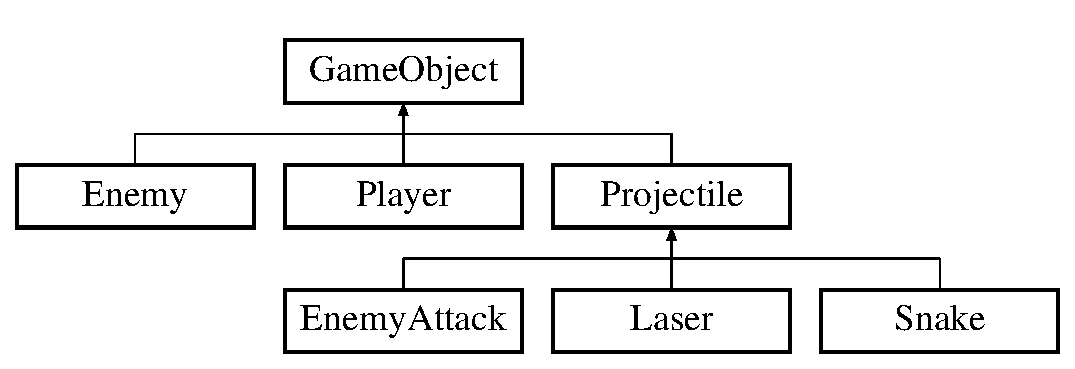
\includegraphics[height=3.000000cm]{class_game_object}
\end{center}
\end{figure}
\subsection*{Classes}
\begin{DoxyCompactItemize}
\item 
struct \mbox{\hyperlink{struct_game_object_1_1_vector2_d}{Vector2D}}
\end{DoxyCompactItemize}
\subsection*{Public Member Functions}
\begin{DoxyCompactItemize}
\item 
\mbox{\hyperlink{class_game_object_a0b60783781874241ad26049ad968a78b}{Game\+Object}} (S\+D\+L\+\_\+\+Renderer $\ast$renderer)
\item 
\mbox{\hyperlink{class_game_object_ab82dfdb656f9051c0587e6593b2dda97}{$\sim$\+Game\+Object}} ()
\item 
virtual void \mbox{\hyperlink{class_game_object_a79510ffc77339fe850491dce9f580fa9}{Logic}} ()
\item 
virtual void \mbox{\hyperlink{class_game_object_ad3ac1deac50048cf7a1a19eb0e61ad26}{Draw}} ()
\item 
virtual void \mbox{\hyperlink{class_game_object_a430742cf91abb99337c556c88bef880a}{Input}} ()
\item 
int \mbox{\hyperlink{class_game_object_a13b96d5c268bca096f8e3a3e85d35732}{get\+Hp}} () const
\begin{DoxyCompactList}\small\item\em Returns HP \end{DoxyCompactList}\item 
void \mbox{\hyperlink{class_game_object_a7aa67e2bbfd37af89d86df0b030b5a81}{set\+Hp}} (int hp)
\begin{DoxyCompactList}\small\item\em Sets HP \end{DoxyCompactList}\end{DoxyCompactItemize}
\subsection*{Public Attributes}
\begin{DoxyCompactItemize}
\item 
S\+D\+L\+\_\+\+Rect \mbox{\hyperlink{class_game_object_af6009d73be98a4bd54272d06b50f2eac}{position}}
\item 
std\+::string \mbox{\hyperlink{class_game_object_a66891b8bfd67373dde0155ae7808bbb4}{tag}}
\item 
int \mbox{\hyperlink{class_game_object_a98291c60da12d9036e1ad24cfebcf6b3}{id}}
\end{DoxyCompactItemize}
\subsection*{Protected Attributes}
\begin{DoxyCompactItemize}
\item 
S\+D\+L\+\_\+\+Texture $\ast$ \mbox{\hyperlink{class_game_object_a5202d5d5df1813c567fb344617250b42}{m\+\_\+def\+Texture}}
\item 
S\+D\+L\+\_\+\+Texture $\ast$ \mbox{\hyperlink{class_game_object_aa89e916d62813d047b054c0c9cf97559}{m\+\_\+secondary\+Texture}}
\item 
S\+D\+L\+\_\+\+Renderer $\ast$ \mbox{\hyperlink{class_game_object_a2be93417ea72201ce5edc093167b2f68}{m\+\_\+renderer}}
\item 
\mbox{\hyperlink{struct_game_object_1_1_vector2_d}{Vector2D}} \mbox{\hyperlink{class_game_object_ac27549efb645f7c924d6604e318877bf}{m\+\_\+velocity}}
\item 
\mbox{\hyperlink{struct_game_object_1_1_vector2_d}{Vector2D}} \mbox{\hyperlink{class_game_object_a934563079577e8f20b597e23ae40ec20}{m\+\_\+acceleration}}
\item 
float \mbox{\hyperlink{class_game_object_a82b60a9ea631d253434ba8683ee69370}{m\+\_\+de\+Acceleration}}
\item 
float \mbox{\hyperlink{class_game_object_a6a2eccbbf7974ae9d76e58f4f5b899ac}{m\+\_\+acceleration\+Value}}
\item 
float \mbox{\hyperlink{class_game_object_a13670cbe19b2daaedbd696a3495bf598}{m\+\_\+max\+Speed}} = .\+5f
\item 
int \mbox{\hyperlink{class_game_object_a26687f9a79576969707c47f5562b7037}{m\+\_\+hp}}
\end{DoxyCompactItemize}


\subsection{Constructor \& Destructor Documentation}
\mbox{\Hypertarget{class_game_object_a0b60783781874241ad26049ad968a78b}\label{class_game_object_a0b60783781874241ad26049ad968a78b}} 
\index{Game\+Object@{Game\+Object}!Game\+Object@{Game\+Object}}
\index{Game\+Object@{Game\+Object}!Game\+Object@{Game\+Object}}
\subsubsection{\texorpdfstring{Game\+Object()}{GameObject()}}
{\footnotesize\ttfamily Game\+Object\+::\+Game\+Object (\begin{DoxyParamCaption}\item[{S\+D\+L\+\_\+\+Renderer $\ast$}]{renderer }\end{DoxyParamCaption})}

\mbox{\Hypertarget{class_game_object_ab82dfdb656f9051c0587e6593b2dda97}\label{class_game_object_ab82dfdb656f9051c0587e6593b2dda97}} 
\index{Game\+Object@{Game\+Object}!````~Game\+Object@{$\sim$\+Game\+Object}}
\index{````~Game\+Object@{$\sim$\+Game\+Object}!Game\+Object@{Game\+Object}}
\subsubsection{\texorpdfstring{$\sim$\+Game\+Object()}{~GameObject()}}
{\footnotesize\ttfamily Game\+Object\+::$\sim$\+Game\+Object (\begin{DoxyParamCaption}{ }\end{DoxyParamCaption})}



\subsection{Member Function Documentation}
\mbox{\Hypertarget{class_game_object_ad3ac1deac50048cf7a1a19eb0e61ad26}\label{class_game_object_ad3ac1deac50048cf7a1a19eb0e61ad26}} 
\index{Game\+Object@{Game\+Object}!Draw@{Draw}}
\index{Draw@{Draw}!Game\+Object@{Game\+Object}}
\subsubsection{\texorpdfstring{Draw()}{Draw()}}
{\footnotesize\ttfamily void Game\+Object\+::\+Draw (\begin{DoxyParamCaption}{ }\end{DoxyParamCaption})\hspace{0.3cm}{\ttfamily [virtual]}}

\mbox{\Hypertarget{class_game_object_a13b96d5c268bca096f8e3a3e85d35732}\label{class_game_object_a13b96d5c268bca096f8e3a3e85d35732}} 
\index{Game\+Object@{Game\+Object}!get\+Hp@{get\+Hp}}
\index{get\+Hp@{get\+Hp}!Game\+Object@{Game\+Object}}
\subsubsection{\texorpdfstring{get\+Hp()}{getHp()}}
{\footnotesize\ttfamily int Game\+Object\+::get\+Hp (\begin{DoxyParamCaption}{ }\end{DoxyParamCaption}) const}



Returns HP 

\begin{DoxyReturn}{Returns}

\end{DoxyReturn}
\mbox{\Hypertarget{class_game_object_a430742cf91abb99337c556c88bef880a}\label{class_game_object_a430742cf91abb99337c556c88bef880a}} 
\index{Game\+Object@{Game\+Object}!Input@{Input}}
\index{Input@{Input}!Game\+Object@{Game\+Object}}
\subsubsection{\texorpdfstring{Input()}{Input()}}
{\footnotesize\ttfamily void Game\+Object\+::\+Input (\begin{DoxyParamCaption}{ }\end{DoxyParamCaption})\hspace{0.3cm}{\ttfamily [virtual]}}



Reimplemented in \mbox{\hyperlink{class_enemy_ad4958e67a70c706e37a80b285ac89854}{Enemy}}, and \mbox{\hyperlink{class_player_a65a76094cff6f149d5847d2110fe443d}{Player}}.

\mbox{\Hypertarget{class_game_object_a79510ffc77339fe850491dce9f580fa9}\label{class_game_object_a79510ffc77339fe850491dce9f580fa9}} 
\index{Game\+Object@{Game\+Object}!Logic@{Logic}}
\index{Logic@{Logic}!Game\+Object@{Game\+Object}}
\subsubsection{\texorpdfstring{Logic()}{Logic()}}
{\footnotesize\ttfamily void Game\+Object\+::\+Logic (\begin{DoxyParamCaption}{ }\end{DoxyParamCaption})\hspace{0.3cm}{\ttfamily [virtual]}}



Reimplemented in \mbox{\hyperlink{class_projectile_a871e265207d2bf2d5180152a7acf2d40}{Projectile}}, \mbox{\hyperlink{class_enemy_adcde768475970dae1e4c3e76fb59bc46}{Enemy}}, \mbox{\hyperlink{class_snake_a1f01e21a73734f9c0d701ec02a9d2e41}{Snake}}, \mbox{\hyperlink{class_enemy_attack_a2f735b2cbf13787217a5daed7ff8f7a4}{Enemy\+Attack}}, \mbox{\hyperlink{class_laser_a1f2135281ecc1b318357633f4e7dd34c}{Laser}}, and \mbox{\hyperlink{class_player_ae30c8d49de94ee8c73ed6ab6315a2854}{Player}}.

\mbox{\Hypertarget{class_game_object_a7aa67e2bbfd37af89d86df0b030b5a81}\label{class_game_object_a7aa67e2bbfd37af89d86df0b030b5a81}} 
\index{Game\+Object@{Game\+Object}!set\+Hp@{set\+Hp}}
\index{set\+Hp@{set\+Hp}!Game\+Object@{Game\+Object}}
\subsubsection{\texorpdfstring{set\+Hp()}{setHp()}}
{\footnotesize\ttfamily void Game\+Object\+::set\+Hp (\begin{DoxyParamCaption}\item[{int}]{hp }\end{DoxyParamCaption})}



Sets HP 


\begin{DoxyParams}{Parameters}
{\em hp} & \\
\hline
\end{DoxyParams}


\subsection{Member Data Documentation}
\mbox{\Hypertarget{class_game_object_a98291c60da12d9036e1ad24cfebcf6b3}\label{class_game_object_a98291c60da12d9036e1ad24cfebcf6b3}} 
\index{Game\+Object@{Game\+Object}!id@{id}}
\index{id@{id}!Game\+Object@{Game\+Object}}
\subsubsection{\texorpdfstring{id}{id}}
{\footnotesize\ttfamily int Game\+Object\+::id}

\mbox{\Hypertarget{class_game_object_a934563079577e8f20b597e23ae40ec20}\label{class_game_object_a934563079577e8f20b597e23ae40ec20}} 
\index{Game\+Object@{Game\+Object}!m\+\_\+acceleration@{m\+\_\+acceleration}}
\index{m\+\_\+acceleration@{m\+\_\+acceleration}!Game\+Object@{Game\+Object}}
\subsubsection{\texorpdfstring{m\+\_\+acceleration}{m\_acceleration}}
{\footnotesize\ttfamily \mbox{\hyperlink{struct_game_object_1_1_vector2_d}{Vector2D}} Game\+Object\+::m\+\_\+acceleration\hspace{0.3cm}{\ttfamily [protected]}}

\mbox{\Hypertarget{class_game_object_a6a2eccbbf7974ae9d76e58f4f5b899ac}\label{class_game_object_a6a2eccbbf7974ae9d76e58f4f5b899ac}} 
\index{Game\+Object@{Game\+Object}!m\+\_\+acceleration\+Value@{m\+\_\+acceleration\+Value}}
\index{m\+\_\+acceleration\+Value@{m\+\_\+acceleration\+Value}!Game\+Object@{Game\+Object}}
\subsubsection{\texorpdfstring{m\+\_\+acceleration\+Value}{m\_accelerationValue}}
{\footnotesize\ttfamily float Game\+Object\+::m\+\_\+acceleration\+Value\hspace{0.3cm}{\ttfamily [protected]}}

\mbox{\Hypertarget{class_game_object_a82b60a9ea631d253434ba8683ee69370}\label{class_game_object_a82b60a9ea631d253434ba8683ee69370}} 
\index{Game\+Object@{Game\+Object}!m\+\_\+de\+Acceleration@{m\+\_\+de\+Acceleration}}
\index{m\+\_\+de\+Acceleration@{m\+\_\+de\+Acceleration}!Game\+Object@{Game\+Object}}
\subsubsection{\texorpdfstring{m\+\_\+de\+Acceleration}{m\_deAcceleration}}
{\footnotesize\ttfamily float Game\+Object\+::m\+\_\+de\+Acceleration\hspace{0.3cm}{\ttfamily [protected]}}

\mbox{\Hypertarget{class_game_object_a5202d5d5df1813c567fb344617250b42}\label{class_game_object_a5202d5d5df1813c567fb344617250b42}} 
\index{Game\+Object@{Game\+Object}!m\+\_\+def\+Texture@{m\+\_\+def\+Texture}}
\index{m\+\_\+def\+Texture@{m\+\_\+def\+Texture}!Game\+Object@{Game\+Object}}
\subsubsection{\texorpdfstring{m\+\_\+def\+Texture}{m\_defTexture}}
{\footnotesize\ttfamily S\+D\+L\+\_\+\+Texture$\ast$ Game\+Object\+::m\+\_\+def\+Texture\hspace{0.3cm}{\ttfamily [protected]}}

\mbox{\Hypertarget{class_game_object_a26687f9a79576969707c47f5562b7037}\label{class_game_object_a26687f9a79576969707c47f5562b7037}} 
\index{Game\+Object@{Game\+Object}!m\+\_\+hp@{m\+\_\+hp}}
\index{m\+\_\+hp@{m\+\_\+hp}!Game\+Object@{Game\+Object}}
\subsubsection{\texorpdfstring{m\+\_\+hp}{m\_hp}}
{\footnotesize\ttfamily int Game\+Object\+::m\+\_\+hp\hspace{0.3cm}{\ttfamily [protected]}}

\mbox{\Hypertarget{class_game_object_a13670cbe19b2daaedbd696a3495bf598}\label{class_game_object_a13670cbe19b2daaedbd696a3495bf598}} 
\index{Game\+Object@{Game\+Object}!m\+\_\+max\+Speed@{m\+\_\+max\+Speed}}
\index{m\+\_\+max\+Speed@{m\+\_\+max\+Speed}!Game\+Object@{Game\+Object}}
\subsubsection{\texorpdfstring{m\+\_\+max\+Speed}{m\_maxSpeed}}
{\footnotesize\ttfamily float Game\+Object\+::m\+\_\+max\+Speed = .\+5f\hspace{0.3cm}{\ttfamily [protected]}}

\mbox{\Hypertarget{class_game_object_a2be93417ea72201ce5edc093167b2f68}\label{class_game_object_a2be93417ea72201ce5edc093167b2f68}} 
\index{Game\+Object@{Game\+Object}!m\+\_\+renderer@{m\+\_\+renderer}}
\index{m\+\_\+renderer@{m\+\_\+renderer}!Game\+Object@{Game\+Object}}
\subsubsection{\texorpdfstring{m\+\_\+renderer}{m\_renderer}}
{\footnotesize\ttfamily S\+D\+L\+\_\+\+Renderer$\ast$ Game\+Object\+::m\+\_\+renderer\hspace{0.3cm}{\ttfamily [protected]}}

\mbox{\Hypertarget{class_game_object_aa89e916d62813d047b054c0c9cf97559}\label{class_game_object_aa89e916d62813d047b054c0c9cf97559}} 
\index{Game\+Object@{Game\+Object}!m\+\_\+secondary\+Texture@{m\+\_\+secondary\+Texture}}
\index{m\+\_\+secondary\+Texture@{m\+\_\+secondary\+Texture}!Game\+Object@{Game\+Object}}
\subsubsection{\texorpdfstring{m\+\_\+secondary\+Texture}{m\_secondaryTexture}}
{\footnotesize\ttfamily S\+D\+L\+\_\+\+Texture$\ast$ Game\+Object\+::m\+\_\+secondary\+Texture\hspace{0.3cm}{\ttfamily [protected]}}

\mbox{\Hypertarget{class_game_object_ac27549efb645f7c924d6604e318877bf}\label{class_game_object_ac27549efb645f7c924d6604e318877bf}} 
\index{Game\+Object@{Game\+Object}!m\+\_\+velocity@{m\+\_\+velocity}}
\index{m\+\_\+velocity@{m\+\_\+velocity}!Game\+Object@{Game\+Object}}
\subsubsection{\texorpdfstring{m\+\_\+velocity}{m\_velocity}}
{\footnotesize\ttfamily \mbox{\hyperlink{struct_game_object_1_1_vector2_d}{Vector2D}} Game\+Object\+::m\+\_\+velocity\hspace{0.3cm}{\ttfamily [protected]}}

\mbox{\Hypertarget{class_game_object_af6009d73be98a4bd54272d06b50f2eac}\label{class_game_object_af6009d73be98a4bd54272d06b50f2eac}} 
\index{Game\+Object@{Game\+Object}!position@{position}}
\index{position@{position}!Game\+Object@{Game\+Object}}
\subsubsection{\texorpdfstring{position}{position}}
{\footnotesize\ttfamily S\+D\+L\+\_\+\+Rect Game\+Object\+::position}

\mbox{\Hypertarget{class_game_object_a66891b8bfd67373dde0155ae7808bbb4}\label{class_game_object_a66891b8bfd67373dde0155ae7808bbb4}} 
\index{Game\+Object@{Game\+Object}!tag@{tag}}
\index{tag@{tag}!Game\+Object@{Game\+Object}}
\subsubsection{\texorpdfstring{tag}{tag}}
{\footnotesize\ttfamily std\+::string Game\+Object\+::tag}



The documentation for this class was generated from the following files\+:\begin{DoxyCompactItemize}
\item 
Eksamen\+Base/\+Game\+Objects/\mbox{\hyperlink{_game_object_8h}{Game\+Object.\+h}}\item 
Eksamen\+Base/\+Game\+Objects/\mbox{\hyperlink{_game_object_8cpp}{Game\+Object.\+cpp}}\end{DoxyCompactItemize}

\hypertarget{class_game_objects_manager}{}\section{Game\+Objects\+Manager Class Reference}
\label{class_game_objects_manager}\index{Game\+Objects\+Manager@{Game\+Objects\+Manager}}


{\ttfamily \#include $<$Game\+Objects\+Manager.\+h$>$}

\subsection*{Public Member Functions}
\begin{DoxyCompactItemize}
\item 
\mbox{\hyperlink{class_game_objects_manager_abe5aece84355a01f2473b41217f28026}{$\sim$\+Game\+Objects\+Manager}} ()
\item 
void \mbox{\hyperlink{class_game_objects_manager_a20480f2dbcb4607aa74c75e6f4ddccdb}{Add}} (std\+::shared\+\_\+ptr$<$ \mbox{\hyperlink{class_game_object}{Game\+Object}} $>$ game\+Object)
\begin{DoxyCompactList}\small\item\em Adds the given gameobject to the list \end{DoxyCompactList}\item 
void \mbox{\hyperlink{class_game_objects_manager_a1aff7fa8c420de210baffadf2e2be703}{Remove}} (std\+::shared\+\_\+ptr$<$ \mbox{\hyperlink{class_game_object}{Game\+Object}} $>$ game\+Object)
\begin{DoxyCompactList}\small\item\em Removes the given gameobject \end{DoxyCompactList}\item 
std\+::vector$<$ std\+::shared\+\_\+ptr$<$ \mbox{\hyperlink{class_game_object}{Game\+Object}} $>$ $>$ $\ast$ \mbox{\hyperlink{class_game_objects_manager_a0f2728da34f1a966f2b7aa9a35f8e614}{Find}} (std\+::string tag)
\begin{DoxyCompactList}\small\item\em Retuns an array of gameobject with given tag T\+O\+DO\+:\+: Test it out, not sure if it works yo \end{DoxyCompactList}\item 
void \mbox{\hyperlink{class_game_objects_manager_a60c1378f98fbef5dc98c8fdd094ef3c9}{Draw}} ()
\begin{DoxyCompactList}\small\item\em Draws all of the gameobject \end{DoxyCompactList}\item 
void \mbox{\hyperlink{class_game_objects_manager_a9f5ca8d981a423e9c5ab56978a1cd99e}{Input}} ()
\begin{DoxyCompactList}\small\item\em Handles the input for all the gameobjects \end{DoxyCompactList}\item 
void \mbox{\hyperlink{class_game_objects_manager_ac77aa52afc2dfbb678c51a27022fc60a}{Logic}} ()
\begin{DoxyCompactList}\small\item\em Handles all the logic \end{DoxyCompactList}\end{DoxyCompactItemize}
\subsection*{Static Public Member Functions}
\begin{DoxyCompactItemize}
\item 
static \mbox{\hyperlink{class_game_objects_manager}{Game\+Objects\+Manager}} \& \mbox{\hyperlink{class_game_objects_manager_a905058214bee04ccfd466381261d4c0e}{get\+Instance}} ()
\end{DoxyCompactItemize}
\subsection*{Public Attributes}
\begin{DoxyCompactItemize}
\item 
std\+::vector$<$ std\+::shared\+\_\+ptr$<$ \mbox{\hyperlink{class_game_object}{Game\+Object}} $>$ $>$ \mbox{\hyperlink{class_game_objects_manager_a9abd27653014d01700f60391041b6bb8}{game\+Objects\+List}}
\end{DoxyCompactItemize}


\subsection{Constructor \& Destructor Documentation}
\mbox{\Hypertarget{class_game_objects_manager_abe5aece84355a01f2473b41217f28026}\label{class_game_objects_manager_abe5aece84355a01f2473b41217f28026}} 
\index{Game\+Objects\+Manager@{Game\+Objects\+Manager}!````~Game\+Objects\+Manager@{$\sim$\+Game\+Objects\+Manager}}
\index{````~Game\+Objects\+Manager@{$\sim$\+Game\+Objects\+Manager}!Game\+Objects\+Manager@{Game\+Objects\+Manager}}
\subsubsection{\texorpdfstring{$\sim$\+Game\+Objects\+Manager()}{~GameObjectsManager()}}
{\footnotesize\ttfamily Game\+Objects\+Manager\+::$\sim$\+Game\+Objects\+Manager (\begin{DoxyParamCaption}{ }\end{DoxyParamCaption})}



\subsection{Member Function Documentation}
\mbox{\Hypertarget{class_game_objects_manager_a20480f2dbcb4607aa74c75e6f4ddccdb}\label{class_game_objects_manager_a20480f2dbcb4607aa74c75e6f4ddccdb}} 
\index{Game\+Objects\+Manager@{Game\+Objects\+Manager}!Add@{Add}}
\index{Add@{Add}!Game\+Objects\+Manager@{Game\+Objects\+Manager}}
\subsubsection{\texorpdfstring{Add()}{Add()}}
{\footnotesize\ttfamily void Game\+Objects\+Manager\+::\+Add (\begin{DoxyParamCaption}\item[{std\+::shared\+\_\+ptr$<$ \mbox{\hyperlink{class_game_object}{Game\+Object}} $>$}]{game\+Object }\end{DoxyParamCaption})}



Adds the given gameobject to the list 


\begin{DoxyParams}{Parameters}
{\em game\+Object} & \\
\hline
\end{DoxyParams}
\mbox{\Hypertarget{class_game_objects_manager_a60c1378f98fbef5dc98c8fdd094ef3c9}\label{class_game_objects_manager_a60c1378f98fbef5dc98c8fdd094ef3c9}} 
\index{Game\+Objects\+Manager@{Game\+Objects\+Manager}!Draw@{Draw}}
\index{Draw@{Draw}!Game\+Objects\+Manager@{Game\+Objects\+Manager}}
\subsubsection{\texorpdfstring{Draw()}{Draw()}}
{\footnotesize\ttfamily void Game\+Objects\+Manager\+::\+Draw (\begin{DoxyParamCaption}{ }\end{DoxyParamCaption})}



Draws all of the gameobject 

\mbox{\Hypertarget{class_game_objects_manager_a0f2728da34f1a966f2b7aa9a35f8e614}\label{class_game_objects_manager_a0f2728da34f1a966f2b7aa9a35f8e614}} 
\index{Game\+Objects\+Manager@{Game\+Objects\+Manager}!Find@{Find}}
\index{Find@{Find}!Game\+Objects\+Manager@{Game\+Objects\+Manager}}
\subsubsection{\texorpdfstring{Find()}{Find()}}
{\footnotesize\ttfamily std\+::vector$<$ std\+::shared\+\_\+ptr$<$ \mbox{\hyperlink{class_game_object}{Game\+Object}} $>$ $>$ $\ast$ Game\+Objects\+Manager\+::\+Find (\begin{DoxyParamCaption}\item[{std\+::string}]{tag }\end{DoxyParamCaption})}



Retuns an array of gameobject with given tag T\+O\+DO\+:\+: Test it out, not sure if it works yo 


\begin{DoxyParams}{Parameters}
{\em tag} & \\
\hline
\end{DoxyParams}
\begin{DoxyReturn}{Returns}

\end{DoxyReturn}
\mbox{\Hypertarget{class_game_objects_manager_a905058214bee04ccfd466381261d4c0e}\label{class_game_objects_manager_a905058214bee04ccfd466381261d4c0e}} 
\index{Game\+Objects\+Manager@{Game\+Objects\+Manager}!get\+Instance@{get\+Instance}}
\index{get\+Instance@{get\+Instance}!Game\+Objects\+Manager@{Game\+Objects\+Manager}}
\subsubsection{\texorpdfstring{get\+Instance()}{getInstance()}}
{\footnotesize\ttfamily static \mbox{\hyperlink{class_game_objects_manager}{Game\+Objects\+Manager}}\& Game\+Objects\+Manager\+::get\+Instance (\begin{DoxyParamCaption}{ }\end{DoxyParamCaption})\hspace{0.3cm}{\ttfamily [inline]}, {\ttfamily [static]}}

\mbox{\Hypertarget{class_game_objects_manager_a9f5ca8d981a423e9c5ab56978a1cd99e}\label{class_game_objects_manager_a9f5ca8d981a423e9c5ab56978a1cd99e}} 
\index{Game\+Objects\+Manager@{Game\+Objects\+Manager}!Input@{Input}}
\index{Input@{Input}!Game\+Objects\+Manager@{Game\+Objects\+Manager}}
\subsubsection{\texorpdfstring{Input()}{Input()}}
{\footnotesize\ttfamily void Game\+Objects\+Manager\+::\+Input (\begin{DoxyParamCaption}{ }\end{DoxyParamCaption})}



Handles the input for all the gameobjects 

\mbox{\Hypertarget{class_game_objects_manager_ac77aa52afc2dfbb678c51a27022fc60a}\label{class_game_objects_manager_ac77aa52afc2dfbb678c51a27022fc60a}} 
\index{Game\+Objects\+Manager@{Game\+Objects\+Manager}!Logic@{Logic}}
\index{Logic@{Logic}!Game\+Objects\+Manager@{Game\+Objects\+Manager}}
\subsubsection{\texorpdfstring{Logic()}{Logic()}}
{\footnotesize\ttfamily void Game\+Objects\+Manager\+::\+Logic (\begin{DoxyParamCaption}{ }\end{DoxyParamCaption})}



Handles all the logic 

\mbox{\Hypertarget{class_game_objects_manager_a1aff7fa8c420de210baffadf2e2be703}\label{class_game_objects_manager_a1aff7fa8c420de210baffadf2e2be703}} 
\index{Game\+Objects\+Manager@{Game\+Objects\+Manager}!Remove@{Remove}}
\index{Remove@{Remove}!Game\+Objects\+Manager@{Game\+Objects\+Manager}}
\subsubsection{\texorpdfstring{Remove()}{Remove()}}
{\footnotesize\ttfamily void Game\+Objects\+Manager\+::\+Remove (\begin{DoxyParamCaption}\item[{std\+::shared\+\_\+ptr$<$ \mbox{\hyperlink{class_game_object}{Game\+Object}} $>$}]{game\+Object }\end{DoxyParamCaption})}



Removes the given gameobject 


\begin{DoxyParams}{Parameters}
{\em game\+Object} & \\
\hline
\end{DoxyParams}


\subsection{Member Data Documentation}
\mbox{\Hypertarget{class_game_objects_manager_a9abd27653014d01700f60391041b6bb8}\label{class_game_objects_manager_a9abd27653014d01700f60391041b6bb8}} 
\index{Game\+Objects\+Manager@{Game\+Objects\+Manager}!game\+Objects\+List@{game\+Objects\+List}}
\index{game\+Objects\+List@{game\+Objects\+List}!Game\+Objects\+Manager@{Game\+Objects\+Manager}}
\subsubsection{\texorpdfstring{game\+Objects\+List}{gameObjectsList}}
{\footnotesize\ttfamily std\+::vector$<$std\+::shared\+\_\+ptr$<$\mbox{\hyperlink{class_game_object}{Game\+Object}}$>$ $>$ Game\+Objects\+Manager\+::game\+Objects\+List}



The documentation for this class was generated from the following files\+:\begin{DoxyCompactItemize}
\item 
Eksamen\+Base/\+Handlers/\mbox{\hyperlink{_game_objects_manager_8h}{Game\+Objects\+Manager.\+h}}\item 
Eksamen\+Base/\+Handlers/\mbox{\hyperlink{_game_objects_manager_8cpp}{Game\+Objects\+Manager.\+cpp}}\end{DoxyCompactItemize}

\hypertarget{class_input_manager}{}\section{Input\+Manager Class Reference}
\label{class_input_manager}\index{Input\+Manager@{Input\+Manager}}


{\ttfamily \#include $<$Input\+Manager.\+h$>$}

\subsection*{Public Member Functions}
\begin{DoxyCompactItemize}
\item 
bool \mbox{\hyperlink{class_input_manager_af0d58a0ae0e6cc0ad9205d3bb3b3f8fe}{Key\+Held}} (S\+D\+L\+\_\+\+Keycode key)
\begin{DoxyCompactList}\small\item\em Returns true if given key is being held down \end{DoxyCompactList}\item 
bool \mbox{\hyperlink{class_input_manager_ab506676fb41f532dd3e204eea13b44bc}{Key\+Down}} (S\+D\+L\+\_\+\+Keycode key)
\begin{DoxyCompactList}\small\item\em When a given key is pressed down \end{DoxyCompactList}\item 
bool \mbox{\hyperlink{class_input_manager_a51be2b05d46039439a8f104d374a18aa}{Key\+Up}} (S\+D\+L\+\_\+\+Keycode key)
\begin{DoxyCompactList}\small\item\em When a given key is being released \end{DoxyCompactList}\item 
bool \mbox{\hyperlink{class_input_manager_a1c2f91069dcc0cc7c47947cc56e5846b}{Exit\+Game\+Requested}} ()
\begin{DoxyCompactList}\small\item\em When the player push the cross in the window \end{DoxyCompactList}\item 
void \mbox{\hyperlink{class_input_manager_a0c1dc308a646b8fcdbdae7f9feea9287}{Update\+States}} ()
\begin{DoxyCompactList}\small\item\em Updates whether or not a key is being held down \end{DoxyCompactList}\end{DoxyCompactItemize}
\subsection*{Static Public Member Functions}
\begin{DoxyCompactItemize}
\item 
static \mbox{\hyperlink{class_input_manager}{Input\+Manager}} \& \mbox{\hyperlink{class_input_manager_afd3f100b1aded300cb79682bfa75f001}{get\+Instance}} ()
\end{DoxyCompactItemize}
\subsection*{Public Attributes}
\begin{DoxyCompactItemize}
\item 
S\+D\+L\+\_\+\+Event \mbox{\hyperlink{class_input_manager_af4889753f2148b02fe0fba6300d283d2}{event}}
\item 
const Uint8 $\ast$ \mbox{\hyperlink{class_input_manager_ac4a1f49b858f90ecdc487157f5e43f3a}{key\+State}}
\end{DoxyCompactItemize}


\subsection{Member Function Documentation}
\mbox{\Hypertarget{class_input_manager_a1c2f91069dcc0cc7c47947cc56e5846b}\label{class_input_manager_a1c2f91069dcc0cc7c47947cc56e5846b}} 
\index{Input\+Manager@{Input\+Manager}!Exit\+Game\+Requested@{Exit\+Game\+Requested}}
\index{Exit\+Game\+Requested@{Exit\+Game\+Requested}!Input\+Manager@{Input\+Manager}}
\subsubsection{\texorpdfstring{Exit\+Game\+Requested()}{ExitGameRequested()}}
{\footnotesize\ttfamily bool Input\+Manager\+::\+Exit\+Game\+Requested (\begin{DoxyParamCaption}{ }\end{DoxyParamCaption})}



When the player push the cross in the window 

\begin{DoxyReturn}{Returns}

\end{DoxyReturn}
\mbox{\Hypertarget{class_input_manager_afd3f100b1aded300cb79682bfa75f001}\label{class_input_manager_afd3f100b1aded300cb79682bfa75f001}} 
\index{Input\+Manager@{Input\+Manager}!get\+Instance@{get\+Instance}}
\index{get\+Instance@{get\+Instance}!Input\+Manager@{Input\+Manager}}
\subsubsection{\texorpdfstring{get\+Instance()}{getInstance()}}
{\footnotesize\ttfamily static \mbox{\hyperlink{class_input_manager}{Input\+Manager}}\& Input\+Manager\+::get\+Instance (\begin{DoxyParamCaption}{ }\end{DoxyParamCaption})\hspace{0.3cm}{\ttfamily [inline]}, {\ttfamily [static]}}

\mbox{\Hypertarget{class_input_manager_ab506676fb41f532dd3e204eea13b44bc}\label{class_input_manager_ab506676fb41f532dd3e204eea13b44bc}} 
\index{Input\+Manager@{Input\+Manager}!Key\+Down@{Key\+Down}}
\index{Key\+Down@{Key\+Down}!Input\+Manager@{Input\+Manager}}
\subsubsection{\texorpdfstring{Key\+Down()}{KeyDown()}}
{\footnotesize\ttfamily bool Input\+Manager\+::\+Key\+Down (\begin{DoxyParamCaption}\item[{S\+D\+L\+\_\+\+Keycode}]{key }\end{DoxyParamCaption})}



When a given key is pressed down 


\begin{DoxyParams}{Parameters}
{\em key} & \\
\hline
\end{DoxyParams}
\begin{DoxyReturn}{Returns}

\end{DoxyReturn}
\mbox{\Hypertarget{class_input_manager_af0d58a0ae0e6cc0ad9205d3bb3b3f8fe}\label{class_input_manager_af0d58a0ae0e6cc0ad9205d3bb3b3f8fe}} 
\index{Input\+Manager@{Input\+Manager}!Key\+Held@{Key\+Held}}
\index{Key\+Held@{Key\+Held}!Input\+Manager@{Input\+Manager}}
\subsubsection{\texorpdfstring{Key\+Held()}{KeyHeld()}}
{\footnotesize\ttfamily bool Input\+Manager\+::\+Key\+Held (\begin{DoxyParamCaption}\item[{S\+D\+L\+\_\+\+Keycode}]{key }\end{DoxyParamCaption})}



Returns true if given key is being held down 


\begin{DoxyParams}{Parameters}
{\em key} & \\
\hline
\end{DoxyParams}
\begin{DoxyReturn}{Returns}

\end{DoxyReturn}
\mbox{\Hypertarget{class_input_manager_a51be2b05d46039439a8f104d374a18aa}\label{class_input_manager_a51be2b05d46039439a8f104d374a18aa}} 
\index{Input\+Manager@{Input\+Manager}!Key\+Up@{Key\+Up}}
\index{Key\+Up@{Key\+Up}!Input\+Manager@{Input\+Manager}}
\subsubsection{\texorpdfstring{Key\+Up()}{KeyUp()}}
{\footnotesize\ttfamily bool Input\+Manager\+::\+Key\+Up (\begin{DoxyParamCaption}\item[{S\+D\+L\+\_\+\+Keycode}]{key }\end{DoxyParamCaption})}



When a given key is being released 


\begin{DoxyParams}{Parameters}
{\em key} & \\
\hline
\end{DoxyParams}
\begin{DoxyReturn}{Returns}

\end{DoxyReturn}
\mbox{\Hypertarget{class_input_manager_a0c1dc308a646b8fcdbdae7f9feea9287}\label{class_input_manager_a0c1dc308a646b8fcdbdae7f9feea9287}} 
\index{Input\+Manager@{Input\+Manager}!Update\+States@{Update\+States}}
\index{Update\+States@{Update\+States}!Input\+Manager@{Input\+Manager}}
\subsubsection{\texorpdfstring{Update\+States()}{UpdateStates()}}
{\footnotesize\ttfamily void Input\+Manager\+::\+Update\+States (\begin{DoxyParamCaption}{ }\end{DoxyParamCaption})}



Updates whether or not a key is being held down 



\subsection{Member Data Documentation}
\mbox{\Hypertarget{class_input_manager_af4889753f2148b02fe0fba6300d283d2}\label{class_input_manager_af4889753f2148b02fe0fba6300d283d2}} 
\index{Input\+Manager@{Input\+Manager}!event@{event}}
\index{event@{event}!Input\+Manager@{Input\+Manager}}
\subsubsection{\texorpdfstring{event}{event}}
{\footnotesize\ttfamily S\+D\+L\+\_\+\+Event Input\+Manager\+::event}

\mbox{\Hypertarget{class_input_manager_ac4a1f49b858f90ecdc487157f5e43f3a}\label{class_input_manager_ac4a1f49b858f90ecdc487157f5e43f3a}} 
\index{Input\+Manager@{Input\+Manager}!key\+State@{key\+State}}
\index{key\+State@{key\+State}!Input\+Manager@{Input\+Manager}}
\subsubsection{\texorpdfstring{key\+State}{keyState}}
{\footnotesize\ttfamily const Uint8$\ast$ Input\+Manager\+::key\+State}



The documentation for this class was generated from the following files\+:\begin{DoxyCompactItemize}
\item 
Eksamen\+Base/\+Handlers/\mbox{\hyperlink{_input_manager_8h}{Input\+Manager.\+h}}\item 
Eksamen\+Base/\+Handlers/\mbox{\hyperlink{_input_manager_8cpp}{Input\+Manager.\+cpp}}\end{DoxyCompactItemize}

\hypertarget{class_laser}{}\section{Laser Class Reference}
\label{class_laser}\index{Laser@{Laser}}


{\ttfamily \#include $<$Laser.\+h$>$}

Inheritance diagram for Laser\+:\begin{figure}[H]
\begin{center}
\leavevmode
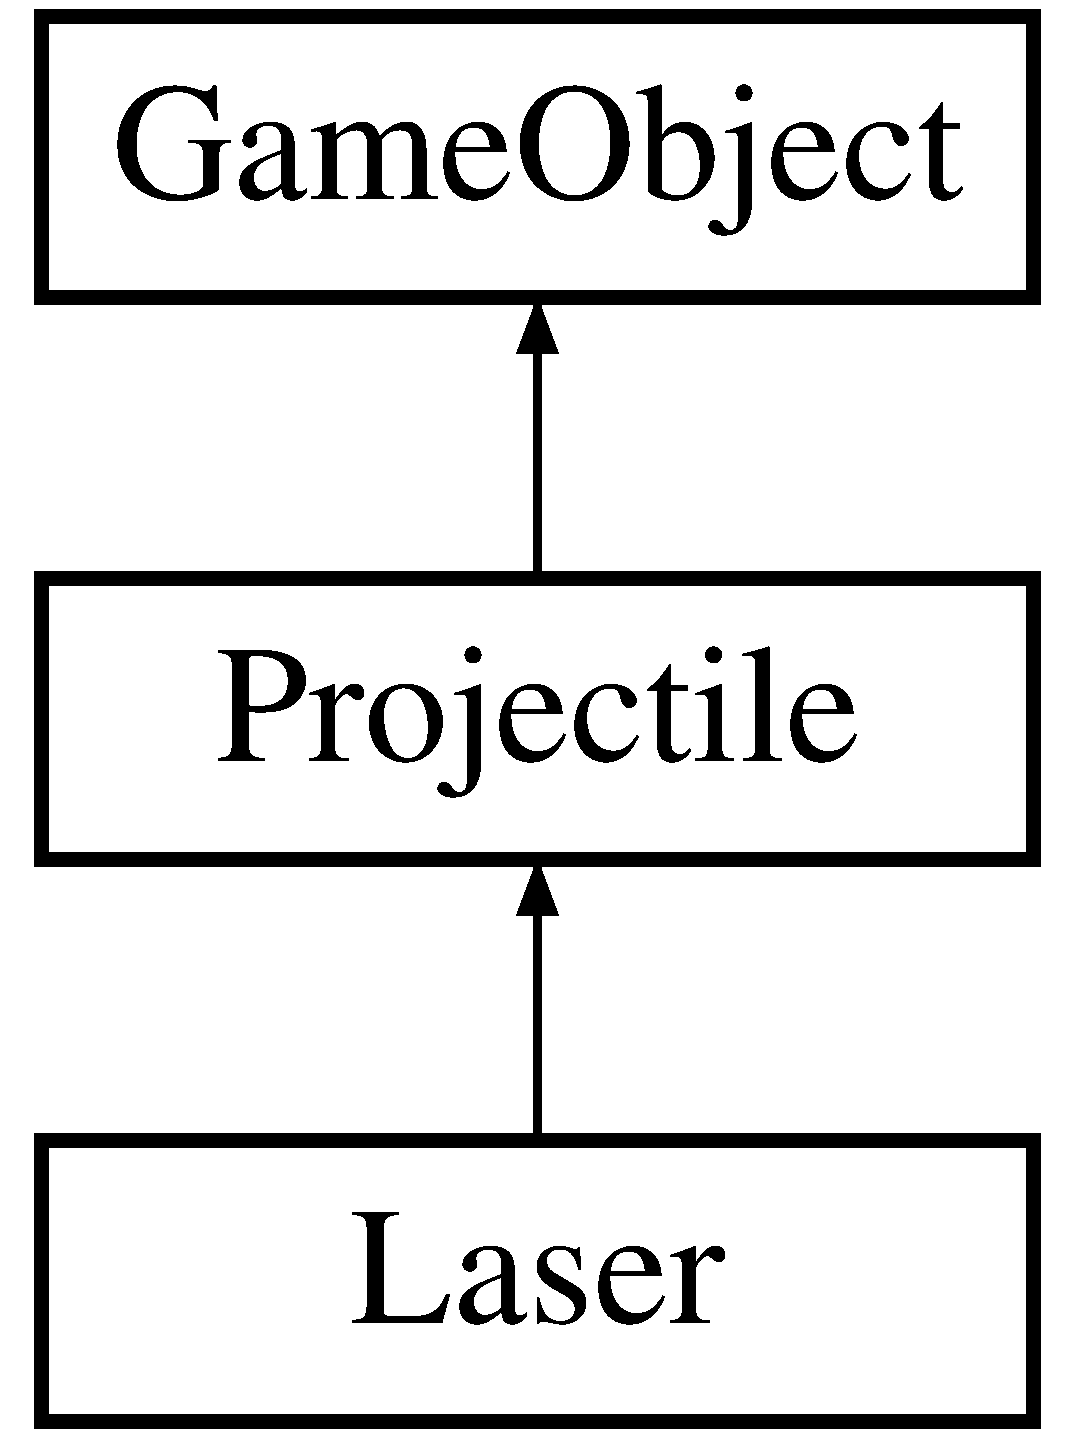
\includegraphics[height=3.000000cm]{class_laser}
\end{center}
\end{figure}
\subsection*{Public Member Functions}
\begin{DoxyCompactItemize}
\item 
\mbox{\hyperlink{class_laser_ac799230b67fc870ae9699efcf4ef27cb}{Laser}} (S\+D\+L\+\_\+\+Renderer $\ast$renderer, int x, int y)
\item 
\mbox{\hyperlink{class_laser_aa9baee5ed9775426e0b1d563c4687711}{$\sim$\+Laser}} ()
\item 
void \mbox{\hyperlink{class_laser_a1f2135281ecc1b318357633f4e7dd34c}{Logic}} ()
\end{DoxyCompactItemize}
\subsection*{Additional Inherited Members}


\subsection{Constructor \& Destructor Documentation}
\mbox{\Hypertarget{class_laser_ac799230b67fc870ae9699efcf4ef27cb}\label{class_laser_ac799230b67fc870ae9699efcf4ef27cb}} 
\index{Laser@{Laser}!Laser@{Laser}}
\index{Laser@{Laser}!Laser@{Laser}}
\subsubsection{\texorpdfstring{Laser()}{Laser()}}
{\footnotesize\ttfamily Laser\+::\+Laser (\begin{DoxyParamCaption}\item[{S\+D\+L\+\_\+\+Renderer $\ast$}]{renderer,  }\item[{int}]{x,  }\item[{int}]{y }\end{DoxyParamCaption})}

\mbox{\Hypertarget{class_laser_aa9baee5ed9775426e0b1d563c4687711}\label{class_laser_aa9baee5ed9775426e0b1d563c4687711}} 
\index{Laser@{Laser}!````~Laser@{$\sim$\+Laser}}
\index{````~Laser@{$\sim$\+Laser}!Laser@{Laser}}
\subsubsection{\texorpdfstring{$\sim$\+Laser()}{~Laser()}}
{\footnotesize\ttfamily Laser\+::$\sim$\+Laser (\begin{DoxyParamCaption}{ }\end{DoxyParamCaption})}



\subsection{Member Function Documentation}
\mbox{\Hypertarget{class_laser_a1f2135281ecc1b318357633f4e7dd34c}\label{class_laser_a1f2135281ecc1b318357633f4e7dd34c}} 
\index{Laser@{Laser}!Logic@{Logic}}
\index{Logic@{Logic}!Laser@{Laser}}
\subsubsection{\texorpdfstring{Logic()}{Logic()}}
{\footnotesize\ttfamily void Laser\+::\+Logic (\begin{DoxyParamCaption}{ }\end{DoxyParamCaption})\hspace{0.3cm}{\ttfamily [virtual]}}



Reimplemented from \mbox{\hyperlink{class_game_object_a79510ffc77339fe850491dce9f580fa9}{Game\+Object}}.



The documentation for this class was generated from the following files\+:\begin{DoxyCompactItemize}
\item 
Eksamen\+Base/\+Game\+Objects/\mbox{\hyperlink{_laser_8h}{Laser.\+h}}\item 
Eksamen\+Base/\+Game\+Objects/\mbox{\hyperlink{_laser_8cpp}{Laser.\+cpp}}\end{DoxyCompactItemize}

\hypertarget{class_mystery_ship}{}\section{Mystery\+Ship Class Reference}
\label{class_mystery_ship}\index{Mystery\+Ship@{Mystery\+Ship}}


{\ttfamily \#include $<$Mystery\+Ship.\+h$>$}

Inheritance diagram for Mystery\+Ship\+:\begin{figure}[H]
\begin{center}
\leavevmode
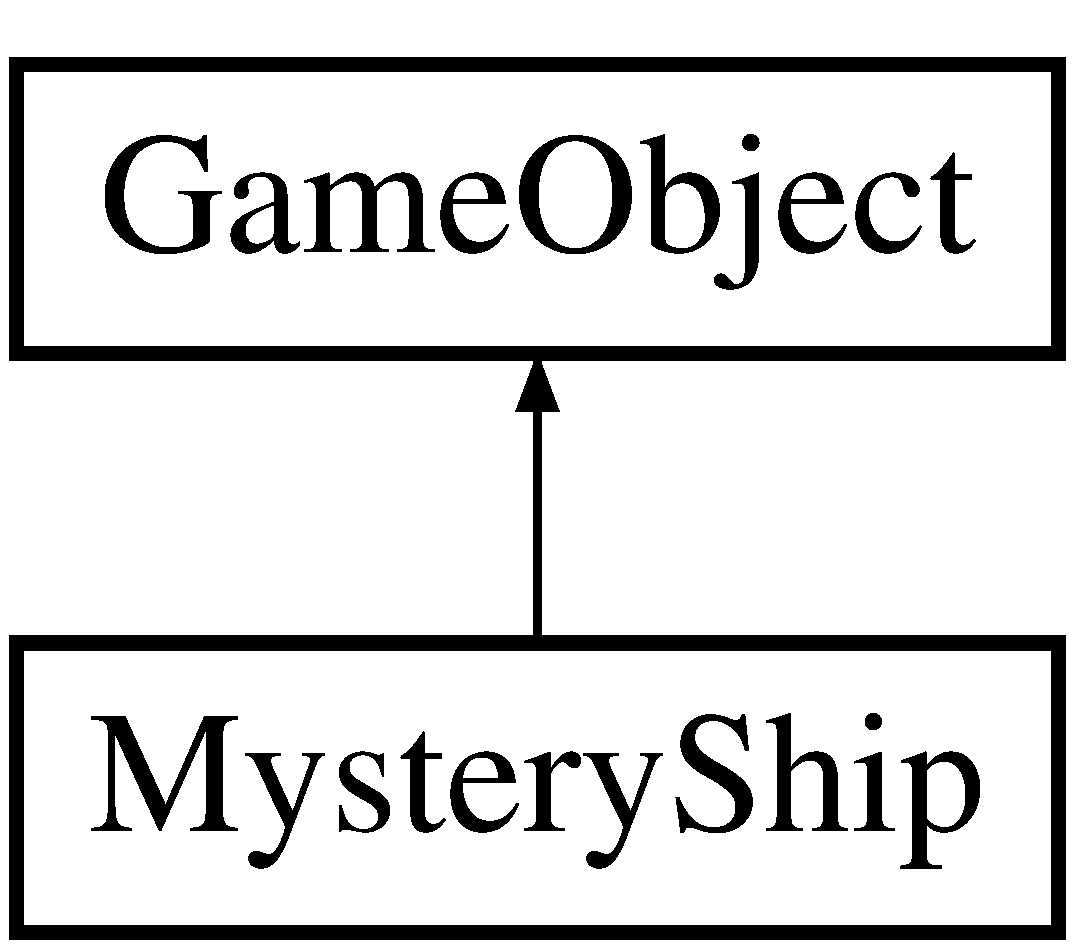
\includegraphics[height=2.000000cm]{class_mystery_ship}
\end{center}
\end{figure}
\subsection*{Public Member Functions}
\begin{DoxyCompactItemize}
\item 
\mbox{\hyperlink{class_mystery_ship_a0ba2e990784b0e4c1be1a4dc4a7c47c7}{Mystery\+Ship}} (S\+D\+L\+\_\+\+Renderer $\ast$renderer)
\item 
\mbox{\hyperlink{class_mystery_ship_a4396e9190999aa5b2879b4886d11814c}{$\sim$\+Mystery\+Ship}} ()
\item 
void \mbox{\hyperlink{class_mystery_ship_ace0406106086ab58d8da318e902ade0a}{Logic}} ()
\item 
void \mbox{\hyperlink{class_mystery_ship_ad79eee772a091f9ea2b194744450e5f2}{Input}} ()
\end{DoxyCompactItemize}
\subsection*{Additional Inherited Members}


\subsection{Constructor \& Destructor Documentation}
\mbox{\Hypertarget{class_mystery_ship_a0ba2e990784b0e4c1be1a4dc4a7c47c7}\label{class_mystery_ship_a0ba2e990784b0e4c1be1a4dc4a7c47c7}} 
\index{Mystery\+Ship@{Mystery\+Ship}!Mystery\+Ship@{Mystery\+Ship}}
\index{Mystery\+Ship@{Mystery\+Ship}!Mystery\+Ship@{Mystery\+Ship}}
\subsubsection{\texorpdfstring{Mystery\+Ship()}{MysteryShip()}}
{\footnotesize\ttfamily Mystery\+Ship\+::\+Mystery\+Ship (\begin{DoxyParamCaption}\item[{S\+D\+L\+\_\+\+Renderer $\ast$}]{renderer }\end{DoxyParamCaption})}

\mbox{\Hypertarget{class_mystery_ship_a4396e9190999aa5b2879b4886d11814c}\label{class_mystery_ship_a4396e9190999aa5b2879b4886d11814c}} 
\index{Mystery\+Ship@{Mystery\+Ship}!````~Mystery\+Ship@{$\sim$\+Mystery\+Ship}}
\index{````~Mystery\+Ship@{$\sim$\+Mystery\+Ship}!Mystery\+Ship@{Mystery\+Ship}}
\subsubsection{\texorpdfstring{$\sim$\+Mystery\+Ship()}{~MysteryShip()}}
{\footnotesize\ttfamily Mystery\+Ship\+::$\sim$\+Mystery\+Ship (\begin{DoxyParamCaption}{ }\end{DoxyParamCaption})}



\subsection{Member Function Documentation}
\mbox{\Hypertarget{class_mystery_ship_ad79eee772a091f9ea2b194744450e5f2}\label{class_mystery_ship_ad79eee772a091f9ea2b194744450e5f2}} 
\index{Mystery\+Ship@{Mystery\+Ship}!Input@{Input}}
\index{Input@{Input}!Mystery\+Ship@{Mystery\+Ship}}
\subsubsection{\texorpdfstring{Input()}{Input()}}
{\footnotesize\ttfamily void Mystery\+Ship\+::\+Input (\begin{DoxyParamCaption}{ }\end{DoxyParamCaption})\hspace{0.3cm}{\ttfamily [virtual]}}



Reimplemented from \mbox{\hyperlink{class_game_object_a430742cf91abb99337c556c88bef880a}{Game\+Object}}.

\mbox{\Hypertarget{class_mystery_ship_ace0406106086ab58d8da318e902ade0a}\label{class_mystery_ship_ace0406106086ab58d8da318e902ade0a}} 
\index{Mystery\+Ship@{Mystery\+Ship}!Logic@{Logic}}
\index{Logic@{Logic}!Mystery\+Ship@{Mystery\+Ship}}
\subsubsection{\texorpdfstring{Logic()}{Logic()}}
{\footnotesize\ttfamily void Mystery\+Ship\+::\+Logic (\begin{DoxyParamCaption}{ }\end{DoxyParamCaption})\hspace{0.3cm}{\ttfamily [virtual]}}



Reimplemented from \mbox{\hyperlink{class_game_object_a79510ffc77339fe850491dce9f580fa9}{Game\+Object}}.



The documentation for this class was generated from the following files\+:\begin{DoxyCompactItemize}
\item 
Eksamen\+Base/\+Game\+Objects/\mbox{\hyperlink{_mystery_ship_8h}{Mystery\+Ship.\+h}}\item 
Eksamen\+Base/\+Game\+Objects/\mbox{\hyperlink{_mystery_ship_8cpp}{Mystery\+Ship.\+cpp}}\end{DoxyCompactItemize}

\hypertarget{class_objects_pool}{}\section{Objects\+Pool Class Reference}
\label{class_objects_pool}\index{Objects\+Pool@{Objects\+Pool}}


{\ttfamily \#include $<$Objects\+Pool.\+h$>$}

\subsection*{Public Member Functions}
\begin{DoxyCompactItemize}
\item 
\mbox{\hyperlink{class_objects_pool_a0895698090f1d06cefc290b51bcd6197}{$\sim$\+Objects\+Pool}} ()
\item 
std\+::shared\+\_\+ptr$<$ \mbox{\hyperlink{class_game_object}{Game\+Object}} $>$ \mbox{\hyperlink{class_objects_pool_a0cb6ec80efacce659b008ab8bc000aa9}{Get\+Enemy\+Attack}} (S\+D\+L\+\_\+\+Renderer $\ast$renderer, int x, int y)
\item 
std\+::shared\+\_\+ptr$<$ \mbox{\hyperlink{class_game_object}{Game\+Object}} $>$ \mbox{\hyperlink{class_objects_pool_a97601dd9984711e20f2f9984a51a1741}{Get\+Snake}} (S\+D\+L\+\_\+\+Renderer $\ast$renderer, int x, int y)
\end{DoxyCompactItemize}
\subsection*{Static Public Member Functions}
\begin{DoxyCompactItemize}
\item 
static \mbox{\hyperlink{class_objects_pool}{Objects\+Pool}} \& \mbox{\hyperlink{class_objects_pool_aca7dadcb65812523bc0f910cf8183884}{get\+Instance}} ()
\end{DoxyCompactItemize}


\subsection{Constructor \& Destructor Documentation}
\mbox{\Hypertarget{class_objects_pool_a0895698090f1d06cefc290b51bcd6197}\label{class_objects_pool_a0895698090f1d06cefc290b51bcd6197}} 
\index{Objects\+Pool@{Objects\+Pool}!````~Objects\+Pool@{$\sim$\+Objects\+Pool}}
\index{````~Objects\+Pool@{$\sim$\+Objects\+Pool}!Objects\+Pool@{Objects\+Pool}}
\subsubsection{\texorpdfstring{$\sim$\+Objects\+Pool()}{~ObjectsPool()}}
{\footnotesize\ttfamily Objects\+Pool\+::$\sim$\+Objects\+Pool (\begin{DoxyParamCaption}{ }\end{DoxyParamCaption})}



\subsection{Member Function Documentation}
\mbox{\Hypertarget{class_objects_pool_a0cb6ec80efacce659b008ab8bc000aa9}\label{class_objects_pool_a0cb6ec80efacce659b008ab8bc000aa9}} 
\index{Objects\+Pool@{Objects\+Pool}!Get\+Enemy\+Attack@{Get\+Enemy\+Attack}}
\index{Get\+Enemy\+Attack@{Get\+Enemy\+Attack}!Objects\+Pool@{Objects\+Pool}}
\subsubsection{\texorpdfstring{Get\+Enemy\+Attack()}{GetEnemyAttack()}}
{\footnotesize\ttfamily std\+::shared\+\_\+ptr$<$ \mbox{\hyperlink{class_game_object}{Game\+Object}} $>$ Objects\+Pool\+::\+Get\+Enemy\+Attack (\begin{DoxyParamCaption}\item[{S\+D\+L\+\_\+\+Renderer $\ast$}]{renderer,  }\item[{int}]{x,  }\item[{int}]{y }\end{DoxyParamCaption})}

\mbox{\Hypertarget{class_objects_pool_aca7dadcb65812523bc0f910cf8183884}\label{class_objects_pool_aca7dadcb65812523bc0f910cf8183884}} 
\index{Objects\+Pool@{Objects\+Pool}!get\+Instance@{get\+Instance}}
\index{get\+Instance@{get\+Instance}!Objects\+Pool@{Objects\+Pool}}
\subsubsection{\texorpdfstring{get\+Instance()}{getInstance()}}
{\footnotesize\ttfamily static \mbox{\hyperlink{class_objects_pool}{Objects\+Pool}}\& Objects\+Pool\+::get\+Instance (\begin{DoxyParamCaption}{ }\end{DoxyParamCaption})\hspace{0.3cm}{\ttfamily [inline]}, {\ttfamily [static]}}

\mbox{\Hypertarget{class_objects_pool_a97601dd9984711e20f2f9984a51a1741}\label{class_objects_pool_a97601dd9984711e20f2f9984a51a1741}} 
\index{Objects\+Pool@{Objects\+Pool}!Get\+Snake@{Get\+Snake}}
\index{Get\+Snake@{Get\+Snake}!Objects\+Pool@{Objects\+Pool}}
\subsubsection{\texorpdfstring{Get\+Snake()}{GetSnake()}}
{\footnotesize\ttfamily std\+::shared\+\_\+ptr$<$ \mbox{\hyperlink{class_game_object}{Game\+Object}} $>$ Objects\+Pool\+::\+Get\+Snake (\begin{DoxyParamCaption}\item[{S\+D\+L\+\_\+\+Renderer $\ast$}]{renderer,  }\item[{int}]{x,  }\item[{int}]{y }\end{DoxyParamCaption})}



The documentation for this class was generated from the following files\+:\begin{DoxyCompactItemize}
\item 
Eksamen\+Base/\+Handlers/\mbox{\hyperlink{_objects_pool_8h}{Objects\+Pool.\+h}}\item 
Eksamen\+Base/\+Handlers/\mbox{\hyperlink{_objects_pool_8cpp}{Objects\+Pool.\+cpp}}\end{DoxyCompactItemize}

\hypertarget{class_player}{}\section{Player Class Reference}
\label{class_player}\index{Player@{Player}}


{\ttfamily \#include $<$Player.\+h$>$}

Inheritance diagram for Player\+:\begin{figure}[H]
\begin{center}
\leavevmode
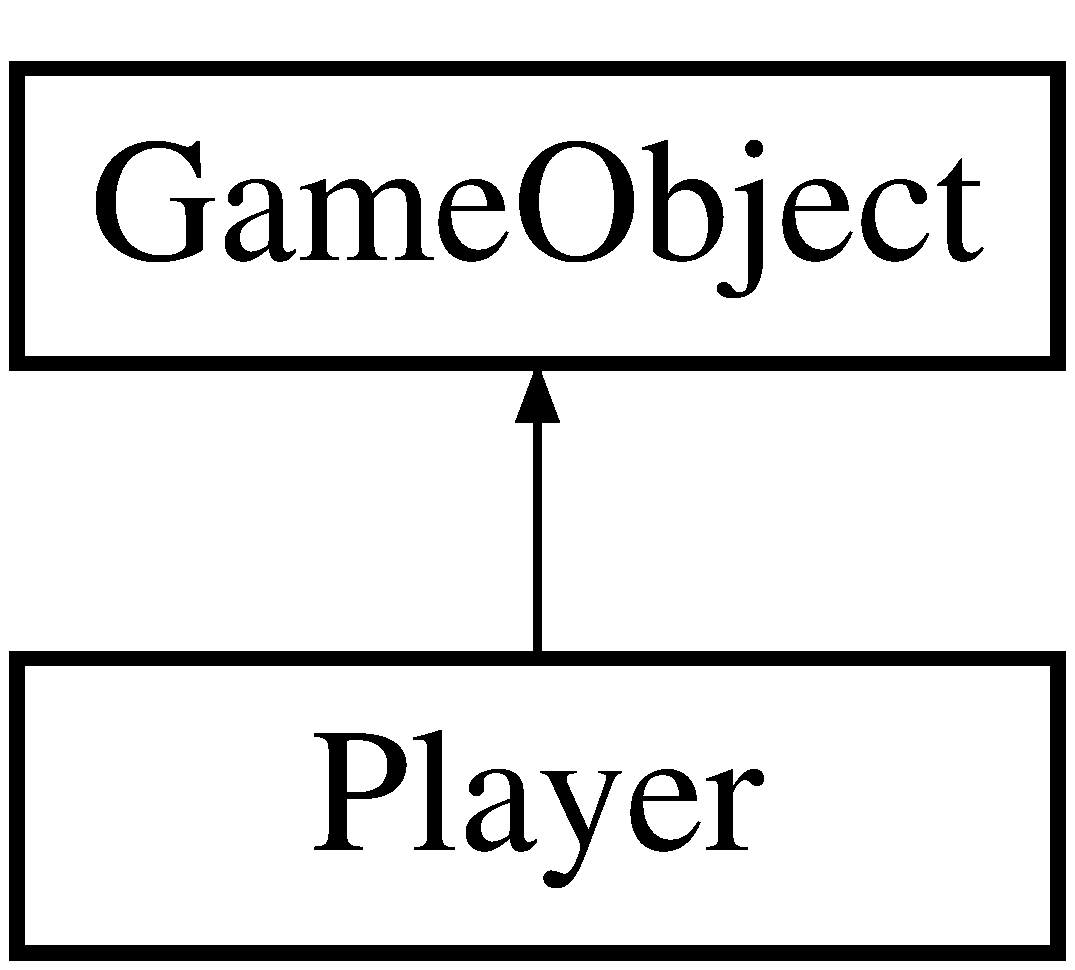
\includegraphics[height=2.000000cm]{class_player}
\end{center}
\end{figure}
\subsection*{Public Member Functions}
\begin{DoxyCompactItemize}
\item 
\mbox{\hyperlink{class_player_a753df4f66aa114c0789ba730199e4a01}{Player}} (S\+D\+L\+\_\+\+Renderer $\ast$renderer, int x, int y)
\item 
\mbox{\hyperlink{class_player_a749d2c00e1fe0f5c2746f7505a58c062}{$\sim$\+Player}} ()
\item 
void \mbox{\hyperlink{class_player_ae30c8d49de94ee8c73ed6ab6315a2854}{Logic}} ()
\item 
void \mbox{\hyperlink{class_player_a65a76094cff6f149d5847d2110fe443d}{Input}} ()
\item 
void \mbox{\hyperlink{class_player_a7da8c52d956abfc5a31742545c5d50b8}{Replenish}} ()
\begin{DoxyCompactList}\small\item\em Sets the bool m\+\_\+replenished to true \end{DoxyCompactList}\end{DoxyCompactItemize}
\subsection*{Additional Inherited Members}


\subsection{Constructor \& Destructor Documentation}
\mbox{\Hypertarget{class_player_a753df4f66aa114c0789ba730199e4a01}\label{class_player_a753df4f66aa114c0789ba730199e4a01}} 
\index{Player@{Player}!Player@{Player}}
\index{Player@{Player}!Player@{Player}}
\subsubsection{\texorpdfstring{Player()}{Player()}}
{\footnotesize\ttfamily Player\+::\+Player (\begin{DoxyParamCaption}\item[{S\+D\+L\+\_\+\+Renderer $\ast$}]{renderer,  }\item[{int}]{x,  }\item[{int}]{y }\end{DoxyParamCaption})}

\mbox{\Hypertarget{class_player_a749d2c00e1fe0f5c2746f7505a58c062}\label{class_player_a749d2c00e1fe0f5c2746f7505a58c062}} 
\index{Player@{Player}!````~Player@{$\sim$\+Player}}
\index{````~Player@{$\sim$\+Player}!Player@{Player}}
\subsubsection{\texorpdfstring{$\sim$\+Player()}{~Player()}}
{\footnotesize\ttfamily Player\+::$\sim$\+Player (\begin{DoxyParamCaption}{ }\end{DoxyParamCaption})}



\subsection{Member Function Documentation}
\mbox{\Hypertarget{class_player_a65a76094cff6f149d5847d2110fe443d}\label{class_player_a65a76094cff6f149d5847d2110fe443d}} 
\index{Player@{Player}!Input@{Input}}
\index{Input@{Input}!Player@{Player}}
\subsubsection{\texorpdfstring{Input()}{Input()}}
{\footnotesize\ttfamily void Player\+::\+Input (\begin{DoxyParamCaption}{ }\end{DoxyParamCaption})\hspace{0.3cm}{\ttfamily [virtual]}}



Reimplemented from \mbox{\hyperlink{class_game_object_a430742cf91abb99337c556c88bef880a}{Game\+Object}}.

\mbox{\Hypertarget{class_player_ae30c8d49de94ee8c73ed6ab6315a2854}\label{class_player_ae30c8d49de94ee8c73ed6ab6315a2854}} 
\index{Player@{Player}!Logic@{Logic}}
\index{Logic@{Logic}!Player@{Player}}
\subsubsection{\texorpdfstring{Logic()}{Logic()}}
{\footnotesize\ttfamily void Player\+::\+Logic (\begin{DoxyParamCaption}{ }\end{DoxyParamCaption})\hspace{0.3cm}{\ttfamily [virtual]}}



Reimplemented from \mbox{\hyperlink{class_game_object_a79510ffc77339fe850491dce9f580fa9}{Game\+Object}}.

\mbox{\Hypertarget{class_player_a7da8c52d956abfc5a31742545c5d50b8}\label{class_player_a7da8c52d956abfc5a31742545c5d50b8}} 
\index{Player@{Player}!Replenish@{Replenish}}
\index{Replenish@{Replenish}!Player@{Player}}
\subsubsection{\texorpdfstring{Replenish()}{Replenish()}}
{\footnotesize\ttfamily void Player\+::\+Replenish (\begin{DoxyParamCaption}{ }\end{DoxyParamCaption})}



Sets the bool m\+\_\+replenished to true 



The documentation for this class was generated from the following files\+:\begin{DoxyCompactItemize}
\item 
Eksamen\+Base/\+Game\+Objects/\mbox{\hyperlink{_player_8h}{Player.\+h}}\item 
Eksamen\+Base/\+Game\+Objects/\mbox{\hyperlink{_player_8cpp}{Player.\+cpp}}\end{DoxyCompactItemize}

\hypertarget{class_projectile}{}\section{Projectile Class Reference}
\label{class_projectile}\index{Projectile@{Projectile}}


{\ttfamily \#include $<$Projectile.\+h$>$}

Inheritance diagram for Projectile\+:\begin{figure}[H]
\begin{center}
\leavevmode
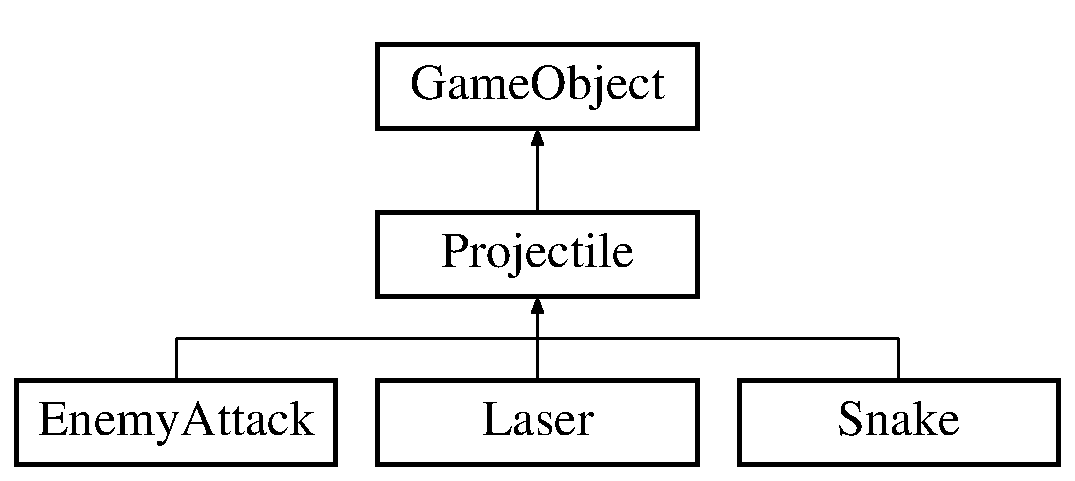
\includegraphics[height=3.000000cm]{class_projectile}
\end{center}
\end{figure}
\subsection*{Public Member Functions}
\begin{DoxyCompactItemize}
\item 
\mbox{\hyperlink{class_projectile_a0906140caebe54c0b087c7e6240f3084}{Projectile}} (S\+D\+L\+\_\+\+Renderer $\ast$renderer, int x, int y)
\item 
\mbox{\hyperlink{class_projectile_a94903e021fa2edab60ba3836ca0b937d}{$\sim$\+Projectile}} ()
\item 
void \mbox{\hyperlink{class_projectile_a871e265207d2bf2d5180152a7acf2d40}{Logic}} ()
\end{DoxyCompactItemize}
\subsection*{Protected Member Functions}
\begin{DoxyCompactItemize}
\item 
void \mbox{\hyperlink{class_projectile_a6baf0fc9681b7c13b64a1c82671e296f}{Check\+Position}} ()
\end{DoxyCompactItemize}
\subsection*{Protected Attributes}
\begin{DoxyCompactItemize}
\item 
\mbox{\hyperlink{class_game_object}{Game\+Object}} $\ast$ \mbox{\hyperlink{class_projectile_a1a76b3677c7be9a072e7097c34adc517}{owner}}
\item 
\mbox{\hyperlink{struct_game_object_1_1_vector2_d}{Vector2D}} \mbox{\hyperlink{class_projectile_a0e4b335bd16e41ec9f8b2f6b8006cac8}{direction}}
\end{DoxyCompactItemize}
\subsection*{Additional Inherited Members}


\subsection{Constructor \& Destructor Documentation}
\mbox{\Hypertarget{class_projectile_a0906140caebe54c0b087c7e6240f3084}\label{class_projectile_a0906140caebe54c0b087c7e6240f3084}} 
\index{Projectile@{Projectile}!Projectile@{Projectile}}
\index{Projectile@{Projectile}!Projectile@{Projectile}}
\subsubsection{\texorpdfstring{Projectile()}{Projectile()}}
{\footnotesize\ttfamily Projectile\+::\+Projectile (\begin{DoxyParamCaption}\item[{S\+D\+L\+\_\+\+Renderer $\ast$}]{renderer,  }\item[{int}]{x,  }\item[{int}]{y }\end{DoxyParamCaption})}

\mbox{\Hypertarget{class_projectile_a94903e021fa2edab60ba3836ca0b937d}\label{class_projectile_a94903e021fa2edab60ba3836ca0b937d}} 
\index{Projectile@{Projectile}!````~Projectile@{$\sim$\+Projectile}}
\index{````~Projectile@{$\sim$\+Projectile}!Projectile@{Projectile}}
\subsubsection{\texorpdfstring{$\sim$\+Projectile()}{~Projectile()}}
{\footnotesize\ttfamily Projectile\+::$\sim$\+Projectile (\begin{DoxyParamCaption}{ }\end{DoxyParamCaption})}



\subsection{Member Function Documentation}
\mbox{\Hypertarget{class_projectile_a6baf0fc9681b7c13b64a1c82671e296f}\label{class_projectile_a6baf0fc9681b7c13b64a1c82671e296f}} 
\index{Projectile@{Projectile}!Check\+Position@{Check\+Position}}
\index{Check\+Position@{Check\+Position}!Projectile@{Projectile}}
\subsubsection{\texorpdfstring{Check\+Position()}{CheckPosition()}}
{\footnotesize\ttfamily void Projectile\+::\+Check\+Position (\begin{DoxyParamCaption}{ }\end{DoxyParamCaption})\hspace{0.3cm}{\ttfamily [protected]}}

\mbox{\Hypertarget{class_projectile_a871e265207d2bf2d5180152a7acf2d40}\label{class_projectile_a871e265207d2bf2d5180152a7acf2d40}} 
\index{Projectile@{Projectile}!Logic@{Logic}}
\index{Logic@{Logic}!Projectile@{Projectile}}
\subsubsection{\texorpdfstring{Logic()}{Logic()}}
{\footnotesize\ttfamily void Projectile\+::\+Logic (\begin{DoxyParamCaption}{ }\end{DoxyParamCaption})\hspace{0.3cm}{\ttfamily [virtual]}}



Reimplemented from \mbox{\hyperlink{class_game_object_a79510ffc77339fe850491dce9f580fa9}{Game\+Object}}.



Reimplemented in \mbox{\hyperlink{class_snake_a1f01e21a73734f9c0d701ec02a9d2e41}{Snake}}.



\subsection{Member Data Documentation}
\mbox{\Hypertarget{class_projectile_a0e4b335bd16e41ec9f8b2f6b8006cac8}\label{class_projectile_a0e4b335bd16e41ec9f8b2f6b8006cac8}} 
\index{Projectile@{Projectile}!direction@{direction}}
\index{direction@{direction}!Projectile@{Projectile}}
\subsubsection{\texorpdfstring{direction}{direction}}
{\footnotesize\ttfamily \mbox{\hyperlink{struct_game_object_1_1_vector2_d}{Vector2D}} Projectile\+::direction\hspace{0.3cm}{\ttfamily [protected]}}

\mbox{\Hypertarget{class_projectile_a1a76b3677c7be9a072e7097c34adc517}\label{class_projectile_a1a76b3677c7be9a072e7097c34adc517}} 
\index{Projectile@{Projectile}!owner@{owner}}
\index{owner@{owner}!Projectile@{Projectile}}
\subsubsection{\texorpdfstring{owner}{owner}}
{\footnotesize\ttfamily \mbox{\hyperlink{class_game_object}{Game\+Object}}$\ast$ Projectile\+::owner\hspace{0.3cm}{\ttfamily [protected]}}



The documentation for this class was generated from the following files\+:\begin{DoxyCompactItemize}
\item 
Eksamen\+Base/\+Game\+Objects/\mbox{\hyperlink{_projectile_8h}{Projectile.\+h}}\item 
Eksamen\+Base/\+Game\+Objects/\mbox{\hyperlink{_projectile_8cpp}{Projectile.\+cpp}}\end{DoxyCompactItemize}

\hypertarget{class_snake}{}\section{Snake Class Reference}
\label{class_snake}\index{Snake@{Snake}}


{\ttfamily \#include $<$Snake.\+h$>$}

Inheritance diagram for Snake\+:\begin{figure}[H]
\begin{center}
\leavevmode
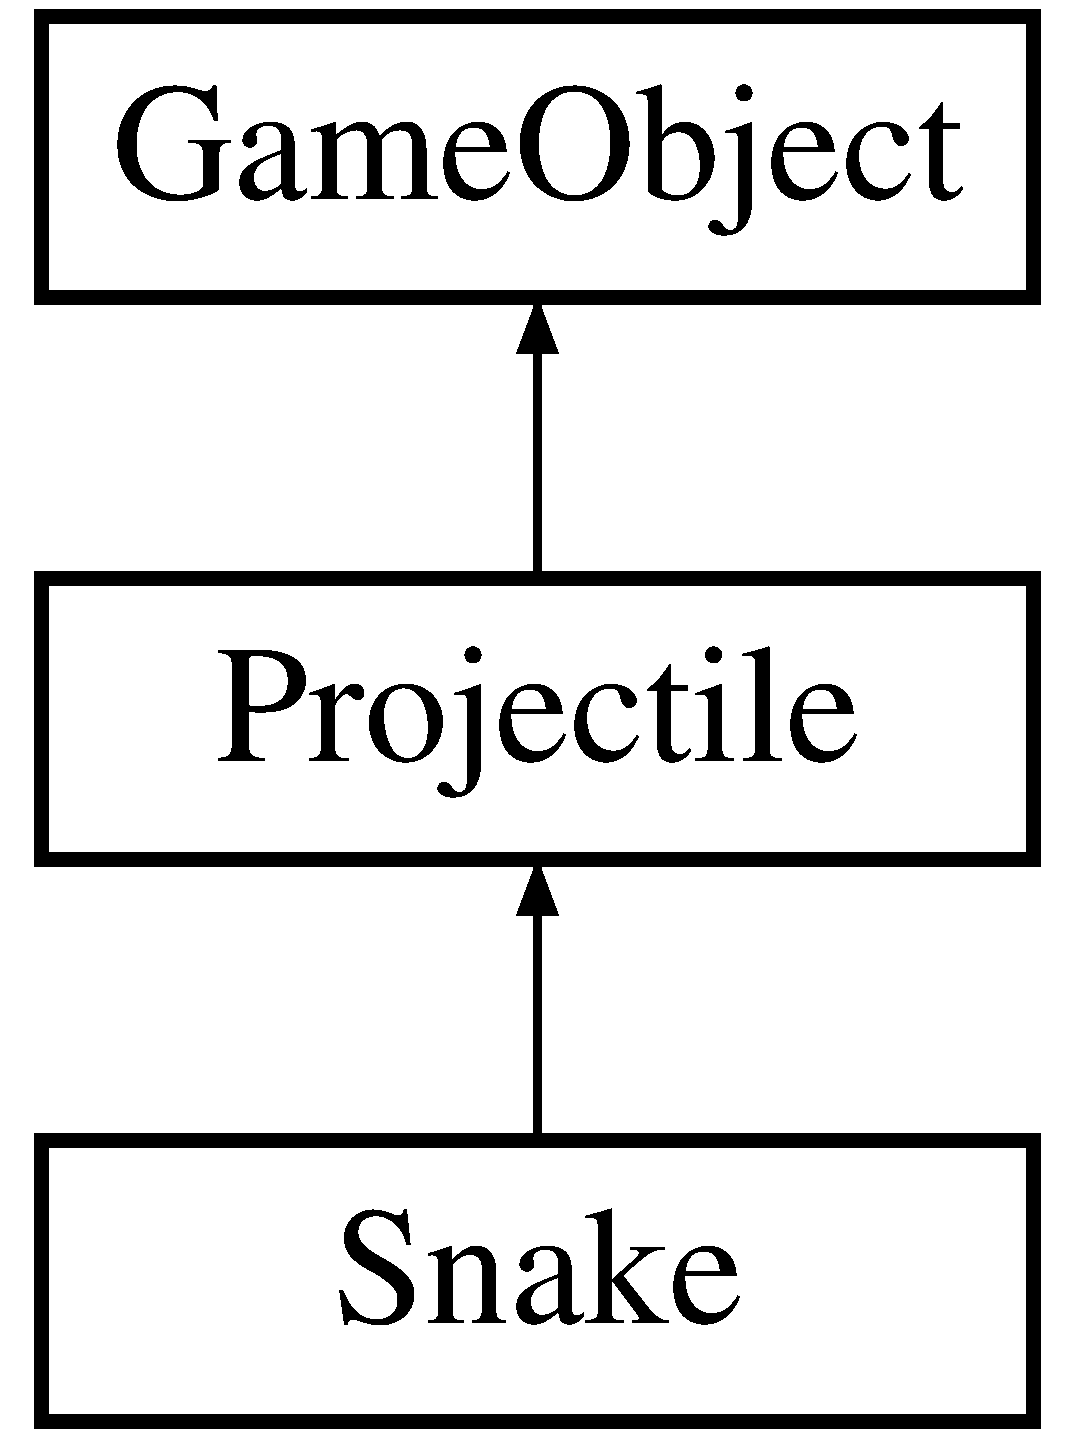
\includegraphics[height=3.000000cm]{class_snake}
\end{center}
\end{figure}
\subsection*{Public Member Functions}
\begin{DoxyCompactItemize}
\item 
\mbox{\hyperlink{class_snake_ae54c34f487c04c54bd7daadbe42d3a4b}{Snake}} (S\+D\+L\+\_\+\+Renderer $\ast$renderer, int x, int y)
\item 
\mbox{\hyperlink{class_snake_a941fbaad96ee33ca3a7c30c28ca44ef8}{$\sim$\+Snake}} ()
\item 
void \mbox{\hyperlink{class_snake_a1f01e21a73734f9c0d701ec02a9d2e41}{Logic}} ()
\end{DoxyCompactItemize}
\subsection*{Additional Inherited Members}


\subsection{Constructor \& Destructor Documentation}
\mbox{\Hypertarget{class_snake_ae54c34f487c04c54bd7daadbe42d3a4b}\label{class_snake_ae54c34f487c04c54bd7daadbe42d3a4b}} 
\index{Snake@{Snake}!Snake@{Snake}}
\index{Snake@{Snake}!Snake@{Snake}}
\subsubsection{\texorpdfstring{Snake()}{Snake()}}
{\footnotesize\ttfamily Snake\+::\+Snake (\begin{DoxyParamCaption}\item[{S\+D\+L\+\_\+\+Renderer $\ast$}]{renderer,  }\item[{int}]{x,  }\item[{int}]{y }\end{DoxyParamCaption})}

\mbox{\Hypertarget{class_snake_a941fbaad96ee33ca3a7c30c28ca44ef8}\label{class_snake_a941fbaad96ee33ca3a7c30c28ca44ef8}} 
\index{Snake@{Snake}!````~Snake@{$\sim$\+Snake}}
\index{````~Snake@{$\sim$\+Snake}!Snake@{Snake}}
\subsubsection{\texorpdfstring{$\sim$\+Snake()}{~Snake()}}
{\footnotesize\ttfamily Snake\+::$\sim$\+Snake (\begin{DoxyParamCaption}{ }\end{DoxyParamCaption})}



\subsection{Member Function Documentation}
\mbox{\Hypertarget{class_snake_a1f01e21a73734f9c0d701ec02a9d2e41}\label{class_snake_a1f01e21a73734f9c0d701ec02a9d2e41}} 
\index{Snake@{Snake}!Logic@{Logic}}
\index{Logic@{Logic}!Snake@{Snake}}
\subsubsection{\texorpdfstring{Logic()}{Logic()}}
{\footnotesize\ttfamily void Snake\+::\+Logic (\begin{DoxyParamCaption}{ }\end{DoxyParamCaption})\hspace{0.3cm}{\ttfamily [virtual]}}



Reimplemented from \mbox{\hyperlink{class_projectile_a871e265207d2bf2d5180152a7acf2d40}{Projectile}}.



The documentation for this class was generated from the following files\+:\begin{DoxyCompactItemize}
\item 
Eksamen\+Base/\+Game\+Objects/\mbox{\hyperlink{_snake_8h}{Snake.\+h}}\item 
Eksamen\+Base/\+Game\+Objects/\mbox{\hyperlink{_snake_8cpp}{Snake.\+cpp}}\end{DoxyCompactItemize}

\hypertarget{class_sound_manager}{}\section{Sound\+Manager Class Reference}
\label{class_sound_manager}\index{Sound\+Manager@{Sound\+Manager}}


{\ttfamily \#include $<$Sound\+Manager.\+h$>$}

\subsection*{Public Member Functions}
\begin{DoxyCompactItemize}
\item 
\mbox{\hyperlink{class_sound_manager_ad5dbf8eab22db48ff8f3db51b02f8938}{$\sim$\+Sound\+Manager}} ()
\item 
bool \mbox{\hyperlink{class_sound_manager_af1ee5e29fca894a8ac9aeeb56b81f21d}{Init}} ()
\begin{DoxyCompactList}\small\item\em Inits the soundmanager \end{DoxyCompactList}\item 
void \mbox{\hyperlink{class_sound_manager_af84f2acbde4d8c0d8f5b47c2d917e486}{Play\+Sound}} (std\+::string sound\+Name)
\begin{DoxyCompactList}\small\item\em Plays a sound with the given name \end{DoxyCompactList}\item 
void \mbox{\hyperlink{class_sound_manager_ab4f6bc3b9c203232424b10da9912cf1b}{Play\+Music}} ()
\begin{DoxyCompactList}\small\item\em Starts the game music \end{DoxyCompactList}\item 
void \mbox{\hyperlink{class_sound_manager_a8b26fc4974bebd09b4bd7e108e8394ae}{Stop\+Music}} ()
\begin{DoxyCompactList}\small\item\em Stops the game music \end{DoxyCompactList}\item 
bool \mbox{\hyperlink{class_sound_manager_ae41fb3a3efb5b1fc9b39bd2764a032cc}{Music\+Playing}} ()
\begin{DoxyCompactList}\small\item\em Returns true if music is playing \end{DoxyCompactList}\end{DoxyCompactItemize}
\subsection*{Static Public Member Functions}
\begin{DoxyCompactItemize}
\item 
static \mbox{\hyperlink{class_sound_manager}{Sound\+Manager}} \& \mbox{\hyperlink{class_sound_manager_a4f8f0b2d539d055f4c1de8c47d483cb3}{get\+Instance}} ()
\end{DoxyCompactItemize}


\subsection{Constructor \& Destructor Documentation}
\mbox{\Hypertarget{class_sound_manager_ad5dbf8eab22db48ff8f3db51b02f8938}\label{class_sound_manager_ad5dbf8eab22db48ff8f3db51b02f8938}} 
\index{Sound\+Manager@{Sound\+Manager}!````~Sound\+Manager@{$\sim$\+Sound\+Manager}}
\index{````~Sound\+Manager@{$\sim$\+Sound\+Manager}!Sound\+Manager@{Sound\+Manager}}
\subsubsection{\texorpdfstring{$\sim$\+Sound\+Manager()}{~SoundManager()}}
{\footnotesize\ttfamily Sound\+Manager\+::$\sim$\+Sound\+Manager (\begin{DoxyParamCaption}{ }\end{DoxyParamCaption})}



\subsection{Member Function Documentation}
\mbox{\Hypertarget{class_sound_manager_a4f8f0b2d539d055f4c1de8c47d483cb3}\label{class_sound_manager_a4f8f0b2d539d055f4c1de8c47d483cb3}} 
\index{Sound\+Manager@{Sound\+Manager}!get\+Instance@{get\+Instance}}
\index{get\+Instance@{get\+Instance}!Sound\+Manager@{Sound\+Manager}}
\subsubsection{\texorpdfstring{get\+Instance()}{getInstance()}}
{\footnotesize\ttfamily static \mbox{\hyperlink{class_sound_manager}{Sound\+Manager}}\& Sound\+Manager\+::get\+Instance (\begin{DoxyParamCaption}{ }\end{DoxyParamCaption})\hspace{0.3cm}{\ttfamily [inline]}, {\ttfamily [static]}}

\mbox{\Hypertarget{class_sound_manager_af1ee5e29fca894a8ac9aeeb56b81f21d}\label{class_sound_manager_af1ee5e29fca894a8ac9aeeb56b81f21d}} 
\index{Sound\+Manager@{Sound\+Manager}!Init@{Init}}
\index{Init@{Init}!Sound\+Manager@{Sound\+Manager}}
\subsubsection{\texorpdfstring{Init()}{Init()}}
{\footnotesize\ttfamily bool Sound\+Manager\+::\+Init (\begin{DoxyParamCaption}{ }\end{DoxyParamCaption})}



Inits the soundmanager 

\mbox{\Hypertarget{class_sound_manager_ae41fb3a3efb5b1fc9b39bd2764a032cc}\label{class_sound_manager_ae41fb3a3efb5b1fc9b39bd2764a032cc}} 
\index{Sound\+Manager@{Sound\+Manager}!Music\+Playing@{Music\+Playing}}
\index{Music\+Playing@{Music\+Playing}!Sound\+Manager@{Sound\+Manager}}
\subsubsection{\texorpdfstring{Music\+Playing()}{MusicPlaying()}}
{\footnotesize\ttfamily bool Sound\+Manager\+::\+Music\+Playing (\begin{DoxyParamCaption}{ }\end{DoxyParamCaption})}



Returns true if music is playing 

\begin{DoxyReturn}{Returns}

\end{DoxyReturn}
\mbox{\Hypertarget{class_sound_manager_ab4f6bc3b9c203232424b10da9912cf1b}\label{class_sound_manager_ab4f6bc3b9c203232424b10da9912cf1b}} 
\index{Sound\+Manager@{Sound\+Manager}!Play\+Music@{Play\+Music}}
\index{Play\+Music@{Play\+Music}!Sound\+Manager@{Sound\+Manager}}
\subsubsection{\texorpdfstring{Play\+Music()}{PlayMusic()}}
{\footnotesize\ttfamily void Sound\+Manager\+::\+Play\+Music (\begin{DoxyParamCaption}{ }\end{DoxyParamCaption})}



Starts the game music 

\mbox{\Hypertarget{class_sound_manager_af84f2acbde4d8c0d8f5b47c2d917e486}\label{class_sound_manager_af84f2acbde4d8c0d8f5b47c2d917e486}} 
\index{Sound\+Manager@{Sound\+Manager}!Play\+Sound@{Play\+Sound}}
\index{Play\+Sound@{Play\+Sound}!Sound\+Manager@{Sound\+Manager}}
\subsubsection{\texorpdfstring{Play\+Sound()}{PlaySound()}}
{\footnotesize\ttfamily void Sound\+Manager\+::\+Play\+Sound (\begin{DoxyParamCaption}\item[{std\+::string}]{sound\+Name }\end{DoxyParamCaption})}



Plays a sound with the given name 


\begin{DoxyParams}{Parameters}
{\em sound\+Name} & \\
\hline
\end{DoxyParams}
\mbox{\Hypertarget{class_sound_manager_a8b26fc4974bebd09b4bd7e108e8394ae}\label{class_sound_manager_a8b26fc4974bebd09b4bd7e108e8394ae}} 
\index{Sound\+Manager@{Sound\+Manager}!Stop\+Music@{Stop\+Music}}
\index{Stop\+Music@{Stop\+Music}!Sound\+Manager@{Sound\+Manager}}
\subsubsection{\texorpdfstring{Stop\+Music()}{StopMusic()}}
{\footnotesize\ttfamily void Sound\+Manager\+::\+Stop\+Music (\begin{DoxyParamCaption}{ }\end{DoxyParamCaption})}



Stops the game music 



The documentation for this class was generated from the following files\+:\begin{DoxyCompactItemize}
\item 
Eksamen\+Base/\+Handlers/\mbox{\hyperlink{_sound_manager_8h}{Sound\+Manager.\+h}}\item 
Eksamen\+Base/\+Handlers/\mbox{\hyperlink{_sound_manager_8cpp}{Sound\+Manager.\+cpp}}\end{DoxyCompactItemize}

\hypertarget{class_text}{}\section{Text Class Reference}
\label{class_text}\index{Text@{Text}}


{\ttfamily \#include $<$Text.\+h$>$}

\subsection*{Public Member Functions}
\begin{DoxyCompactItemize}
\item 
\mbox{\hyperlink{class_text_a1a244ff955d98640e0046acef0659413}{Text}} (S\+D\+L\+\_\+\+Renderer $\ast$renderer, std\+::string text, S\+D\+L\+\_\+\+Color color, int size, int x, int y, int w, int h)
\item 
\mbox{\hyperlink{class_text_a2d49e5c280e205125b149f7777ae30c7}{$\sim$\+Text}} ()
\item 
void \mbox{\hyperlink{class_text_ab2d8c95b3d746ae3e8c0fba8318743c9}{set\+Text}} (std\+::string text)
\begin{DoxyCompactList}\small\item\em Changes the text \end{DoxyCompactList}\item 
void \mbox{\hyperlink{class_text_abb8e725b17de08304a97119d39df5cc1}{set\+Color}} (S\+D\+L\+\_\+\+Color color)
\begin{DoxyCompactList}\small\item\em Changes the color of the text \end{DoxyCompactList}\item 
void \mbox{\hyperlink{class_text_a55995c22d9a3166ccd856f3b632f2354}{set\+Position}} (int x, int y)
\begin{DoxyCompactList}\small\item\em Changes the position of the text \end{DoxyCompactList}\item 
void \mbox{\hyperlink{class_text_a654ac74524e48652f9aa789d2612052b}{set\+Visible}} (bool visible)
\begin{DoxyCompactList}\small\item\em If text should be visible or not \end{DoxyCompactList}\item 
void \mbox{\hyperlink{class_text_aa3075bc13723baa1a72bdd2a2a1ba509}{set\+Blink}} (bool should\+Blink)
\begin{DoxyCompactList}\small\item\em Turn blinking on and off \end{DoxyCompactList}\item 
void \mbox{\hyperlink{class_text_af4bb084ff0f66ad827ef6b006f9b0ebd}{Draw}} ()
\begin{DoxyCompactList}\small\item\em Draws the text onto the screen \end{DoxyCompactList}\end{DoxyCompactItemize}
\subsection*{Public Attributes}
\begin{DoxyCompactItemize}
\item 
S\+D\+L\+\_\+\+Texture $\ast$ \mbox{\hyperlink{class_text_a0db81807f575e9f4ff86bdae450ee246}{text\+Texture}}
\end{DoxyCompactItemize}


\subsection{Constructor \& Destructor Documentation}
\mbox{\Hypertarget{class_text_a1a244ff955d98640e0046acef0659413}\label{class_text_a1a244ff955d98640e0046acef0659413}} 
\index{Text@{Text}!Text@{Text}}
\index{Text@{Text}!Text@{Text}}
\subsubsection{\texorpdfstring{Text()}{Text()}}
{\footnotesize\ttfamily Text\+::\+Text (\begin{DoxyParamCaption}\item[{S\+D\+L\+\_\+\+Renderer $\ast$}]{renderer,  }\item[{std\+::string}]{text,  }\item[{S\+D\+L\+\_\+\+Color}]{color,  }\item[{int}]{size,  }\item[{int}]{x,  }\item[{int}]{y,  }\item[{int}]{w,  }\item[{int}]{h }\end{DoxyParamCaption})}

\mbox{\Hypertarget{class_text_a2d49e5c280e205125b149f7777ae30c7}\label{class_text_a2d49e5c280e205125b149f7777ae30c7}} 
\index{Text@{Text}!````~Text@{$\sim$\+Text}}
\index{````~Text@{$\sim$\+Text}!Text@{Text}}
\subsubsection{\texorpdfstring{$\sim$\+Text()}{~Text()}}
{\footnotesize\ttfamily Text\+::$\sim$\+Text (\begin{DoxyParamCaption}{ }\end{DoxyParamCaption})}



\subsection{Member Function Documentation}
\mbox{\Hypertarget{class_text_af4bb084ff0f66ad827ef6b006f9b0ebd}\label{class_text_af4bb084ff0f66ad827ef6b006f9b0ebd}} 
\index{Text@{Text}!Draw@{Draw}}
\index{Draw@{Draw}!Text@{Text}}
\subsubsection{\texorpdfstring{Draw()}{Draw()}}
{\footnotesize\ttfamily void Text\+::\+Draw (\begin{DoxyParamCaption}{ }\end{DoxyParamCaption})}



Draws the text onto the screen 

\mbox{\Hypertarget{class_text_aa3075bc13723baa1a72bdd2a2a1ba509}\label{class_text_aa3075bc13723baa1a72bdd2a2a1ba509}} 
\index{Text@{Text}!set\+Blink@{set\+Blink}}
\index{set\+Blink@{set\+Blink}!Text@{Text}}
\subsubsection{\texorpdfstring{set\+Blink()}{setBlink()}}
{\footnotesize\ttfamily void Text\+::set\+Blink (\begin{DoxyParamCaption}\item[{bool}]{should\+Blink }\end{DoxyParamCaption})}



Turn blinking on and off 


\begin{DoxyParams}{Parameters}
{\em should\+Blink} & \\
\hline
\end{DoxyParams}
\mbox{\Hypertarget{class_text_abb8e725b17de08304a97119d39df5cc1}\label{class_text_abb8e725b17de08304a97119d39df5cc1}} 
\index{Text@{Text}!set\+Color@{set\+Color}}
\index{set\+Color@{set\+Color}!Text@{Text}}
\subsubsection{\texorpdfstring{set\+Color()}{setColor()}}
{\footnotesize\ttfamily void Text\+::set\+Color (\begin{DoxyParamCaption}\item[{S\+D\+L\+\_\+\+Color}]{color }\end{DoxyParamCaption})}



Changes the color of the text 


\begin{DoxyParams}{Parameters}
{\em r} & \\
\hline
{\em g} & \\
\hline
{\em b} & \\
\hline
\end{DoxyParams}
\mbox{\Hypertarget{class_text_a55995c22d9a3166ccd856f3b632f2354}\label{class_text_a55995c22d9a3166ccd856f3b632f2354}} 
\index{Text@{Text}!set\+Position@{set\+Position}}
\index{set\+Position@{set\+Position}!Text@{Text}}
\subsubsection{\texorpdfstring{set\+Position()}{setPosition()}}
{\footnotesize\ttfamily void Text\+::set\+Position (\begin{DoxyParamCaption}\item[{int}]{x,  }\item[{int}]{y }\end{DoxyParamCaption})}



Changes the position of the text 


\begin{DoxyParams}{Parameters}
{\em x} & \\
\hline
{\em y} & \\
\hline
\end{DoxyParams}
\mbox{\Hypertarget{class_text_ab2d8c95b3d746ae3e8c0fba8318743c9}\label{class_text_ab2d8c95b3d746ae3e8c0fba8318743c9}} 
\index{Text@{Text}!set\+Text@{set\+Text}}
\index{set\+Text@{set\+Text}!Text@{Text}}
\subsubsection{\texorpdfstring{set\+Text()}{setText()}}
{\footnotesize\ttfamily void Text\+::set\+Text (\begin{DoxyParamCaption}\item[{std\+::string}]{text }\end{DoxyParamCaption})}



Changes the text 


\begin{DoxyParams}{Parameters}
{\em text} & \\
\hline
\end{DoxyParams}
\mbox{\Hypertarget{class_text_a654ac74524e48652f9aa789d2612052b}\label{class_text_a654ac74524e48652f9aa789d2612052b}} 
\index{Text@{Text}!set\+Visible@{set\+Visible}}
\index{set\+Visible@{set\+Visible}!Text@{Text}}
\subsubsection{\texorpdfstring{set\+Visible()}{setVisible()}}
{\footnotesize\ttfamily void Text\+::set\+Visible (\begin{DoxyParamCaption}\item[{bool}]{visible }\end{DoxyParamCaption})}



If text should be visible or not 


\begin{DoxyParams}{Parameters}
{\em visible} & \\
\hline
\end{DoxyParams}


\subsection{Member Data Documentation}
\mbox{\Hypertarget{class_text_a0db81807f575e9f4ff86bdae450ee246}\label{class_text_a0db81807f575e9f4ff86bdae450ee246}} 
\index{Text@{Text}!text\+Texture@{text\+Texture}}
\index{text\+Texture@{text\+Texture}!Text@{Text}}
\subsubsection{\texorpdfstring{text\+Texture}{textTexture}}
{\footnotesize\ttfamily S\+D\+L\+\_\+\+Texture$\ast$ Text\+::text\+Texture}



The documentation for this class was generated from the following files\+:\begin{DoxyCompactItemize}
\item 
Eksamen\+Base/\+Handlers/\mbox{\hyperlink{_text_8h}{Text.\+h}}\item 
Eksamen\+Base/\+Handlers/\mbox{\hyperlink{_text_8cpp}{Text.\+cpp}}\end{DoxyCompactItemize}

\hypertarget{class_text_renderer}{}\section{Text\+Renderer Class Reference}
\label{class_text_renderer}\index{Text\+Renderer@{Text\+Renderer}}


{\ttfamily \#include $<$Text\+Renderer.\+h$>$}

\subsection*{Public Member Functions}
\begin{DoxyCompactItemize}
\item 
\mbox{\hyperlink{class_text_renderer_a7087505bdc31e41416408c27fe029f20}{$\sim$\+Text\+Renderer}} ()
\item 
\mbox{\hyperlink{class_text}{Text}} $\ast$ \mbox{\hyperlink{class_text_renderer_ac05aa714426b16276c45647e8c7c50bd}{get\+Text}} (std\+::string text\+Key)
\begin{DoxyCompactList}\small\item\em Retrieves a text with given key \end{DoxyCompactList}\item 
void \mbox{\hyperlink{class_text_renderer_af174d80bebf4e0eb8a9039bc7466893e}{add\+Text}} (std\+::string text\+Key, \mbox{\hyperlink{class_text}{Text}} $\ast$text)
\begin{DoxyCompactList}\small\item\em Add a new text to the renderer \end{DoxyCompactList}\item 
void \mbox{\hyperlink{class_text_renderer_a7bbce1218d00986c91ff15e5e6dfdc3a}{remove\+Text}} (std\+::string text\+Key)
\begin{DoxyCompactList}\small\item\em Removes a text with given key \end{DoxyCompactList}\item 
void \mbox{\hyperlink{class_text_renderer_a58d44a6db6f6410a6ec292b811f774a2}{Draw}} ()
\begin{DoxyCompactList}\small\item\em Draws every text to the screen \end{DoxyCompactList}\end{DoxyCompactItemize}
\subsection*{Static Public Member Functions}
\begin{DoxyCompactItemize}
\item 
static \mbox{\hyperlink{class_text_renderer}{Text\+Renderer}} \& \mbox{\hyperlink{class_text_renderer_a94a68e46e699ba95ae64ad7bf6f8a1be}{get\+Instance}} ()
\end{DoxyCompactItemize}


\subsection{Constructor \& Destructor Documentation}
\mbox{\Hypertarget{class_text_renderer_a7087505bdc31e41416408c27fe029f20}\label{class_text_renderer_a7087505bdc31e41416408c27fe029f20}} 
\index{Text\+Renderer@{Text\+Renderer}!````~Text\+Renderer@{$\sim$\+Text\+Renderer}}
\index{````~Text\+Renderer@{$\sim$\+Text\+Renderer}!Text\+Renderer@{Text\+Renderer}}
\subsubsection{\texorpdfstring{$\sim$\+Text\+Renderer()}{~TextRenderer()}}
{\footnotesize\ttfamily Text\+Renderer\+::$\sim$\+Text\+Renderer (\begin{DoxyParamCaption}{ }\end{DoxyParamCaption})}



\subsection{Member Function Documentation}
\mbox{\Hypertarget{class_text_renderer_af174d80bebf4e0eb8a9039bc7466893e}\label{class_text_renderer_af174d80bebf4e0eb8a9039bc7466893e}} 
\index{Text\+Renderer@{Text\+Renderer}!add\+Text@{add\+Text}}
\index{add\+Text@{add\+Text}!Text\+Renderer@{Text\+Renderer}}
\subsubsection{\texorpdfstring{add\+Text()}{addText()}}
{\footnotesize\ttfamily void Text\+Renderer\+::add\+Text (\begin{DoxyParamCaption}\item[{std\+::string}]{text\+Key,  }\item[{\mbox{\hyperlink{class_text}{Text}} $\ast$}]{text }\end{DoxyParamCaption})}



Add a new text to the renderer 


\begin{DoxyParams}{Parameters}
{\em text\+Key} & \\
\hline
{\em text} & \\
\hline
\end{DoxyParams}
\mbox{\Hypertarget{class_text_renderer_a58d44a6db6f6410a6ec292b811f774a2}\label{class_text_renderer_a58d44a6db6f6410a6ec292b811f774a2}} 
\index{Text\+Renderer@{Text\+Renderer}!Draw@{Draw}}
\index{Draw@{Draw}!Text\+Renderer@{Text\+Renderer}}
\subsubsection{\texorpdfstring{Draw()}{Draw()}}
{\footnotesize\ttfamily void Text\+Renderer\+::\+Draw (\begin{DoxyParamCaption}{ }\end{DoxyParamCaption})}



Draws every text to the screen 

\mbox{\Hypertarget{class_text_renderer_a94a68e46e699ba95ae64ad7bf6f8a1be}\label{class_text_renderer_a94a68e46e699ba95ae64ad7bf6f8a1be}} 
\index{Text\+Renderer@{Text\+Renderer}!get\+Instance@{get\+Instance}}
\index{get\+Instance@{get\+Instance}!Text\+Renderer@{Text\+Renderer}}
\subsubsection{\texorpdfstring{get\+Instance()}{getInstance()}}
{\footnotesize\ttfamily static \mbox{\hyperlink{class_text_renderer}{Text\+Renderer}}\& Text\+Renderer\+::get\+Instance (\begin{DoxyParamCaption}{ }\end{DoxyParamCaption})\hspace{0.3cm}{\ttfamily [inline]}, {\ttfamily [static]}}

\mbox{\Hypertarget{class_text_renderer_ac05aa714426b16276c45647e8c7c50bd}\label{class_text_renderer_ac05aa714426b16276c45647e8c7c50bd}} 
\index{Text\+Renderer@{Text\+Renderer}!get\+Text@{get\+Text}}
\index{get\+Text@{get\+Text}!Text\+Renderer@{Text\+Renderer}}
\subsubsection{\texorpdfstring{get\+Text()}{getText()}}
{\footnotesize\ttfamily \mbox{\hyperlink{class_text}{Text}} $\ast$ Text\+Renderer\+::get\+Text (\begin{DoxyParamCaption}\item[{std\+::string}]{text\+Key }\end{DoxyParamCaption})}



Retrieves a text with given key 


\begin{DoxyParams}{Parameters}
{\em text\+Key} & \\
\hline
\end{DoxyParams}
\begin{DoxyReturn}{Returns}

\end{DoxyReturn}
\mbox{\Hypertarget{class_text_renderer_a7bbce1218d00986c91ff15e5e6dfdc3a}\label{class_text_renderer_a7bbce1218d00986c91ff15e5e6dfdc3a}} 
\index{Text\+Renderer@{Text\+Renderer}!remove\+Text@{remove\+Text}}
\index{remove\+Text@{remove\+Text}!Text\+Renderer@{Text\+Renderer}}
\subsubsection{\texorpdfstring{remove\+Text()}{removeText()}}
{\footnotesize\ttfamily void Text\+Renderer\+::remove\+Text (\begin{DoxyParamCaption}\item[{std\+::string}]{text\+Key }\end{DoxyParamCaption})}



Removes a text with given key 


\begin{DoxyParams}{Parameters}
{\em text\+Key} & \\
\hline
\end{DoxyParams}


The documentation for this class was generated from the following files\+:\begin{DoxyCompactItemize}
\item 
Eksamen\+Base/\+Handlers/\mbox{\hyperlink{_text_renderer_8h}{Text\+Renderer.\+h}}\item 
Eksamen\+Base/\+Handlers/\mbox{\hyperlink{_text_renderer_8cpp}{Text\+Renderer.\+cpp}}\end{DoxyCompactItemize}

\hypertarget{class_texture_manager}{}\section{Texture\+Manager Class Reference}
\label{class_texture_manager}\index{Texture\+Manager@{Texture\+Manager}}


{\ttfamily \#include $<$Texture\+Manager.\+h$>$}

\subsection*{Public Member Functions}
\begin{DoxyCompactItemize}
\item 
S\+D\+L\+\_\+\+Texture $\ast$ \mbox{\hyperlink{class_texture_manager_ac472bb04e6b78569441d5088e5dafa33}{Get\+Texture}} (S\+D\+L\+\_\+\+Renderer $\ast$renderer, std\+::string location)
\begin{DoxyCompactList}\small\item\em Takes the renderer and a path to an image Will find given texture in the G\+PU memory If it does not exist it will be created. \end{DoxyCompactList}\end{DoxyCompactItemize}
\subsection*{Static Public Member Functions}
\begin{DoxyCompactItemize}
\item 
static \mbox{\hyperlink{class_texture_manager}{Texture\+Manager}} \& \mbox{\hyperlink{class_texture_manager_a0a6bc63e2f6fa7e1d0aee5b24cfa089a}{get\+Instance}} ()
\end{DoxyCompactItemize}
\subsection*{Public Attributes}
\begin{DoxyCompactItemize}
\item 
S\+D\+L\+\_\+\+Surface $\ast$ \mbox{\hyperlink{class_texture_manager_a29954bc68f26b374cd86849b8a35c9ff}{temp\+Surface}} = nullptr
\item 
std\+::unordered\+\_\+map$<$ std\+::string, S\+D\+L\+\_\+\+Texture $\ast$ $>$ \mbox{\hyperlink{class_texture_manager_a2c91da057fc96141f7527dc7d2185417}{loaded\+Textures\+Map}}
\end{DoxyCompactItemize}


\subsection{Member Function Documentation}
\mbox{\Hypertarget{class_texture_manager_a0a6bc63e2f6fa7e1d0aee5b24cfa089a}\label{class_texture_manager_a0a6bc63e2f6fa7e1d0aee5b24cfa089a}} 
\index{Texture\+Manager@{Texture\+Manager}!get\+Instance@{get\+Instance}}
\index{get\+Instance@{get\+Instance}!Texture\+Manager@{Texture\+Manager}}
\subsubsection{\texorpdfstring{get\+Instance()}{getInstance()}}
{\footnotesize\ttfamily static \mbox{\hyperlink{class_texture_manager}{Texture\+Manager}}\& Texture\+Manager\+::get\+Instance (\begin{DoxyParamCaption}{ }\end{DoxyParamCaption})\hspace{0.3cm}{\ttfamily [inline]}, {\ttfamily [static]}}

\mbox{\Hypertarget{class_texture_manager_ac472bb04e6b78569441d5088e5dafa33}\label{class_texture_manager_ac472bb04e6b78569441d5088e5dafa33}} 
\index{Texture\+Manager@{Texture\+Manager}!Get\+Texture@{Get\+Texture}}
\index{Get\+Texture@{Get\+Texture}!Texture\+Manager@{Texture\+Manager}}
\subsubsection{\texorpdfstring{Get\+Texture()}{GetTexture()}}
{\footnotesize\ttfamily S\+D\+L\+\_\+\+Texture $\ast$ Texture\+Manager\+::\+Get\+Texture (\begin{DoxyParamCaption}\item[{S\+D\+L\+\_\+\+Renderer $\ast$}]{renderer,  }\item[{std\+::string}]{location }\end{DoxyParamCaption})}



Takes the renderer and a path to an image Will find given texture in the G\+PU memory If it does not exist it will be created. 


\begin{DoxyParams}{Parameters}
{\em renderer} & \\
\hline
{\em location} & \\
\hline
\end{DoxyParams}
\begin{DoxyReturn}{Returns}
S\+D\+L\+\_\+\+Texture$\ast$
\end{DoxyReturn}


\subsection{Member Data Documentation}
\mbox{\Hypertarget{class_texture_manager_a2c91da057fc96141f7527dc7d2185417}\label{class_texture_manager_a2c91da057fc96141f7527dc7d2185417}} 
\index{Texture\+Manager@{Texture\+Manager}!loaded\+Textures\+Map@{loaded\+Textures\+Map}}
\index{loaded\+Textures\+Map@{loaded\+Textures\+Map}!Texture\+Manager@{Texture\+Manager}}
\subsubsection{\texorpdfstring{loaded\+Textures\+Map}{loadedTexturesMap}}
{\footnotesize\ttfamily std\+::unordered\+\_\+map$<$std\+::string, S\+D\+L\+\_\+\+Texture$\ast$$>$ Texture\+Manager\+::loaded\+Textures\+Map}

\mbox{\Hypertarget{class_texture_manager_a29954bc68f26b374cd86849b8a35c9ff}\label{class_texture_manager_a29954bc68f26b374cd86849b8a35c9ff}} 
\index{Texture\+Manager@{Texture\+Manager}!temp\+Surface@{temp\+Surface}}
\index{temp\+Surface@{temp\+Surface}!Texture\+Manager@{Texture\+Manager}}
\subsubsection{\texorpdfstring{temp\+Surface}{tempSurface}}
{\footnotesize\ttfamily S\+D\+L\+\_\+\+Surface$\ast$ Texture\+Manager\+::temp\+Surface = nullptr}



The documentation for this class was generated from the following files\+:\begin{DoxyCompactItemize}
\item 
Eksamen\+Base/\+Handlers/\mbox{\hyperlink{_texture_manager_8h}{Texture\+Manager.\+h}}\item 
Eksamen\+Base/\+Handlers/\mbox{\hyperlink{_texture_manager_8cpp}{Texture\+Manager.\+cpp}}\end{DoxyCompactItemize}

\hypertarget{struct_game_object_1_1_vector2_d}{}\section{Game\+Object\+:\+:Vector2D Struct Reference}
\label{struct_game_object_1_1_vector2_d}\index{Game\+Object\+::\+Vector2D@{Game\+Object\+::\+Vector2D}}


{\ttfamily \#include $<$Game\+Object.\+h$>$}

\subsection*{Public Attributes}
\begin{DoxyCompactItemize}
\item 
float \mbox{\hyperlink{struct_game_object_1_1_vector2_d_a93df427a93ef879133dba16d5b1a263e}{x}}
\item 
float \mbox{\hyperlink{struct_game_object_1_1_vector2_d_aab28c50090944680c16a79d404e2d485}{y}}
\end{DoxyCompactItemize}


\subsection{Member Data Documentation}
\mbox{\Hypertarget{struct_game_object_1_1_vector2_d_a93df427a93ef879133dba16d5b1a263e}\label{struct_game_object_1_1_vector2_d_a93df427a93ef879133dba16d5b1a263e}} 
\index{Game\+Object\+::\+Vector2D@{Game\+Object\+::\+Vector2D}!x@{x}}
\index{x@{x}!Game\+Object\+::\+Vector2D@{Game\+Object\+::\+Vector2D}}
\subsubsection{\texorpdfstring{x}{x}}
{\footnotesize\ttfamily float Game\+Object\+::\+Vector2\+D\+::x}

\mbox{\Hypertarget{struct_game_object_1_1_vector2_d_aab28c50090944680c16a79d404e2d485}\label{struct_game_object_1_1_vector2_d_aab28c50090944680c16a79d404e2d485}} 
\index{Game\+Object\+::\+Vector2D@{Game\+Object\+::\+Vector2D}!y@{y}}
\index{y@{y}!Game\+Object\+::\+Vector2D@{Game\+Object\+::\+Vector2D}}
\subsubsection{\texorpdfstring{y}{y}}
{\footnotesize\ttfamily float Game\+Object\+::\+Vector2\+D\+::y}



The documentation for this struct was generated from the following file\+:\begin{DoxyCompactItemize}
\item 
Eksamen\+Base/\+Game\+Objects/\mbox{\hyperlink{_game_object_8h}{Game\+Object.\+h}}\end{DoxyCompactItemize}

\chapter{File Documentation}
\hypertarget{_eksamen_base_8cpp}{}\section{Eksamen\+Base/\+Eksamen\+Base.cpp File Reference}
\label{_eksamen_base_8cpp}\index{Eksamen\+Base/\+Eksamen\+Base.\+cpp@{Eksamen\+Base/\+Eksamen\+Base.\+cpp}}
{\ttfamily \#include \char`\"{}Handlers/\+Game\+Handler.\+h\char`\"{}}\newline
\subsection*{Functions}
\begin{DoxyCompactItemize}
\item 
int \mbox{\hyperlink{_eksamen_base_8cpp_ae66f6b31b5ad750f1fe042a706a4e3d4}{main}} ()
\end{DoxyCompactItemize}


\subsection{Function Documentation}
\mbox{\Hypertarget{_eksamen_base_8cpp_ae66f6b31b5ad750f1fe042a706a4e3d4}\label{_eksamen_base_8cpp_ae66f6b31b5ad750f1fe042a706a4e3d4}} 
\index{Eksamen\+Base.\+cpp@{Eksamen\+Base.\+cpp}!main@{main}}
\index{main@{main}!Eksamen\+Base.\+cpp@{Eksamen\+Base.\+cpp}}
\subsubsection{\texorpdfstring{main()}{main()}}
{\footnotesize\ttfamily int main (\begin{DoxyParamCaption}{ }\end{DoxyParamCaption})}


\hypertarget{_barricade_8cpp}{}\section{Eksamen\+Base/\+Game\+Objects/\+Barricade.cpp File Reference}
\label{_barricade_8cpp}\index{Eksamen\+Base/\+Game\+Objects/\+Barricade.\+cpp@{Eksamen\+Base/\+Game\+Objects/\+Barricade.\+cpp}}
{\ttfamily \#include \char`\"{}Barricade.\+h\char`\"{}}\newline
{\ttfamily \#include \char`\"{}../\+Handlers/\+Game\+Objects\+Manager.\+h\char`\"{}}\newline
{\ttfamily \#include \char`\"{}S\+D\+L.\+h\char`\"{}}\newline

\hypertarget{_barricade_8h}{}\section{Eksamen\+Base/\+Game\+Objects/\+Barricade.h File Reference}
\label{_barricade_8h}\index{Eksamen\+Base/\+Game\+Objects/\+Barricade.\+h@{Eksamen\+Base/\+Game\+Objects/\+Barricade.\+h}}
{\ttfamily \#include \char`\"{}Barricade\+Block.\+h\char`\"{}}\newline
{\ttfamily \#include $<$memory$>$}\newline
\subsection*{Classes}
\begin{DoxyCompactItemize}
\item 
class \mbox{\hyperlink{class_barricade}{Barricade}}
\end{DoxyCompactItemize}

\hypertarget{_barricade_block_8cpp}{}\section{Eksamen\+Base/\+Game\+Objects/\+Barricade\+Block.cpp File Reference}
\label{_barricade_block_8cpp}\index{Eksamen\+Base/\+Game\+Objects/\+Barricade\+Block.\+cpp@{Eksamen\+Base/\+Game\+Objects/\+Barricade\+Block.\+cpp}}
{\ttfamily \#include \char`\"{}Barricade\+Block.\+h\char`\"{}}\newline
{\ttfamily \#include \char`\"{}../\+Handlers/\+Input\+Manager.\+h\char`\"{}}\newline
{\ttfamily \#include \char`\"{}../\+Handlers/\+Texture\+Manager.\+h\char`\"{}}\newline
{\ttfamily \#include \char`\"{}../\+Handlers/\+Sound\+Manager.\+h\char`\"{}}\newline
{\ttfamily \#include \char`\"{}../\+Handlers/\+Game\+Objects\+Manager.\+h\char`\"{}}\newline

\hypertarget{_barricade_block_8h}{}\section{Eksamen\+Base/\+Game\+Objects/\+Barricade\+Block.h File Reference}
\label{_barricade_block_8h}\index{Eksamen\+Base/\+Game\+Objects/\+Barricade\+Block.\+h@{Eksamen\+Base/\+Game\+Objects/\+Barricade\+Block.\+h}}
{\ttfamily \#include \char`\"{}Game\+Object.\+h\char`\"{}}\newline
\subsection*{Classes}
\begin{DoxyCompactItemize}
\item 
class \mbox{\hyperlink{class_barricade_block}{Barricade\+Block}}
\end{DoxyCompactItemize}

\hypertarget{_enemy_8cpp}{}\section{Eksamen\+Base/\+Game\+Objects/\+Enemy.cpp File Reference}
\label{_enemy_8cpp}\index{Eksamen\+Base/\+Game\+Objects/\+Enemy.\+cpp@{Eksamen\+Base/\+Game\+Objects/\+Enemy.\+cpp}}
{\ttfamily \#include \char`\"{}Enemy.\+h\char`\"{}}\newline
{\ttfamily \#include \char`\"{}../\+Handlers/\+Input\+Manager.\+h\char`\"{}}\newline
{\ttfamily \#include \char`\"{}../\+Handlers/\+Texture\+Manager.\+h\char`\"{}}\newline
{\ttfamily \#include \char`\"{}../\+Handlers/\+Sound\+Manager.\+h\char`\"{}}\newline
{\ttfamily \#include \char`\"{}../\+Handlers/\+Game\+Objects\+Manager.\+h\char`\"{}}\newline
{\ttfamily \#include \char`\"{}../\+Handlers/\+Collision\+Manager.\+h\char`\"{}}\newline
{\ttfamily \#include \char`\"{}../\+Handlers/\+Game\+Handler.\+h\char`\"{}}\newline
{\ttfamily \#include \char`\"{}Snake.\+h\char`\"{}}\newline
{\ttfamily \#include \char`\"{}Enemy\+Attack.\+h\char`\"{}}\newline
{\ttfamily \#include \char`\"{}../\+Handlers/\+Objects\+Pool.\+h\char`\"{}}\newline
{\ttfamily \#include $<$iostream$>$}\newline
{\ttfamily \#include $<$memory$>$}\newline
{\ttfamily \#include $<$stdlib.\+h$>$}\newline

\hypertarget{_enemy_8h}{}\section{Eksamen\+Base/\+Game\+Objects/\+Enemy.h File Reference}
\label{_enemy_8h}\index{Eksamen\+Base/\+Game\+Objects/\+Enemy.\+h@{Eksamen\+Base/\+Game\+Objects/\+Enemy.\+h}}
{\ttfamily \#include \char`\"{}Game\+Object.\+h\char`\"{}}\newline
\subsection*{Classes}
\begin{DoxyCompactItemize}
\item 
class \mbox{\hyperlink{class_enemy}{Enemy}}
\end{DoxyCompactItemize}

\hypertarget{_enemy_attack_8cpp}{}\section{Eksamen\+Base/\+Game\+Objects/\+Enemy\+Attack.cpp File Reference}
\label{_enemy_attack_8cpp}\index{Eksamen\+Base/\+Game\+Objects/\+Enemy\+Attack.\+cpp@{Eksamen\+Base/\+Game\+Objects/\+Enemy\+Attack.\+cpp}}
{\ttfamily \#include \char`\"{}Enemy\+Attack.\+h\char`\"{}}\newline
{\ttfamily \#include \char`\"{}../\+Handlers/\+Input\+Manager.\+h\char`\"{}}\newline
{\ttfamily \#include \char`\"{}../\+Handlers/\+Texture\+Manager.\+h\char`\"{}}\newline
{\ttfamily \#include \char`\"{}../\+Handlers/\+Sound\+Manager.\+h\char`\"{}}\newline
{\ttfamily \#include \char`\"{}../\+Handlers/\+Collision\+Manager.\+h\char`\"{}}\newline
{\ttfamily \#include \char`\"{}../\+Handlers/\+Game\+Handler.\+h\char`\"{}}\newline

\hypertarget{_enemy_attack_8h}{}\section{Eksamen\+Base/\+Game\+Objects/\+Enemy\+Attack.h File Reference}
\label{_enemy_attack_8h}\index{Eksamen\+Base/\+Game\+Objects/\+Enemy\+Attack.\+h@{Eksamen\+Base/\+Game\+Objects/\+Enemy\+Attack.\+h}}
{\ttfamily \#include \char`\"{}Projectile.\+h\char`\"{}}\newline
\subsection*{Classes}
\begin{DoxyCompactItemize}
\item 
class \mbox{\hyperlink{class_enemy_attack}{Enemy\+Attack}}
\end{DoxyCompactItemize}

\hypertarget{_game_object_8cpp}{}\section{Eksamen\+Base/\+Game\+Objects/\+Game\+Object.cpp File Reference}
\label{_game_object_8cpp}\index{Eksamen\+Base/\+Game\+Objects/\+Game\+Object.\+cpp@{Eksamen\+Base/\+Game\+Objects/\+Game\+Object.\+cpp}}
{\ttfamily \#include \char`\"{}Game\+Object.\+h\char`\"{}}\newline
{\ttfamily \#include $<$iostream$>$}\newline
{\ttfamily \#include $<$cmath$>$}\newline
{\ttfamily \#include \char`\"{}../\+Handlers/\+Input\+Manager.\+h\char`\"{}}\newline
{\ttfamily \#include \char`\"{}../\+Handlers/\+Texture\+Manager.\+h\char`\"{}}\newline
{\ttfamily \#include \char`\"{}../\+Handlers/\+Sound\+Manager.\+h\char`\"{}}\newline
{\ttfamily \#include \char`\"{}../\+Handlers/\+Collision\+Manager.\+h\char`\"{}}\newline
{\ttfamily \#include \char`\"{}../\+Handlers/\+Game\+Handler.\+h\char`\"{}}\newline

\hypertarget{_game_object_8h}{}\section{Eksamen\+Base/\+Game\+Objects/\+Game\+Object.h File Reference}
\label{_game_object_8h}\index{Eksamen\+Base/\+Game\+Objects/\+Game\+Object.\+h@{Eksamen\+Base/\+Game\+Objects/\+Game\+Object.\+h}}
{\ttfamily \#include \char`\"{}S\+D\+L.\+h\char`\"{}}\newline
{\ttfamily \#include $<$string$>$}\newline
\subsection*{Classes}
\begin{DoxyCompactItemize}
\item 
class \mbox{\hyperlink{class_game_object}{Game\+Object}}
\item 
struct \mbox{\hyperlink{struct_game_object_1_1_vector2_d}{Game\+Object\+::\+Vector2D}}
\end{DoxyCompactItemize}

\hypertarget{_laser_8cpp}{}\section{Eksamen\+Base/\+Game\+Objects/\+Laser.cpp File Reference}
\label{_laser_8cpp}\index{Eksamen\+Base/\+Game\+Objects/\+Laser.\+cpp@{Eksamen\+Base/\+Game\+Objects/\+Laser.\+cpp}}
{\ttfamily \#include \char`\"{}Laser.\+h\char`\"{}}\newline
{\ttfamily \#include \char`\"{}../\+Handlers/\+Input\+Manager.\+h\char`\"{}}\newline
{\ttfamily \#include \char`\"{}../\+Handlers/\+Texture\+Manager.\+h\char`\"{}}\newline
{\ttfamily \#include \char`\"{}../\+Handlers/\+Sound\+Manager.\+h\char`\"{}}\newline
{\ttfamily \#include \char`\"{}../\+Handlers/\+Collision\+Manager.\+h\char`\"{}}\newline
{\ttfamily \#include \char`\"{}../\+Handlers/\+Game\+Handler.\+h\char`\"{}}\newline
{\ttfamily \#include \char`\"{}../\+Handlers/\+Game\+Objects\+Manager.\+h\char`\"{}}\newline

\hypertarget{_laser_8h}{}\section{Eksamen\+Base/\+Game\+Objects/\+Laser.h File Reference}
\label{_laser_8h}\index{Eksamen\+Base/\+Game\+Objects/\+Laser.\+h@{Eksamen\+Base/\+Game\+Objects/\+Laser.\+h}}
{\ttfamily \#include \char`\"{}Projectile.\+h\char`\"{}}\newline
\subsection*{Classes}
\begin{DoxyCompactItemize}
\item 
class \mbox{\hyperlink{class_laser}{Laser}}
\end{DoxyCompactItemize}

\hypertarget{_mystery_ship_8cpp}{}\section{Eksamen\+Base/\+Game\+Objects/\+Mystery\+Ship.cpp File Reference}
\label{_mystery_ship_8cpp}\index{Eksamen\+Base/\+Game\+Objects/\+Mystery\+Ship.\+cpp@{Eksamen\+Base/\+Game\+Objects/\+Mystery\+Ship.\+cpp}}
{\ttfamily \#include \char`\"{}Mystery\+Ship.\+h\char`\"{}}\newline
{\ttfamily \#include \char`\"{}../\+Handlers/\+Texture\+Manager.\+h\char`\"{}}\newline
{\ttfamily \#include \char`\"{}../\+Handlers/\+Game\+Handler.\+h\char`\"{}}\newline
{\ttfamily \#include $<$stdlib.\+h$>$}\newline

\hypertarget{_mystery_ship_8h}{}\section{Eksamen\+Base/\+Game\+Objects/\+Mystery\+Ship.h File Reference}
\label{_mystery_ship_8h}\index{Eksamen\+Base/\+Game\+Objects/\+Mystery\+Ship.\+h@{Eksamen\+Base/\+Game\+Objects/\+Mystery\+Ship.\+h}}
{\ttfamily \#include \char`\"{}Game\+Object.\+h\char`\"{}}\newline
\subsection*{Classes}
\begin{DoxyCompactItemize}
\item 
class \mbox{\hyperlink{class_mystery_ship}{Mystery\+Ship}}
\end{DoxyCompactItemize}

\hypertarget{_player_8cpp}{}\section{Eksamen\+Base/\+Game\+Objects/\+Player.cpp File Reference}
\label{_player_8cpp}\index{Eksamen\+Base/\+Game\+Objects/\+Player.\+cpp@{Eksamen\+Base/\+Game\+Objects/\+Player.\+cpp}}
{\ttfamily \#include \char`\"{}Player.\+h\char`\"{}}\newline
{\ttfamily \#include \char`\"{}../\+Handlers/\+Input\+Manager.\+h\char`\"{}}\newline
{\ttfamily \#include \char`\"{}../\+Handlers/\+Texture\+Manager.\+h\char`\"{}}\newline
{\ttfamily \#include \char`\"{}../\+Handlers/\+Sound\+Manager.\+h\char`\"{}}\newline
{\ttfamily \#include \char`\"{}../\+Handlers/\+Collision\+Manager.\+h\char`\"{}}\newline
{\ttfamily \#include \char`\"{}../\+Handlers/\+Game\+Handler.\+h\char`\"{}}\newline
{\ttfamily \#include \char`\"{}../\+Handlers/\+Game\+Objects\+Manager.\+h\char`\"{}}\newline
{\ttfamily \#include \char`\"{}Laser.\+h\char`\"{}}\newline
{\ttfamily \#include \char`\"{}Enemy.\+h\char`\"{}}\newline
{\ttfamily \#include \char`\"{}../\+Handlers/\+Objects\+Pool.\+h\char`\"{}}\newline
{\ttfamily \#include $<$memory$>$}\newline
{\ttfamily \#include $<$iostream$>$}\newline
{\ttfamily \#include $<$vector$>$}\newline

\hypertarget{_player_8h}{}\section{Eksamen\+Base/\+Game\+Objects/\+Player.h File Reference}
\label{_player_8h}\index{Eksamen\+Base/\+Game\+Objects/\+Player.\+h@{Eksamen\+Base/\+Game\+Objects/\+Player.\+h}}
{\ttfamily \#include \char`\"{}Game\+Object.\+h\char`\"{}}\newline
\subsection*{Classes}
\begin{DoxyCompactItemize}
\item 
class \mbox{\hyperlink{class_player}{Player}}
\end{DoxyCompactItemize}

\hypertarget{_projectile_8cpp}{}\section{Eksamen\+Base/\+Game\+Objects/\+Projectile.cpp File Reference}
\label{_projectile_8cpp}\index{Eksamen\+Base/\+Game\+Objects/\+Projectile.\+cpp@{Eksamen\+Base/\+Game\+Objects/\+Projectile.\+cpp}}
{\ttfamily \#include \char`\"{}Projectile.\+h\char`\"{}}\newline
{\ttfamily \#include \char`\"{}../\+Handlers/\+Game\+Handler.\+h\char`\"{}}\newline
{\ttfamily \#include \char`\"{}../\+Handlers/\+Input\+Manager.\+h\char`\"{}}\newline
{\ttfamily \#include \char`\"{}../\+Handlers/\+Texture\+Manager.\+h\char`\"{}}\newline
{\ttfamily \#include \char`\"{}../\+Handlers/\+Sound\+Manager.\+h\char`\"{}}\newline
{\ttfamily \#include \char`\"{}../\+Handlers/\+Collision\+Manager.\+h\char`\"{}}\newline

\hypertarget{_projectile_8h}{}\section{Eksamen\+Base/\+Game\+Objects/\+Projectile.h File Reference}
\label{_projectile_8h}\index{Eksamen\+Base/\+Game\+Objects/\+Projectile.\+h@{Eksamen\+Base/\+Game\+Objects/\+Projectile.\+h}}
{\ttfamily \#include \char`\"{}Game\+Object.\+h\char`\"{}}\newline
\subsection*{Classes}
\begin{DoxyCompactItemize}
\item 
class \mbox{\hyperlink{class_projectile}{Projectile}}
\end{DoxyCompactItemize}

\hypertarget{_snake_8cpp}{}\section{Eksamen\+Base/\+Game\+Objects/\+Snake.cpp File Reference}
\label{_snake_8cpp}\index{Eksamen\+Base/\+Game\+Objects/\+Snake.\+cpp@{Eksamen\+Base/\+Game\+Objects/\+Snake.\+cpp}}
{\ttfamily \#include \char`\"{}Snake.\+h\char`\"{}}\newline
{\ttfamily \#include \char`\"{}../\+Handlers/\+Input\+Manager.\+h\char`\"{}}\newline
{\ttfamily \#include \char`\"{}../\+Handlers/\+Texture\+Manager.\+h\char`\"{}}\newline
{\ttfamily \#include \char`\"{}../\+Handlers/\+Sound\+Manager.\+h\char`\"{}}\newline
{\ttfamily \#include \char`\"{}../\+Handlers/\+Collision\+Manager.\+h\char`\"{}}\newline
{\ttfamily \#include \char`\"{}../\+Handlers/\+Game\+Handler.\+h\char`\"{}}\newline

\hypertarget{_snake_8h}{}\section{Eksamen\+Base/\+Game\+Objects/\+Snake.h File Reference}
\label{_snake_8h}\index{Eksamen\+Base/\+Game\+Objects/\+Snake.\+h@{Eksamen\+Base/\+Game\+Objects/\+Snake.\+h}}
{\ttfamily \#include \char`\"{}Projectile.\+h\char`\"{}}\newline
\subsection*{Classes}
\begin{DoxyCompactItemize}
\item 
class \mbox{\hyperlink{class_snake}{Snake}}
\end{DoxyCompactItemize}

\hypertarget{_collision_manager_8cpp}{}\section{Eksamen\+Base/\+Handlers/\+Collision\+Manager.cpp File Reference}
\label{_collision_manager_8cpp}\index{Eksamen\+Base/\+Handlers/\+Collision\+Manager.\+cpp@{Eksamen\+Base/\+Handlers/\+Collision\+Manager.\+cpp}}
{\ttfamily \#include \char`\"{}Collision\+Manager.\+h\char`\"{}}\newline
{\ttfamily \#include \char`\"{}Game\+Objects\+Manager.\+h\char`\"{}}\newline

\hypertarget{_collision_manager_8h}{}\section{Eksamen\+Base/\+Handlers/\+Collision\+Manager.h File Reference}
\label{_collision_manager_8h}\index{Eksamen\+Base/\+Handlers/\+Collision\+Manager.\+h@{Eksamen\+Base/\+Handlers/\+Collision\+Manager.\+h}}
{\ttfamily \#include \char`\"{}../\+Game\+Objects\textbackslash{}\+Game\+Object.\+h\char`\"{}}\newline
{\ttfamily \#include $<$vector$>$}\newline
\subsection*{Classes}
\begin{DoxyCompactItemize}
\item 
class \mbox{\hyperlink{class_collision_manager}{Collision\+Manager}}
\end{DoxyCompactItemize}

\hypertarget{_game_handler_8cpp}{}\section{Eksamen\+Base/\+Handlers/\+Game\+Handler.cpp File Reference}
\label{_game_handler_8cpp}\index{Eksamen\+Base/\+Handlers/\+Game\+Handler.\+cpp@{Eksamen\+Base/\+Handlers/\+Game\+Handler.\+cpp}}
{\ttfamily \#include \char`\"{}Game\+Handler.\+h\char`\"{}}\newline
{\ttfamily \#include \char`\"{}Texture\+Manager.\+h\char`\"{}}\newline
{\ttfamily \#include \char`\"{}Input\+Manager.\+h\char`\"{}}\newline
{\ttfamily \#include \char`\"{}Text\+Renderer.\+h\char`\"{}}\newline
{\ttfamily \#include \char`\"{}Sound\+Manager.\+h\char`\"{}}\newline
{\ttfamily \#include \char`\"{}Game\+Objects\+Manager.\+h\char`\"{}}\newline
{\ttfamily \#include \char`\"{}S\+D\+L\+\_\+ttf.\+h\char`\"{}}\newline
{\ttfamily \#include \char`\"{}../\+Game\+Objects/\+Enemy.\+h\char`\"{}}\newline
{\ttfamily \#include \char`\"{}../\+Game\+Objects/\+Laser.\+h\char`\"{}}\newline
{\ttfamily \#include \char`\"{}../\+Game\+Objects/\+Snake.\+h\char`\"{}}\newline
{\ttfamily \#include \char`\"{}../\+Game\+Objects/\+Enemy\+Attack.\+h\char`\"{}}\newline
{\ttfamily \#include \char`\"{}../\+Game\+Objects/\+Mystery\+Ship.\+h\char`\"{}}\newline
{\ttfamily \#include $<$iostream$>$}\newline
{\ttfamily \#include $<$fstream$>$}\newline
{\ttfamily \#include $<$string$>$}\newline
{\ttfamily \#include $<$iomanip$>$}\newline
{\ttfamily \#include $<$memory$>$}\newline

\hypertarget{_game_handler_8h}{}\section{Eksamen\+Base/\+Handlers/\+Game\+Handler.h File Reference}
\label{_game_handler_8h}\index{Eksamen\+Base/\+Handlers/\+Game\+Handler.\+h@{Eksamen\+Base/\+Handlers/\+Game\+Handler.\+h}}
{\ttfamily \#include \char`\"{}S\+D\+L.\+h\char`\"{}}\newline
{\ttfamily \#include $<$iostream$>$}\newline
{\ttfamily \#include $<$string$>$}\newline
{\ttfamily \#include $<$vector$>$}\newline
{\ttfamily \#include $<$sstream$>$}\newline
{\ttfamily \#include \char`\"{}../\+Game\+Objects/\+Player.\+h\char`\"{}}\newline
{\ttfamily \#include \char`\"{}Text.\+h\char`\"{}}\newline
\subsection*{Classes}
\begin{DoxyCompactItemize}
\item 
class \mbox{\hyperlink{class_game_handler}{Game\+Handler}}
\end{DoxyCompactItemize}

\hypertarget{_game_objects_manager_8cpp}{}\section{Eksamen\+Base/\+Handlers/\+Game\+Objects\+Manager.cpp File Reference}
\label{_game_objects_manager_8cpp}\index{Eksamen\+Base/\+Handlers/\+Game\+Objects\+Manager.\+cpp@{Eksamen\+Base/\+Handlers/\+Game\+Objects\+Manager.\+cpp}}
{\ttfamily \#include \char`\"{}Game\+Objects\+Manager.\+h\char`\"{}}\newline
{\ttfamily \#include $<$algorithm$>$}\newline
{\ttfamily \#include $<$iostream$>$}\newline

\hypertarget{_game_objects_manager_8h}{}\section{Eksamen\+Base/\+Handlers/\+Game\+Objects\+Manager.h File Reference}
\label{_game_objects_manager_8h}\index{Eksamen\+Base/\+Handlers/\+Game\+Objects\+Manager.\+h@{Eksamen\+Base/\+Handlers/\+Game\+Objects\+Manager.\+h}}
{\ttfamily \#include \char`\"{}../\+Game\+Objects\textbackslash{}\+Game\+Object.\+h\char`\"{}}\newline
{\ttfamily \#include $<$vector$>$}\newline
{\ttfamily \#include $<$string$>$}\newline
{\ttfamily \#include $<$memory$>$}\newline
\subsection*{Classes}
\begin{DoxyCompactItemize}
\item 
class \mbox{\hyperlink{class_game_objects_manager}{Game\+Objects\+Manager}}
\end{DoxyCompactItemize}

\hypertarget{_input_manager_8cpp}{}\section{Eksamen\+Base/\+Handlers/\+Input\+Manager.cpp File Reference}
\label{_input_manager_8cpp}\index{Eksamen\+Base/\+Handlers/\+Input\+Manager.\+cpp@{Eksamen\+Base/\+Handlers/\+Input\+Manager.\+cpp}}
{\ttfamily \#include \char`\"{}Input\+Manager.\+h\char`\"{}}\newline

\hypertarget{_input_manager_8h}{}\section{Eksamen\+Base/\+Handlers/\+Input\+Manager.h File Reference}
\label{_input_manager_8h}\index{Eksamen\+Base/\+Handlers/\+Input\+Manager.\+h@{Eksamen\+Base/\+Handlers/\+Input\+Manager.\+h}}
{\ttfamily \#include $<$unordered\+\_\+map$>$}\newline
{\ttfamily \#include \char`\"{}S\+D\+L.\+h\char`\"{}}\newline
\subsection*{Classes}
\begin{DoxyCompactItemize}
\item 
class \mbox{\hyperlink{class_input_manager}{Input\+Manager}}
\end{DoxyCompactItemize}

\hypertarget{_objects_pool_8cpp}{}\section{Eksamen\+Base/\+Handlers/\+Objects\+Pool.cpp File Reference}
\label{_objects_pool_8cpp}\index{Eksamen\+Base/\+Handlers/\+Objects\+Pool.\+cpp@{Eksamen\+Base/\+Handlers/\+Objects\+Pool.\+cpp}}
{\ttfamily \#include \char`\"{}Objects\+Pool.\+h\char`\"{}}\newline
{\ttfamily \#include \char`\"{}Game\+Objects\+Manager.\+h\char`\"{}}\newline
{\ttfamily \#include $<$iostream$>$}\newline

\hypertarget{_objects_pool_8h}{}\section{Eksamen\+Base/\+Handlers/\+Objects\+Pool.h File Reference}
\label{_objects_pool_8h}\index{Eksamen\+Base/\+Handlers/\+Objects\+Pool.\+h@{Eksamen\+Base/\+Handlers/\+Objects\+Pool.\+h}}
{\ttfamily \#include \char`\"{}../\+Game\+Objects\textbackslash{}\+Game\+Object.\+h\char`\"{}}\newline
{\ttfamily \#include \char`\"{}../\+Game\+Objects/\+Laser.\+h\char`\"{}}\newline
{\ttfamily \#include \char`\"{}../\+Game\+Objects/\+Enemy\+Attack.\+h\char`\"{}}\newline
{\ttfamily \#include \char`\"{}../\+Game\+Objects/\+Snake.\+h\char`\"{}}\newline
{\ttfamily \#include $<$vector$>$}\newline
{\ttfamily \#include $<$memory$>$}\newline
\subsection*{Classes}
\begin{DoxyCompactItemize}
\item 
class \mbox{\hyperlink{class_objects_pool}{Objects\+Pool}}
\end{DoxyCompactItemize}

\hypertarget{_sound_manager_8cpp}{}\section{Eksamen\+Base/\+Handlers/\+Sound\+Manager.cpp File Reference}
\label{_sound_manager_8cpp}\index{Eksamen\+Base/\+Handlers/\+Sound\+Manager.\+cpp@{Eksamen\+Base/\+Handlers/\+Sound\+Manager.\+cpp}}
{\ttfamily \#include \char`\"{}Sound\+Manager.\+h\char`\"{}}\newline
{\ttfamily \#include $<$iostream$>$}\newline
{\ttfamily \#include $<$string$>$}\newline

\hypertarget{_sound_manager_8h}{}\section{Eksamen\+Base/\+Handlers/\+Sound\+Manager.h File Reference}
\label{_sound_manager_8h}\index{Eksamen\+Base/\+Handlers/\+Sound\+Manager.\+h@{Eksamen\+Base/\+Handlers/\+Sound\+Manager.\+h}}
{\ttfamily \#include \char`\"{}S\+D\+L.\+h\char`\"{}}\newline
{\ttfamily \#include \char`\"{}S\+D\+L\+\_\+mixer.\+h\char`\"{}}\newline
{\ttfamily \#include $<$unordered\+\_\+map$>$}\newline
\subsection*{Classes}
\begin{DoxyCompactItemize}
\item 
class \mbox{\hyperlink{class_sound_manager}{Sound\+Manager}}
\end{DoxyCompactItemize}

\hypertarget{_text_8cpp}{}\section{Eksamen\+Base/\+Handlers/\+Text.cpp File Reference}
\label{_text_8cpp}\index{Eksamen\+Base/\+Handlers/\+Text.\+cpp@{Eksamen\+Base/\+Handlers/\+Text.\+cpp}}
{\ttfamily \#include \char`\"{}Text.\+h\char`\"{}}\newline
{\ttfamily \#include $<$iostream$>$}\newline
{\ttfamily \#include \char`\"{}Game\+Handler.\+h\char`\"{}}\newline

\hypertarget{_text_8h}{}\section{Eksamen\+Base/\+Handlers/\+Text.h File Reference}
\label{_text_8h}\index{Eksamen\+Base/\+Handlers/\+Text.\+h@{Eksamen\+Base/\+Handlers/\+Text.\+h}}
{\ttfamily \#include \char`\"{}S\+D\+L.\+h\char`\"{}}\newline
{\ttfamily \#include $<$S\+D\+L\+\_\+ttf.\+h$>$}\newline
{\ttfamily \#include $<$string$>$}\newline
\subsection*{Classes}
\begin{DoxyCompactItemize}
\item 
class \mbox{\hyperlink{class_text}{Text}}
\end{DoxyCompactItemize}

\hypertarget{_text_renderer_8cpp}{}\section{Eksamen\+Base/\+Handlers/\+Text\+Renderer.cpp File Reference}
\label{_text_renderer_8cpp}\index{Eksamen\+Base/\+Handlers/\+Text\+Renderer.\+cpp@{Eksamen\+Base/\+Handlers/\+Text\+Renderer.\+cpp}}
{\ttfamily \#include \char`\"{}Text\+Renderer.\+h\char`\"{}}\newline
{\ttfamily \#include $<$iostream$>$}\newline

\hypertarget{_text_renderer_8h}{}\section{Eksamen\+Base/\+Handlers/\+Text\+Renderer.h File Reference}
\label{_text_renderer_8h}\index{Eksamen\+Base/\+Handlers/\+Text\+Renderer.\+h@{Eksamen\+Base/\+Handlers/\+Text\+Renderer.\+h}}
{\ttfamily \#include \char`\"{}Text.\+h\char`\"{}}\newline
{\ttfamily \#include $<$unordered\+\_\+map$>$}\newline
\subsection*{Classes}
\begin{DoxyCompactItemize}
\item 
class \mbox{\hyperlink{class_text_renderer}{Text\+Renderer}}
\end{DoxyCompactItemize}

\hypertarget{_texture_manager_8cpp}{}\section{Eksamen\+Base/\+Handlers/\+Texture\+Manager.cpp File Reference}
\label{_texture_manager_8cpp}\index{Eksamen\+Base/\+Handlers/\+Texture\+Manager.\+cpp@{Eksamen\+Base/\+Handlers/\+Texture\+Manager.\+cpp}}
{\ttfamily \#include \char`\"{}Texture\+Manager.\+h\char`\"{}}\newline
{\ttfamily \#include $<$iostream$>$}\newline

\hypertarget{_texture_manager_8h}{}\section{Eksamen\+Base/\+Handlers/\+Texture\+Manager.h File Reference}
\label{_texture_manager_8h}\index{Eksamen\+Base/\+Handlers/\+Texture\+Manager.\+h@{Eksamen\+Base/\+Handlers/\+Texture\+Manager.\+h}}
{\ttfamily \#include $<$unordered\+\_\+map$>$}\newline
{\ttfamily \#include \char`\"{}S\+D\+L.\+h\char`\"{}}\newline
\subsection*{Classes}
\begin{DoxyCompactItemize}
\item 
class \mbox{\hyperlink{class_texture_manager}{Texture\+Manager}}
\end{DoxyCompactItemize}

%--- End generated contents ---

% Index
\backmatter
\newpage
\phantomsection
\clearemptydoublepage
\addcontentsline{toc}{chapter}{Index}
\printindex

\end{document}
